%


\documentclass{beamer}
% alternatives: scrartcl, article or report


\usetheme{default}
\usecolortheme{default}
\usefonttheme[onlymath]{serif}



%%%%% PACKAGES

% small tweaks and nicer typography
\usepackage{microtype}
\usepackage{hyperref}

% changes language to German
% gives proper date, and correct hyphenation
%\usepackage[ngerman]{babel}
%\uselanguage{German}
%\languagepath{German}

% basic math stuff
\usepackage{mathtools}
\usepackage{amssymb}
\usepackage{amsthm}
%\usepackage{tikz-cd}
\usepackage{cancel}
\usepackage{cases}
\usepackage{dsfont}
\usepackage{delimset} % for nice delimiters
\usepackage{centernot}


% tikz
\usepackage{tikz}
\usepackage{pgfplots}
\usetikzlibrary{positioning}
%\usetikzlibrary{patterns}
%\usetikzlibrary{babel}
\tikzset{>=stealth}
\usepackage{wrapfig}

% Plotting
\usepackage{pgfplots}

% code
%\usepackage{listings}
%\usepackage{pythonhighlight}
%\usepackage{algorithm}
%\usepackage{algpseudocode}
\usepackage{algorithm2e}
\RestyleAlgo{algoruled}

\usepackage[backend=bibtex, style=ieee]{biblatex}
%\usepackage{biblatex}
%\addbibresource{mybib.bib}

% dealing with figures
%\usepackage[figurename=Abb.]{caption}
\usepackage{subcaption}
\usepackage{wrapfig}

% display quotes correctly
\usepackage{csquotes}

% allow for any font-size, alternative mathpazo
\usepackage{mathptmx}

% color
\usepackage{xcolor}

%%%% Graphics %%%%%

%\graphicspath{{Plots/}}

%\newcommand{\tikzmark}[3][]{\tikz[remember picture,baseline] \node [anchor=base,#1](#2) {$#3$};}

%\usepackage{booktabs}
%\usepackage{bm}
%\usepackage{minted}

% for inkscape images
%\usepackage{pdftricks}
%\begin{psinputs}
%   \usepackage{pstricks}
%   \usepackage{multido}
%\end{psinputs}
%\usepackage[pdf]{pstricks}
%\usepackage{import}



% images
\usepackage{graphicx}
\graphicspath{ {./Plots} }

% tikz
\usepackage{tikz}
\usetikzlibrary{positioning}
\usetikzlibrary{babel}
\tikzset{>=stealth}
\newcommand{\tikzmark}[3][]{\tikz[remember picture,baseline] \node [anchor=base,#1](#2) {$#3$};}


% Tikz librarys
\usetikzlibrary{datavisualization}
\usetikzlibrary{datavisualization.formats.functions}
%\usetikzlibrary{external}
%\tikzexternalize[prefix=../Resources/]



%%%%% CONFIGURATION

% prevents automatic line breaks inside of equations
% since it looks bad
\binoppenalty = \maxdimen
\relpenalty   = \maxdimen


%%%%%% PGFPLOTS %%%%%%%%%%%

%\usepgfplotslibrary{grouplots}
\usepgfplotslibrary{dateplot}


%%%%% CUSTOM COMMANDS

% real numbers via \R
% complex numbers via \C
% general field via \K
\def\C{\mathbb{C}}
\def\R{\mathbb{R}}
\def\K{\mathbb{K}}
\def\F{\mathbb{F}}
\def\Q{\mathbb{Q}}
\def\Z{\mathbb{Z}}
\def\N{\mathbb{N}}
\def\H{\mathbb{H}}
\def\e{\varepsilon}

\newcommand{\cA}{\mathcal{A}}
\newcommand{\cB}{\mathcal{B}}
\newcommand{\cC}{\mathcal{C}}
\newcommand{\cD}{\mathcal{D}}
\newcommand{\cE}{\mathcal{E}}
\newcommand{\cF}{\mathcal{F}}
\newcommand{\cG}{\mathcal{G}}
\newcommand{\cH}{\mathcal{H}}
\newcommand{\cI}{\mathcal{I}}
\newcommand{\cJ}{\mathcal{J}}
\newcommand{\cK}{\mathcal{K}}
\newcommand{\cL}{\mathcal{L}}
\newcommand{\cM}{\mathcal{M}}
\newcommand{\cN}{\mathcal{N}}
\newcommand{\cO}{\mathcal{O}}
\newcommand{\cP}{\mathcal{P}}
\newcommand{\cQ}{\mathcal{Q}}
\newcommand{\cR}{\mathcal{R}}
\newcommand{\cS}{\mathcal{S}}
\newcommand{\cT}{\mathcal{T}}
\newcommand{\cU}{\mathcal{U}}
\newcommand{\cV}{\mathcal{V}}
\newcommand{\cW}{\mathcal{W}}
\newcommand{\cX}{\mathcal{X}}
\newcommand{\cY}{\mathcal{Y}}
\newcommand{\cZ}{\mathcal{Z}}

\newcommand{\bA}{\mathbb{A}}
\newcommand{\bB}{\mathbb{B}}
\newcommand{\bC}{\mathbb{C}}
\newcommand{\bD}{\mathbb{D}}
\newcommand{\bE}{\mathbb{E}}
\newcommand{\bF}{\mathbb{F}}
\newcommand{\bG}{\mathbb{G}}
\newcommand{\bH}{\mathbb{H}}
\newcommand{\bI}{\mathbb{I}}
\newcommand{\bJ}{\mathbb{J}}
\newcommand{\bK}{\mathbb{K}}
\newcommand{\bL}{\mathbb{L}}
\newcommand{\bM}{\mathbb{M}}
\newcommand{\bN}{\mathbb{N}}
\newcommand{\bO}{\mathbb{O}}
\newcommand{\bP}{\mathbb{P}}
\newcommand{\bQ}{\mathbb{Q}}
\newcommand{\bR}{\mathbb{R}}
\newcommand{\bS}{\mathbb{S}}
\newcommand{\bT}{\mathbb{T}}
\newcommand{\bU}{\mathbb{U}}
\newcommand{\bV}{\mathbb{V}}
\newcommand{\bW}{\mathbb{W}}
\newcommand{\bX}{\mathbb{X}}
\newcommand{\bY}{\mathbb{Y}}
\newcommand{\bZ}{\mathbb{Z}}



\newcommand{\hu}{\hat{u}}
\newcommand{\hv}{\hat{v}}
\newcommand{\hV}{\hat{V}}
\newcommand{\hw}{\hat{w}}
\newcommand{\hW}{\hat{W}}
\newcommand{\hA}{\hat{A}}
\newcommand{\hC}{\hat{C}}
\newcommand{\hR}{\hat{R}}
\newcommand{\hQ}{\hat{Q}}
\newcommand{\hq}{\hat{q}}
\newcommand{\hp}{\hat{p}}
\newcommand{\hl}{\hat{\ell}}
\newcommand{\hlambda}{\hat{\lambda}}
\newcommand{\ha}{\hat{a}}
\newcommand{\hb}{\hat{b}}
\newcommand{\hs}{\hat{s}}


\newcommand{\tiS}{\tilde{S}}
\newcommand{\tiu}{\tilde{u}}
\newcommand{\tih}{\tilde{h}}
\newcommand{\tix}{\tilde{x}}
\newcommand{\tiy}{\tilde{y}}
\newcommand{\tis}{\tilde{s}}
\newcommand{\tie}{\tilde{\e}}
\newcommand{\tisigma}{\tilde{\sigma}}


\newcommand{\bartheta}{\bar{\theta}}
\newcommand{\barU}{\bar{U}}



%%%%%%%%%%    Math operators    %%%%%%%%%%%%%%%%%%%%%%%%%%%


\newcommand{\dif}[1]{\,\mathrm{d} #1}
%\newcommand{\norm}[1]{\lVert #1 \rVert}
%\newcommand{\abs}[1]{\left| #1 \right|}
\newcommand{\bnorm}[1]{\left\lVert #1\right\rVert}
\newcommand{\vii}[2]{\ensuremath{\begin{bmatrix}#1 \\ #2 \end{bmatrix}}}
\newcommand{\mii}[4]{\ensuremath{\begin{bmatrix}#1&#2 \\ #3&#4 \end{bmatrix}}}
\newcommand{\mc}[1]{\mathcal{#1}}

\newcommand{\one}{\mathds{1}}
\newcommand{\bigO}{\mathcal{O}}


\DeclareMathOperator{\Image}{Image}
\DeclareMathOperator{\Vspan}{Span}
\DeclareMathOperator{\Erf}{erf}
\DeclareMathOperator{\Id}{Id}             % identity morphism
% \DeclareMathOperator{\ker}{ker}           % kernel
\DeclareMathOperator{\rg}{rg}             % image
\DeclareMathOperator{\defekt}{def}             % defect
\DeclareMathOperator{\im}{im}             % image
\DeclareMathOperator{\Hom}{Hom}           % homomorphisms
\DeclareMathOperator{\End}{End}           % endomorphisms
\DeclareMathOperator{\Span}{Span}         % linear span
\DeclareMathOperator{\grad}{\nabla}         % gradient
\DeclareMathOperator{\diam}{diam}         % gradient
\DeclareMathOperator{\Tr}{Tr}       	  % trace
\DeclareMathOperator{\diver}{Div}			% divergence
\DeclareMathOperator{\supp}{supp}			% support
\DeclareMathOperator{\dist}{dist}			% distance
\DeclareMathOperator{\inter}{int}			% interiour
\DeclareMathOperator{\epi}{epi}			% epigraph
\DeclareMathOperator{\hyp}{hyp}			% hypograph
\DeclareMathOperator{\Lip}{Lip}			% lipschitz konstant
\DeclareMathOperator{\graph}{graph}			% graph
\DeclareMathOperator{\sgn}{sgn}			% sign
\DeclareMathOperator{\BMO}{BMO}			% BMO
\DeclareMathOperator{\mean}{mean}			% BMO
%\DeclareMathOperator{\B}{B}			% BMO


% \vect{ x // y // z } for a column vector with entries x, y, z
% similarly for larger vectors
% in this code:  1 = number of arguments
%               #1 = first argument
\newcommand{\vect}[1]{\begin{bmatrix} #1 \end{bmatrix}}

% \conj{z} for complex conjugation
\newcommand{\conj}{\overline}

%counter of current constant number:    
\newcounter{constant} 
%defines a new constant, but does not typeset anything:
\newcommand{\newconstant}[1]{\refstepcounter{constant}\label{#1}} 
%typesets named constant:
\newcommand{\useconstant}[1]{c_{\ref{#1}}}

%%%%%%% GENERAL STYLE %%%%%%%%%%%%%%%%%%

\setcounter{tocdepth}{3}
\setcounter{secnumdepth}{0}


%%%%%%% COLORS %%%%%%%%%%%%%%%%%%%%%%%%


\newcommand{\black}{\color{black}}


%%%%%% TITLE PAGE
%
%\subject{Specialised Course in Integration Theory, VT23}
%\title{Assignment Chapter 3.5}
%\author{Theo Koppenhöfer}
%\date{\today}
%
%
%%%%%% The content starts here %%%%%%%%%%%%%
%
%
%\begin{document}
%
%\maketitle
%
%
%%\nocite{*}
%\printbibliography
%
%\end{document}


%%%%%%% GENERAL STYLE %%%%%%%%%%%%%%%%%%
%
%\setcounter{tocdepth}{3}
%\setcounter{secnumdepth}{0}


% modify beamer template
\setbeamercolor{footline}{fg=blue}
\setbeamerfont{footline}{size={\fontsize{10}{12}}}
\setbeamertemplate{navigation symbols}{}

%\setbeamertemplate{navigation symbols}{%
%    \usebeamerfont{footline}%
%    \usebeamercolor[fg]{footline}%
%    \hspace{1em}%
%    \raisebox{4pt}[0pt][0pt]{\insertframenumber/\inserttotalframenumber}
%}

%\setbeamertemplate{footline}{
%	\vspace*{0.1cm}
%	\hspace*{0.01cm}
%	\insertsection
%	\hfill\insertframenumber/\inserttotalframenumber
%	\hspace*{0.1cm}
%}

\setbeamertemplate{footline}[page number]

% modify handling of bibliography
\setbeamertemplate{bibliography entry title}{}
\setbeamertemplate{bibliography entry location}{}
\setbeamertemplate{bibliography entry note}{}

\setbeamertemplate{bibliography item}[text]


%%%%% allow for proofs over multiple slides

\makeatletter
\newenvironment<>{proofs}[1][\proofname]{%
    \par
    \def\insertproofname{#1\@addpunct{.}}%
    \usebeamertemplate{proof begin}#2}
  {\usebeamertemplate{proof end}}
\makeatother


%%%%%%% theorem environments

\newtheorem{proposition}{Proposition}

%%%%%% TITLE PAGE
%
%\subject{Specialised Course in Integration Theory, VT23}
%\title{Assignment Chapter 3.5}
%\author{Theo Koppenhöfer}
%\date{\today}
%
%
%%%%%% The content starts here %%%%%%%%%%%%%
%
%
%\begin{document}
%
%\maketitle
%
%
%%\nocite{*}
%\printbibliography
%
%\end{document}


%%%%% TITLE PAGE

\subject{, VT23}
\title{%Junzi Zhang, Brendan O'Donoghue, Stephen Boyd: 
Globally Convergent Type-I Anderson Acceleration for Non-Smooth Fixed-Point Iterations}
%\subtitle{}
\author{Theo Koppenhöfer}
\date{Lund \\[1ex] \today}


%\SetAlFnt{\small}
\addbibresource{bibliography.bib}



\begin{document}

\frame[plain]



% Frame 2
\frame[plain]{\titlepage}

% Frame 3
\frame[plain]{ \frametitle{Table of contents} \tableofcontents }

\section{An introductory example}
\begin{frame}
	\frametitle{The problem setting}
	\begin{problem}[find fixed point]
		Find a fixed point $x\in\R^n$ of $f\colon\R^n\to\R^n$, i.e.\ $x=f(x)$.
	\end{problem}
	or equivalently
	\begin{problem}[find a zero]
		Find a zero $x\in\R^n$ of $g=\Id-f$, i.e.\ $0=g(x)$.
	\end{problem}
	We also assume
	\begin{itemize}
		\item $f$ is nonexpansive, i.e.\ $\norm{f(x)-f(y)}\leq\norm{x-y}$
		\item $n$ is large \textrightarrow matrix-free
		\item $\nabla f$ is unknown \textrightarrow no Newton
		\item cost of evaluation of $f$ is high \textrightarrow no line search
		\item noisy problem \textrightarrow no finite difference derivatives
	\end{itemize}
\end{frame}

\section{AA-II}
\subsection{AA-II}
\begin{frame}
%	\IncMargin{1em}
	\begin{algorithm}[H]
	\caption{General AA}\label{alg:cap}
	\SetKwInOut{Input}{Input}
	
	\Input{$x^0\in\R^n$, $f\colon\R^n\to\R^n$}
	\BlankLine
	\For{$k=0,1,\dots$}{
	  Choose $m_k\in\{0,\dots,k\}$\;
	  Choose $\alpha^k\in \R^{m_k}$ such that $\sum_i\alpha_i^k=1$\;
	  $f_k =f\brk*{x_k}$
	  $x_{k+1} = \sum_i \alpha_i^kf_{k-m_k+i}$\;
	}
	\end{algorithm}
\end{frame}


\begin{frame}
%	\IncMargin{1em}
	\begin{algorithm}[H]
	\caption{General AA}
	\SetKwInOut{Input}{Input}
	\color{gray}
	\Input{$x^0\in\R^n$, $f\colon\R^n\to\R^n$}
	\BlankLine
	\For{$k=0,1,\dots$}{
	  Choose $m_k\in\{0,\dots,k\}$\;
	  Choose $\alpha^k\in \R^{m_k}$ such that $\sum_i\alpha_i^k=1$ {\color{black} and such that $\alpha$ minimises $\norm{\sum_i\alpha^k_ig^i}_2$}\;
	  $f_k =f\brk*{x_k}$\;
	  $x_{k+1} = \sum_i \alpha_i^kf_{k-m_k+i}$\;
	}
	\end{algorithm}
\end{frame}

\begin{frame}
	\frametitle{AA-II}
	Define residual $g=\Id-f\colon\R^n\to\R^n$ and $g_k = g(x_k)$.
	Choose $\alpha\in\R^{m_k}$ such that it minimises
	\begin{align*}
		\norm{\sum_i\alpha^k_ig_i}_2
	\end{align*}
	and
	\begin{align*}
		\sum_i\alpha^k_i = 1\,.
	\end{align*}
	It can be shown that then
	\begin{align*}
		x_{k+1} = \sum_i \alpha_i^kf\brk*{x_{k-m_k+i}} = x_k-H_kg_k
	\end{align*}
	for some $H_k\in\R^{n\times m_k}$ such that $H_k$ minimises $\norm{H_k-\Id}_F$.
\end{frame}


\subsection{AA-I}
\begin{frame}
	\frametitle{AA-I}
\end{frame}

\begin{frame}
%	\IncMargin{1em}
	\begin{algorithm}[H]
	\caption{AA-I}
	\SetKwInOut{Input}{Input}
	\color{gray}
	\Input{$x^0\in\R^n$ and $f\colon\R^n\to\R^n$}
	\BlankLine
	Set $H_0=\Id$, $x_1=f\brk{x_0}$.
	
	\For{$k=0,1,\dots$}{
		Set $g_k= g(x_{k})$,
		$s_{k-1}= x_k-x_{k-1}$ and
		$y_{k-1}= g_k-g_{k-1}$.
		
		Set $\hs_{k-1}= s_{k-1}-\sum_{i=0}^{k-2}\frac{\hs_i^\top s_{k-1}}{\norm{\hs_i}^2}s_i$.
		
		Set $H_k = H_{k-1}+\frac{(s_{k-1}-H_{k-1}y_{k-1})s_{k-1}^\top H_{k-1}}{\hs_{k-1}^\top H_{k-1}y_{k-1}}$ and $x_{k+1}= x_k-H_kg_k$.
		
	}
	\end{algorithm}
\end{frame}

\section{Modifications to AA-I}
\subsection{Powell-type regularisation}

\begin{frame}	
	\frametitle{Powell-type regularisation}
	Note that $B_k$ may be singular. To solve this set
	\begin{align*}
		\tiy_k=\theta_ky_k+(1-\theta_k)B_ks_k
	\end{align*}
	where
	\begin{align*}
		\theta_k = \tikzmark{phi_dest}{\phi_{\bartheta}}(\tikzmark{eta_dest}{\eta_k})
	\end{align*}
	with
	\begin{align*}
		\tikzmark{phi_source}{\phi_{\bartheta}}(\eta) = \begin{cases}
			\frac{1-\sgn(\eta)\bartheta}{1-\eta} &\text{ if }\abs{\eta}<\bartheta \\
			1 &\text{ else }
		\end{cases} \quad\text{ and }\quad
		\tikzmark{eta_source}{\eta_k} = \frac{\hs_k^\top H_ky_k}{\norm{\hs_k}^2}
	\end{align*}	
	\tikzset{external/export=false}
	\begin{tikzpicture}[remember picture, overlay, node distance = 1cm]
		\draw[,->,thick] (phi_source) to [in=-90,out=90] (phi_dest);
		\draw[,->,thick] (eta_source) to [in=-90,out=90] (eta_dest);
	\end{tikzpicture}%
\end{frame}

\begin{frame}
	One can obtain
	\begin{lemma}[Powell-type regularisation]
		Let $s_k\in\R^n$, $B_0=\Id$, and inductively
		\begin{align*}
			B_{k+1} = B_k+\frac{\brk{\tiy_k-B_ks_k}\hs_k^\top}{\hs_k^\top s_k}
		\end{align*}
		with $\hs_k$ and $\tiy_k$ defined as before. If this is well-defined then $\abs{\det\brk{B_k}}\geq \theta^k>0$ and $B_k$ is invertible.
	\end{lemma}
	\begin{proof}
		See \cite[Lemma 2]{ZhaAA}.
	\end{proof}
\end{frame}

\begin{frame}
%	\IncMargin{1em}
	\begin{algorithm}[H]
	\caption{AA-I with Powell-like-regularisation}
	\SetKwInOut{Input}{Input}
	\color{gray}
	\Input{$x^0\in\R^n$, $f\colon\R^n\to\R^n$ and ${\black\bartheta\in(0,1)}$}
	\BlankLine
	Set $H_0=\Id$, $x_1=f\brk{x_0}$.
	
	\For{$k=0,1,\dots$}{
		Set $g_k= g(x_{k})$,
		$s_{k-1}= x_k-x_{k-1}$ and
		$y_{k-1}= g_k-g_{k-1}$.
		
		Set $\hs_{k-1}= s_{k-1}-\sum_{i=0}^{k-2}\frac{\hs_i^\top s_{k-1}}{\norm{\hs_i}^2}s_i$.
		
		{\black
		Set $\eta_{k-1}= \frac{\hs_{k-1}^\top H_{k-1}y_{k-1}}{\norm{\hs_{k-1}}^2}$, 
		$\theta_{k-1}=\phi_{\bartheta}(\eta_{k-1})$
		and $\tiy_{k-1}=\theta_{k-1}y_{k-1}-(1-\theta_{k-1})g_{k-1}$.
		}
		
		Set $H_k = H_{k-1}+\frac{(s_{k-1}-H_{k-1}\tiy_{k-1})}{\hs_{k-1}^\top H_{k-1}\tiy_{k-1}}$ and $x_{k+1}= x_k-H_kg_k$.
		
	}
	\end{algorithm}
\end{frame}

\subsection{Restarting iteration}
\begin{frame}
	\frametitle{Restarting iteration}
	Note that
	\begin{align*}
		B_{k+1} = B_k+\frac{\brk{\tiy_k-B_ks_k}\hs_k^\top}{\hs_k^\top s_k}
	\end{align*}
	is ill-defined iff $\norm{\hs_k}^2=\hs_k^\top s_k=0$, i.e.\ $\hs_k=0$. This can occur for $m_k>n$ as we then have $\hs_k=0$ by linear dependence.
	If we reset $m_k=0$ if $m_k=m+1$ or $\norm{\hs_{k-1}}<\tau\norm{s_{k-1}}$ for some $\tau\in(0,1)$
	then 
	$$g_k\neq 0 \implies s_k=-B_kg_k\neq 0\implies \hs_k\neq 0\,.$$
\end{frame}

\begin{frame}
	\begin{lemma}[Restarting iteration]
		If we additionally choose $m_k$ by the rule above we have
		\begin{align*}
			\norm{B_k}\leq 3\brk*{\frac{1+\bartheta+\tau}{\tau}}^m-2\,.
		\end{align*}
	\end{lemma}
	\begin{proof}
		See \cite[Lemma 3]{ZhaAA}.
	\end{proof}
\end{frame}

\begin{frame}
%	\IncMargin{1em}
	\begin{algorithm}[H]
	\caption{AA-I with Powell-like-regularisation and Restarting}\label{alg:aa1-pr}
	\SetKwInOut{Input}{Input}
	\color{gray}
	\Input{$x^0\in\R^n$, $f\colon\R^n\to\R^n$, {\color{black}$m \in\N$ }and $\bartheta{, \black\tau}\in(0,1)$}
	\BlankLine
	Set $H_0=\Id$, $x_1=f\brk{x_0}$, $m_0 = 0$.
	
	\For{$k=0,1,\dots$}{
		Set $g_k= g(x_{k})$,
		$m_k= m_{k-1}+1$, 
		$s_{k-1}= x_k-x_{k-1}$ and
		$y_{k-1}= g_k-g_{k-1}$.
		
		Set $\hs_{k-1}= s_{k-1}-\sum_{i=k-m_k}^{k-2}\frac{\hs_i^\top s_{k-1}}{\norm{\hs_i}^2}s_i$.
		
		{\black
		\If{$m_k=m+1$ or $\norm{\hs_{k-1}}<\tau\norm{s_{k-1}}$}{
			Set $m_k=0$, $\hs_{k-1}= s_{k-1}$ and $H_{k-1}=\Id$.
		}
		}
		Set $\eta_{k-1}= \frac{\hs_{k-1}^\top H_{k-1}y_{k-1}}{\norm{\hs_{k-1}}^2}$, 
		$\theta_{k-1}=\phi_{\bartheta}(\eta_{k-1})$
		and $\tiy_{k-1}=\theta_{k-1}y_{k-1}-(1-\theta_{k-1})g_{k-1}$.
		
		Set $H_k = H_{k-1}+\frac{(s_{k-1}-H_{k-1}\tiy_{k-1})}{\hs_{k-1}^\top H_{k-1}\tiy_{k-1}}$ and $x_{k+1}= x_k-H_kg_k$.
		
	}
	\end{algorithm}
\end{frame}

\begin{frame}
	\begin{lemma}[bound on $\norm{H_k}_2$]
		In algorithm \ref{alg:aa1-pr} we have that
		\begin{align*}
			\norm{H_k}_2\leq \frac{1}{\bartheta^m}\brk*{3\brk*{\frac{1+\bartheta+\tau}{\tau}}^m-2}^{n-1}\,.
		\end{align*}
	\end{lemma}
	\begin{proof}
		This follows from Lemma (Restarting iteration) and Lemma (Powell-type regularisation).
	\end{proof}
\end{frame}

\begin{frame}
	\centering
	% Graphic for TeX using PGF
% Title: /mnt/64BB-4184/Filing/Education/Lund/Courses/NumericsSeminar/numerics-seminar-VT23/Figures/Diagram_001.dia
% Creator: Dia v0.97+git
% CreationDate: Sat Apr 15 12:54:41 2023
% For: theo
% \usepackage{tikz}
% The following commands are not supported in PSTricks at present
% We define them conditionally, so when they are implemented,
% this pgf file will use them.
\ifx\du\undefined
  \newlength{\du}
\fi
\setlength{\du}{15\unitlength}
\begin{tikzpicture}[even odd rule]
\pgftransformxscale{1.000000}
\pgftransformyscale{-1.000000}
\definecolor{dialinecolor}{rgb}{0.000000, 0.000000, 0.000000}
\pgfsetstrokecolor{dialinecolor}
\pgfsetstrokeopacity{1.000000}
\definecolor{diafillcolor}{rgb}{1.000000, 1.000000, 1.000000}
\pgfsetfillcolor{diafillcolor}
\pgfsetfillopacity{1.000000}
\pgfsetlinewidth{0.050000\du}
\pgfsetdash{}{0pt}
\pgfsetmiterjoin
{\pgfsetcornersarced{\pgfpoint{0.000000\du}{0.000000\du}}\definecolor{diafillcolor}{rgb}{1.000000, 1.000000, 1.000000}
\pgfsetfillcolor{diafillcolor}
\pgfsetfillopacity{1.000000}
\fill (39.386500\du,9.156810\du)--(39.386500\du,13.406810\du)--(48.106500\du,13.406810\du)--(48.106500\du,9.156810\du)--cycle;
}{\pgfsetcornersarced{\pgfpoint{0.000000\du}{0.000000\du}}\definecolor{dialinecolor}{rgb}{0.000000, 0.000000, 0.000000}
\pgfsetstrokecolor{dialinecolor}
\pgfsetstrokeopacity{1.000000}
\draw (39.386500\du,9.156810\du)--(39.386500\du,13.406810\du)--(48.106500\du,13.406810\du)--(48.106500\du,9.156810\du)--cycle;
}% setfont left to latex
\definecolor{dialinecolor}{rgb}{0.000000, 0.000000, 0.000000}
\pgfsetstrokecolor{dialinecolor}
\pgfsetstrokeopacity{1.000000}
\definecolor{diafillcolor}{rgb}{0.000000, 0.000000, 0.000000}
\pgfsetfillcolor{diafillcolor}
\pgfsetfillopacity{1.000000}
\node[anchor=base,inner sep=0pt, outer sep=0pt,color=dialinecolor] at (43.746500\du,10.275873\du){Lemma (Restarting};
% setfont left to latex
\definecolor{dialinecolor}{rgb}{0.000000, 0.000000, 0.000000}
\pgfsetstrokecolor{dialinecolor}
\pgfsetstrokeopacity{1.000000}
\definecolor{diafillcolor}{rgb}{0.000000, 0.000000, 0.000000}
\pgfsetfillcolor{diafillcolor}
\pgfsetfillopacity{1.000000}
\node[anchor=base,inner sep=0pt, outer sep=0pt,color=dialinecolor] at (43.746500\du,11.075873\du){iteration):};
% setfont left to latex
\definecolor{dialinecolor}{rgb}{0.000000, 0.000000, 0.000000}
\pgfsetstrokecolor{dialinecolor}
\pgfsetstrokeopacity{1.000000}
\definecolor{diafillcolor}{rgb}{0.000000, 0.000000, 0.000000}
\pgfsetfillcolor{diafillcolor}
\pgfsetfillopacity{1.000000}
\node[anchor=base,inner sep=0pt, outer sep=0pt,color=dialinecolor] at (43.746500\du,11.875873\du){$\norm{B_k}$ bounded};
% setfont left to latex
\definecolor{dialinecolor}{rgb}{0.000000, 0.000000, 0.000000}
\pgfsetstrokecolor{dialinecolor}
\pgfsetstrokeopacity{1.000000}
\definecolor{diafillcolor}{rgb}{0.000000, 0.000000, 0.000000}
\pgfsetfillcolor{diafillcolor}
\pgfsetfillopacity{1.000000}
\node[anchor=base,inner sep=0pt, outer sep=0pt,color=dialinecolor] at (43.746500\du,12.675873\du){from above};
\pgfsetlinewidth{0.050000\du}
\pgfsetdash{}{0pt}
\pgfsetmiterjoin
{\pgfsetcornersarced{\pgfpoint{0.000000\du}{0.000000\du}}\definecolor{diafillcolor}{rgb}{1.000000, 1.000000, 1.000000}
\pgfsetfillcolor{diafillcolor}
\pgfsetfillopacity{1.000000}
\fill (29.128400\du,9.135170\du)--(29.128400\du,13.385170\du)--(38.778400\du,13.385170\du)--(38.778400\du,9.135170\du)--cycle;
}{\pgfsetcornersarced{\pgfpoint{0.000000\du}{0.000000\du}}\definecolor{dialinecolor}{rgb}{0.000000, 0.000000, 0.000000}
\pgfsetstrokecolor{dialinecolor}
\pgfsetstrokeopacity{1.000000}
\draw (29.128400\du,9.135170\du)--(29.128400\du,13.385170\du)--(38.778400\du,13.385170\du)--(38.778400\du,9.135170\du)--cycle;
}% setfont left to latex
\definecolor{dialinecolor}{rgb}{0.000000, 0.000000, 0.000000}
\pgfsetstrokecolor{dialinecolor}
\pgfsetstrokeopacity{1.000000}
\definecolor{diafillcolor}{rgb}{0.000000, 0.000000, 0.000000}
\pgfsetfillcolor{diafillcolor}
\pgfsetfillopacity{1.000000}
\node[anchor=base,inner sep=0pt, outer sep=0pt,color=dialinecolor] at (33.953400\du,10.254233\du){Lemma (Powell-};
% setfont left to latex
\definecolor{dialinecolor}{rgb}{0.000000, 0.000000, 0.000000}
\pgfsetstrokecolor{dialinecolor}
\pgfsetstrokeopacity{1.000000}
\definecolor{diafillcolor}{rgb}{0.000000, 0.000000, 0.000000}
\pgfsetfillcolor{diafillcolor}
\pgfsetfillopacity{1.000000}
\node[anchor=base,inner sep=0pt, outer sep=0pt,color=dialinecolor] at (33.953400\du,11.054233\du){type regularisation):};
% setfont left to latex
\definecolor{dialinecolor}{rgb}{0.000000, 0.000000, 0.000000}
\pgfsetstrokecolor{dialinecolor}
\pgfsetstrokeopacity{1.000000}
\definecolor{diafillcolor}{rgb}{0.000000, 0.000000, 0.000000}
\pgfsetfillcolor{diafillcolor}
\pgfsetfillopacity{1.000000}
\node[anchor=base,inner sep=0pt, outer sep=0pt,color=dialinecolor] at (33.953400\du,11.854233\du){$\abs{\det B_k}$ bounded};
% setfont left to latex
\definecolor{dialinecolor}{rgb}{0.000000, 0.000000, 0.000000}
\pgfsetstrokecolor{dialinecolor}
\pgfsetstrokeopacity{1.000000}
\definecolor{diafillcolor}{rgb}{0.000000, 0.000000, 0.000000}
\pgfsetfillcolor{diafillcolor}
\pgfsetfillopacity{1.000000}
\node[anchor=base,inner sep=0pt, outer sep=0pt,color=dialinecolor] at (33.953400\du,12.654233\du){from below };
\pgfsetlinewidth{0.050000\du}
\pgfsetdash{}{0pt}
\pgfsetmiterjoin
{\pgfsetcornersarced{\pgfpoint{0.000000\du}{0.000000\du}}\definecolor{diafillcolor}{rgb}{1.000000, 1.000000, 1.000000}
\pgfsetfillcolor{diafillcolor}
\pgfsetfillopacity{1.000000}
\fill (30.849200\du,15.174300\du)--(30.849200\du,17.074300\du)--(37.074200\du,17.074300\du)--(37.074200\du,15.174300\du)--cycle;
}{\pgfsetcornersarced{\pgfpoint{0.000000\du}{0.000000\du}}\definecolor{dialinecolor}{rgb}{0.000000, 0.000000, 0.000000}
\pgfsetstrokecolor{dialinecolor}
\pgfsetstrokeopacity{1.000000}
\draw (30.849200\du,15.174300\du)--(30.849200\du,17.074300\du)--(37.074200\du,17.074300\du)--(37.074200\du,15.174300\du)--cycle;
}% setfont left to latex
\definecolor{dialinecolor}{rgb}{0.000000, 0.000000, 0.000000}
\pgfsetstrokecolor{dialinecolor}
\pgfsetstrokeopacity{1.000000}
\definecolor{diafillcolor}{rgb}{0.000000, 0.000000, 0.000000}
\pgfsetfillcolor{diafillcolor}
\pgfsetfillopacity{1.000000}
\node[anchor=base,inner sep=0pt, outer sep=0pt,color=dialinecolor] at (33.961700\du,16.318363\du){$B_k$ invertible};
\pgfsetlinewidth{0.050000\du}
\pgfsetdash{}{0pt}
\pgfsetmiterjoin
{\pgfsetcornersarced{\pgfpoint{0.000000\du}{0.000000\du}}\definecolor{diafillcolor}{rgb}{1.000000, 1.000000, 1.000000}
\pgfsetfillcolor{diafillcolor}
\pgfsetfillopacity{1.000000}
\fill (35.337500\du,5.833200\du)--(35.337500\du,7.733200\du)--(42.450000\du,7.733200\du)--(42.450000\du,5.833200\du)--cycle;
}{\pgfsetcornersarced{\pgfpoint{0.000000\du}{0.000000\du}}\definecolor{dialinecolor}{rgb}{0.000000, 0.000000, 0.000000}
\pgfsetstrokecolor{dialinecolor}
\pgfsetstrokeopacity{1.000000}
\draw (35.337500\du,5.833200\du)--(35.337500\du,7.733200\du)--(42.450000\du,7.733200\du)--(42.450000\du,5.833200\du)--cycle;
}% setfont left to latex
\definecolor{dialinecolor}{rgb}{0.000000, 0.000000, 0.000000}
\pgfsetstrokecolor{dialinecolor}
\pgfsetstrokeopacity{1.000000}
\definecolor{diafillcolor}{rgb}{0.000000, 0.000000, 0.000000}
\pgfsetfillcolor{diafillcolor}
\pgfsetfillopacity{1.000000}
\node[anchor=base,inner sep=0pt, outer sep=0pt,color=dialinecolor] at (38.893750\du,6.977263\du){$B_k$ well-defined};
\pgfsetlinewidth{0.050000\du}
\pgfsetdash{}{0pt}
\pgfsetmiterjoin
{\pgfsetcornersarced{\pgfpoint{0.000000\du}{0.000000\du}}\definecolor{diafillcolor}{rgb}{1.000000, 1.000000, 1.000000}
\pgfsetfillcolor{diafillcolor}
\pgfsetfillopacity{1.000000}
\fill (39.513600\du,15.154400\du)--(39.513600\du,17.854400\du)--(47.991100\du,17.854400\du)--(47.991100\du,15.154400\du)--cycle;
}{\pgfsetcornersarced{\pgfpoint{0.000000\du}{0.000000\du}}\definecolor{dialinecolor}{rgb}{0.000000, 0.000000, 0.000000}
\pgfsetstrokecolor{dialinecolor}
\pgfsetstrokeopacity{1.000000}
\draw (39.513600\du,15.154400\du)--(39.513600\du,17.854400\du)--(47.991100\du,17.854400\du)--(47.991100\du,15.154400\du)--cycle;
}% setfont left to latex
\definecolor{dialinecolor}{rgb}{0.000000, 0.000000, 0.000000}
\pgfsetstrokecolor{dialinecolor}
\pgfsetstrokeopacity{1.000000}
\definecolor{diafillcolor}{rgb}{0.000000, 0.000000, 0.000000}
\pgfsetfillcolor{diafillcolor}
\pgfsetfillopacity{1.000000}
\node[anchor=base,inner sep=0pt, outer sep=0pt,color=dialinecolor] at (43.752350\du,16.298463\du){Lemma (bounded-};
% setfont left to latex
\definecolor{dialinecolor}{rgb}{0.000000, 0.000000, 0.000000}
\pgfsetstrokecolor{dialinecolor}
\pgfsetstrokeopacity{1.000000}
\definecolor{diafillcolor}{rgb}{0.000000, 0.000000, 0.000000}
\pgfsetfillcolor{diafillcolor}
\pgfsetfillopacity{1.000000}
\node[anchor=base,inner sep=0pt, outer sep=0pt,color=dialinecolor] at (43.752350\du,17.098463\du){ness of $\norm{H_k}$)};
\pgfsetlinewidth{0.050000\du}
\pgfsetdash{}{0pt}
\pgfsetmiterjoin
{\pgfsetcornersarced{\pgfpoint{0.000000\du}{0.000000\du}}\definecolor{diafillcolor}{rgb}{1.000000, 1.000000, 1.000000}
\pgfsetfillcolor{diafillcolor}
\pgfsetfillopacity{1.000000}
\fill (40.102400\du,2.261550\du)--(40.102400\du,4.161550\du)--(47.387400\du,4.161550\du)--(47.387400\du,2.261550\du)--cycle;
}{\pgfsetcornersarced{\pgfpoint{0.000000\du}{0.000000\du}}\definecolor{dialinecolor}{rgb}{0.000000, 0.000000, 0.000000}
\pgfsetstrokecolor{dialinecolor}
\pgfsetstrokeopacity{1.000000}
\draw (40.102400\du,2.261550\du)--(40.102400\du,4.161550\du)--(47.387400\du,4.161550\du)--(47.387400\du,2.261550\du)--cycle;
}% setfont left to latex
\definecolor{dialinecolor}{rgb}{0.000000, 0.000000, 0.000000}
\pgfsetstrokecolor{dialinecolor}
\pgfsetstrokeopacity{1.000000}
\definecolor{diafillcolor}{rgb}{0.000000, 0.000000, 0.000000}
\pgfsetfillcolor{diafillcolor}
\pgfsetfillopacity{1.000000}
\node[anchor=base,inner sep=0pt, outer sep=0pt,color=dialinecolor] at (43.744900\du,3.405613\du){Restarting iteration};
\pgfsetlinewidth{0.050000\du}
\pgfsetdash{}{0pt}
\pgfsetmiterjoin
{\pgfsetcornersarced{\pgfpoint{0.000000\du}{0.000000\du}}\definecolor{diafillcolor}{rgb}{1.000000, 1.000000, 1.000000}
\pgfsetfillcolor{diafillcolor}
\pgfsetfillopacity{1.000000}
\fill (29.260500\du,2.279000\du)--(29.260500\du,4.179000\du)--(38.655500\du,4.179000\du)--(38.655500\du,2.279000\du)--cycle;
}{\pgfsetcornersarced{\pgfpoint{0.000000\du}{0.000000\du}}\definecolor{dialinecolor}{rgb}{0.000000, 0.000000, 0.000000}
\pgfsetstrokecolor{dialinecolor}
\pgfsetstrokeopacity{1.000000}
\draw (29.260500\du,2.279000\du)--(29.260500\du,4.179000\du)--(38.655500\du,4.179000\du)--(38.655500\du,2.279000\du)--cycle;
}% setfont left to latex
\definecolor{dialinecolor}{rgb}{0.000000, 0.000000, 0.000000}
\pgfsetstrokecolor{dialinecolor}
\pgfsetstrokeopacity{1.000000}
\definecolor{diafillcolor}{rgb}{0.000000, 0.000000, 0.000000}
\pgfsetfillcolor{diafillcolor}
\pgfsetfillopacity{1.000000}
\node[anchor=base,inner sep=0pt, outer sep=0pt,color=dialinecolor] at (33.958000\du,3.423062\du){Powell-type regularisation};
\pgfsetlinewidth{0.050000\du}
\pgfsetdash{}{0pt}
\pgfsetbuttcap
{
\definecolor{diafillcolor}{rgb}{0.000000, 0.000000, 0.000000}
\pgfsetfillcolor{diafillcolor}
\pgfsetfillopacity{1.000000}
% was here!!!
\pgfsetarrowsend{stealth}
\definecolor{dialinecolor}{rgb}{0.000000, 0.000000, 0.000000}
\pgfsetstrokecolor{dialinecolor}
\pgfsetstrokeopacity{1.000000}
\draw (33.958000\du,4.179000\du)--(33.953400\du,9.135170\du);
}
\pgfsetlinewidth{0.050000\du}
\pgfsetdash{}{0pt}
\pgfsetmiterjoin
\pgfsetbuttcap
{
\definecolor{diafillcolor}{rgb}{0.000000, 0.000000, 0.000000}
\pgfsetfillcolor{diafillcolor}
\pgfsetfillopacity{1.000000}
% was here!!!
\pgfsetarrowsend{stealth}
{\pgfsetcornersarced{\pgfpoint{0.000000\du}{0.000000\du}}\definecolor{dialinecolor}{rgb}{0.000000, 0.000000, 0.000000}
\pgfsetstrokecolor{dialinecolor}
\pgfsetstrokeopacity{1.000000}
\draw (43.744900\du,4.161550\du)--(43.744900\du,4.997375\du)--(38.893750\du,4.997375\du)--(38.893750\du,5.833200\du);
}}
\pgfsetlinewidth{0.050000\du}
\pgfsetdash{}{0pt}
\pgfsetbuttcap
{
\definecolor{diafillcolor}{rgb}{0.000000, 0.000000, 0.000000}
\pgfsetfillcolor{diafillcolor}
\pgfsetfillopacity{1.000000}
% was here!!!
\pgfsetarrowsend{stealth}
\definecolor{dialinecolor}{rgb}{0.000000, 0.000000, 0.000000}
\pgfsetstrokecolor{dialinecolor}
\pgfsetstrokeopacity{1.000000}
\draw (43.744900\du,4.161550\du)--(43.746500\du,9.156810\du);
}
\pgfsetlinewidth{0.050000\du}
\pgfsetdash{}{0pt}
\pgfsetmiterjoin
\pgfsetbuttcap
{
\definecolor{diafillcolor}{rgb}{0.000000, 0.000000, 0.000000}
\pgfsetfillcolor{diafillcolor}
\pgfsetfillopacity{1.000000}
% was here!!!
\pgfsetarrowsend{stealth}
{\pgfsetcornersarced{\pgfpoint{0.000000\du}{0.000000\du}}\definecolor{dialinecolor}{rgb}{0.000000, 0.000000, 0.000000}
\pgfsetstrokecolor{dialinecolor}
\pgfsetstrokeopacity{1.000000}
\draw (38.893750\du,7.733200\du)--(38.893750\du,8.421554\du)--(33.953400\du,8.421554\du)--(33.953400\du,9.109908\du);
}}
\pgfsetlinewidth{0.050000\du}
\pgfsetdash{}{0pt}
\pgfsetbuttcap
{
\definecolor{diafillcolor}{rgb}{0.000000, 0.000000, 0.000000}
\pgfsetfillcolor{diafillcolor}
\pgfsetfillopacity{1.000000}
% was here!!!
\pgfsetarrowsend{stealth}
\definecolor{dialinecolor}{rgb}{0.000000, 0.000000, 0.000000}
\pgfsetstrokecolor{dialinecolor}
\pgfsetstrokeopacity{1.000000}
\draw (33.953400\du,13.385200\du)--(33.961700\du,15.174300\du);
}
\pgfsetlinewidth{0.050000\du}
\pgfsetdash{}{0pt}
\pgfsetbuttcap
{
\definecolor{diafillcolor}{rgb}{0.000000, 0.000000, 0.000000}
\pgfsetfillcolor{diafillcolor}
\pgfsetfillopacity{1.000000}
% was here!!!
\pgfsetarrowsend{stealth}
\definecolor{dialinecolor}{rgb}{0.000000, 0.000000, 0.000000}
\pgfsetstrokecolor{dialinecolor}
\pgfsetstrokeopacity{1.000000}
\draw (33.957500\du,14.279700\du)--(43.749400\du,14.280600\du);
}
\pgfsetlinewidth{0.050000\du}
\pgfsetdash{}{0pt}
\pgfsetbuttcap
{
\definecolor{diafillcolor}{rgb}{0.000000, 0.000000, 0.000000}
\pgfsetfillcolor{diafillcolor}
\pgfsetfillopacity{1.000000}
% was here!!!
\pgfsetarrowsend{stealth}
\definecolor{dialinecolor}{rgb}{0.000000, 0.000000, 0.000000}
\pgfsetstrokecolor{dialinecolor}
\pgfsetstrokeopacity{1.000000}
\draw (43.746500\du,13.406800\du)--(43.752300\du,15.154400\du);
}
\end{tikzpicture}

\end{frame}


\subsection{Safeguarding steps}
\begin{frame}
	\frametitle{Safeguarding steps}
	To guarantee the decrease in $\norm{g_k}$ one can interleave the AA-I steps with Krasnosel'skii-Mann steps which are given by
	\begin{align*}
		x_{k+1}= (1-\alpha)x_k +\alpha f(x_k)
	\end{align*}
	for some fixed $\alpha\in(0,1)$.
\end{frame}

\SetAlFnt{\footnotesize}

\begin{frame}
%	\IncMargin{1em}
	\begin{algorithm}[H]
	\caption{AA-I with Powell-like-regularisation, Restarting and Safeguarding}\label{alg:aa1-prs}
	\SetKwInOut{Input}{Input}
	\color{gray}
	\Input{$x^0\in\R^n$, $f\colon\R^n\to\R^n$,$m \in\N$, $\bartheta, \tau, {\color{black}\alpha}\in(0,1)$, {\color{black}safe-guarding constants $D,\e>0$}}
	\BlankLine
	Set $H_0=\Id$, $x_1={\black\tix_1=f\brk{x_0}}$, $m_0 = {\color{black}n_{AA}=0}$ and ${\color{black}\barU=\norm{g_0}_2}$.
	
	\For{$k=0,1,\dots$}{
		Set $g_k= g(x_{k})$,
		$m_k= m_{k-1}+1$, 
		$s_{k-1}= {\black\tix_k}-x_{k-1}$ and
		$y_{k-1}= g({\black\tix_k})-g_{k-1}$.
		
		Set $\hs_{k-1}= s_{k-1}-\sum_{i=k-m_k}^{k-2}\frac{\hs_i^\top s_{k-1}}{\norm{\hs_i}^2}s_i$.
		
		\If{$m_k=m+1$ or $\norm{\hs_{k-1}}<\tau\norm{s_{k-1}}$}{
			Set $m_k=0$, $\hs_{k-1}= s_{k-1}$ and $H_{k-1}=\Id$.
		}
		Set $\eta_{k-1}= \frac{\hs_{k-1}^\top H_{k-1}y_{k-1}}{\norm{\hs_{k-1}}^2}$, 
		$\theta_{k-1}=\phi_{\bartheta}(\eta_{k-1})$
		and $\tiy_{k-1}=\theta_{k-1}y_{k-1}-(1-\theta_{k-1})g_{k-1}$.
		
		Set $H_k = H_{k-1}+\frac{(s_{k-1}-H_{k-1}\tiy_{k-1})}{\hs_{k-1}^\top H_{k-1}\tiy_{k-1}}$ and $\tix_{k+1}= x_k-H_kg_k$.
		
		{\color{black}
		\uIf{$\norm{g_k}\leq D\barU(n_{AA}+1)^{-(1+\e)}$}{
			Set $x_{k+1}=\tix_{k+1}$ and $n_{AA}= n_{AA}+1$.
		}
		\Else{
			Set $x_{k+1}= (1-\alpha)x_k +\alpha f(x_k)$
		}
		}
	}
	\end{algorithm}
\end{frame}

\section{Convergence result}

\begin{frame}
	\frametitle{Convergence result}
	\begin{theorem}[Convergence]
		Let $x_k$ be generated by algorithm \ref{alg:aa1-prs} then $x_k\xrightarrow{k\to\infty}x_*$ and $f(x_*)=x_*$ is a fixed point.
	\end{theorem}
\end{frame}

%\begin{frame}
%	\tikzstyle{lemma} = [rectangle, minimum width=3cm, minimum height=1cm, text centered, draw=black]
%	\tikzstyle{arrow} = [thick,->,>=stealth]
%	 
%	\begin{tikzpicture}[node distance=2cm]
%		\node (restartIteration) [lemma, text width=4cm] {Lemma (Restarting Iteration)};
%		\node (Bk_welldefined) [lemma, below of=restartIteration] {$B_{k+1}$ well-defined};
%		\node (Bk_invertible) [lemma, below of=Bk_welldefined] {$B_{k+1}$ invertible};
%		\node (powell) [lemma, right of=restartIteration, xshift=4cm, text width=4cm] {Lemma (Powell-type regularisation)};
%		\node (Hk_bound) [lemma, below of=powell] {Lemma(Bound of $H_k$)};
%	\end{tikzpicture}
%\end{frame}

\begin{frame}
	\centering
	% Graphic for TeX using PGF
% Title: /mnt/64BB-4184/Filing/Education/Lund/Courses/NumericsSeminar/numerics-seminar-VT23/Figures/Diagram_002.dia
% Creator: Dia v0.97+git
% CreationDate: Tue Apr 11 07:45:16 2023
% For: theo
% \usepackage{tikz}
% The following commands are not supported in PSTricks at present
% We define them conditionally, so when they are implemented,
% this pgf file will use them.
\ifx\du\undefined
  \newlength{\du}
\fi
\setlength{\du}{15\unitlength}
\begin{tikzpicture}[even odd rule]
\pgftransformxscale{1.000000}
\pgftransformyscale{-1.000000}
\definecolor{dialinecolor}{rgb}{0.000000, 0.000000, 0.000000}
\pgfsetstrokecolor{dialinecolor}
\pgfsetstrokeopacity{1.000000}
\definecolor{diafillcolor}{rgb}{1.000000, 1.000000, 1.000000}
\pgfsetfillcolor{diafillcolor}
\pgfsetfillopacity{1.000000}
\pgfsetlinewidth{0.050000\du}
\pgfsetdash{}{0pt}
\pgfsetmiterjoin
{\pgfsetcornersarced{\pgfpoint{0.000000\du}{0.000000\du}}\definecolor{diafillcolor}{rgb}{1.000000, 1.000000, 1.000000}
\pgfsetfillcolor{diafillcolor}
\pgfsetfillopacity{1.000000}
\fill (19.702800\du,8.469280\du)--(19.702800\du,11.169280\du)--(26.307800\du,11.169280\du)--(26.307800\du,8.469280\du)--cycle;
}{\pgfsetcornersarced{\pgfpoint{0.000000\du}{0.000000\du}}\definecolor{dialinecolor}{rgb}{0.000000, 0.000000, 0.000000}
\pgfsetstrokecolor{dialinecolor}
\pgfsetstrokeopacity{1.000000}
\draw (19.702800\du,8.469280\du)--(19.702800\du,11.169280\du)--(26.307800\du,11.169280\du)--(26.307800\du,8.469280\du)--cycle;
}% setfont left to latex
\definecolor{dialinecolor}{rgb}{0.000000, 0.000000, 0.000000}
\pgfsetstrokecolor{dialinecolor}
\pgfsetstrokeopacity{1.000000}
\definecolor{diafillcolor}{rgb}{0.000000, 0.000000, 0.000000}
\pgfsetfillcolor{diafillcolor}
\pgfsetfillopacity{1.000000}
\node[anchor=base,inner sep=0pt, outer sep=0pt,color=dialinecolor] at (23.005300\du,9.613342\du){Lemma (bounded-};
% setfont left to latex
\definecolor{dialinecolor}{rgb}{0.000000, 0.000000, 0.000000}
\pgfsetstrokecolor{dialinecolor}
\pgfsetstrokeopacity{1.000000}
\definecolor{diafillcolor}{rgb}{0.000000, 0.000000, 0.000000}
\pgfsetfillcolor{diafillcolor}
\pgfsetfillopacity{1.000000}
\node[anchor=base,inner sep=0pt, outer sep=0pt,color=dialinecolor] at (23.005300\du,10.413343\du){ness of $\norm{H_k}$)};
\pgfsetlinewidth{0.050000\du}
\pgfsetdash{}{0pt}
\pgfsetmiterjoin
{\pgfsetcornersarced{\pgfpoint{0.000000\du}{0.000000\du}}\definecolor{diafillcolor}{rgb}{1.000000, 1.000000, 1.000000}
\pgfsetfillcolor{diafillcolor}
\pgfsetfillopacity{1.000000}
\fill (27.760300\du,9.242823\du)--(27.760300\du,11.142823\du)--(33.280300\du,11.142823\du)--(33.280300\du,9.242823\du)--cycle;
}{\pgfsetcornersarced{\pgfpoint{0.000000\du}{0.000000\du}}\definecolor{dialinecolor}{rgb}{0.000000, 0.000000, 0.000000}
\pgfsetstrokecolor{dialinecolor}
\pgfsetstrokeopacity{1.000000}
\draw (27.760300\du,9.242823\du)--(27.760300\du,11.142823\du)--(33.280300\du,11.142823\du)--(33.280300\du,9.242823\du)--cycle;
}% setfont left to latex
\definecolor{dialinecolor}{rgb}{0.000000, 0.000000, 0.000000}
\pgfsetstrokecolor{dialinecolor}
\pgfsetstrokeopacity{1.000000}
\definecolor{diafillcolor}{rgb}{0.000000, 0.000000, 0.000000}
\pgfsetfillcolor{diafillcolor}
\pgfsetfillopacity{1.000000}
\node[anchor=base,inner sep=0pt, outer sep=0pt,color=dialinecolor] at (30.520300\du,10.386886\du){safe-guarding};
\pgfsetlinewidth{0.050000\du}
\pgfsetdash{}{0pt}
\pgfsetmiterjoin
{\pgfsetcornersarced{\pgfpoint{0.000000\du}{0.000000\du}}\definecolor{diafillcolor}{rgb}{1.000000, 1.000000, 1.000000}
\pgfsetfillcolor{diafillcolor}
\pgfsetfillopacity{1.000000}
\fill (23.053800\du,13.350000\du)--(23.053800\du,16.050000\du)--(30.546300\du,16.050000\du)--(30.546300\du,13.350000\du)--cycle;
}{\pgfsetcornersarced{\pgfpoint{0.000000\du}{0.000000\du}}\definecolor{dialinecolor}{rgb}{0.000000, 0.000000, 0.000000}
\pgfsetstrokecolor{dialinecolor}
\pgfsetstrokeopacity{1.000000}
\draw (23.053800\du,13.350000\du)--(23.053800\du,16.050000\du)--(30.546300\du,16.050000\du)--(30.546300\du,13.350000\du)--cycle;
}% setfont left to latex
\definecolor{dialinecolor}{rgb}{0.000000, 0.000000, 0.000000}
\pgfsetstrokecolor{dialinecolor}
\pgfsetstrokeopacity{1.000000}
\definecolor{diafillcolor}{rgb}{0.000000, 0.000000, 0.000000}
\pgfsetfillcolor{diafillcolor}
\pgfsetfillopacity{1.000000}
\node[anchor=base,inner sep=0pt, outer sep=0pt,color=dialinecolor] at (26.800050\du,14.494063\du){convergence of};
% setfont left to latex
\definecolor{dialinecolor}{rgb}{0.000000, 0.000000, 0.000000}
\pgfsetstrokecolor{dialinecolor}
\pgfsetstrokeopacity{1.000000}
\definecolor{diafillcolor}{rgb}{0.000000, 0.000000, 0.000000}
\pgfsetfillcolor{diafillcolor}
\pgfsetfillopacity{1.000000}
\node[anchor=base,inner sep=0pt, outer sep=0pt,color=dialinecolor] at (26.800050\du,15.294063\du){$g_k\xrightarrow{k\to\infty}0$};
\pgfsetlinewidth{0.050000\du}
\pgfsetdash{}{0pt}
\pgfsetmiterjoin
{\pgfsetcornersarced{\pgfpoint{0.000000\du}{0.000000\du}}\definecolor{diafillcolor}{rgb}{1.000000, 1.000000, 1.000000}
\pgfsetfillcolor{diafillcolor}
\pgfsetfillopacity{1.000000}
\fill (23.609856\du,17.131300\du)--(23.609856\du,20.631300\du)--(29.989856\du,20.631300\du)--(29.989856\du,17.131300\du)--cycle;
}{\pgfsetcornersarced{\pgfpoint{0.000000\du}{0.000000\du}}\definecolor{dialinecolor}{rgb}{0.000000, 0.000000, 0.000000}
\pgfsetstrokecolor{dialinecolor}
\pgfsetstrokeopacity{1.000000}
\draw (23.609856\du,17.131300\du)--(23.609856\du,20.631300\du)--(29.989856\du,20.631300\du)--(29.989856\du,17.131300\du)--cycle;
}% setfont left to latex
\definecolor{dialinecolor}{rgb}{0.000000, 0.000000, 0.000000}
\pgfsetstrokecolor{dialinecolor}
\pgfsetstrokeopacity{1.000000}
\definecolor{diafillcolor}{rgb}{0.000000, 0.000000, 0.000000}
\pgfsetfillcolor{diafillcolor}
\pgfsetfillopacity{1.000000}
\node[anchor=base,inner sep=0pt, outer sep=0pt,color=dialinecolor] at (26.799856\du,18.275362\du){convergence of};
% setfont left to latex
\definecolor{dialinecolor}{rgb}{0.000000, 0.000000, 0.000000}
\pgfsetstrokecolor{dialinecolor}
\pgfsetstrokeopacity{1.000000}
\definecolor{diafillcolor}{rgb}{0.000000, 0.000000, 0.000000}
\pgfsetfillcolor{diafillcolor}
\pgfsetfillopacity{1.000000}
\node[anchor=base,inner sep=0pt, outer sep=0pt,color=dialinecolor] at (26.799856\du,19.075363\du){$\norm{x_k-y}$ where};
% setfont left to latex
\definecolor{dialinecolor}{rgb}{0.000000, 0.000000, 0.000000}
\pgfsetstrokecolor{dialinecolor}
\pgfsetstrokeopacity{1.000000}
\definecolor{diafillcolor}{rgb}{0.000000, 0.000000, 0.000000}
\pgfsetfillcolor{diafillcolor}
\pgfsetfillopacity{1.000000}
\node[anchor=base,inner sep=0pt, outer sep=0pt,color=dialinecolor] at (26.799856\du,19.875363\du){$y$ is a fixed point};
\pgfsetlinewidth{0.050000\du}
\pgfsetdash{}{0pt}
\pgfsetmiterjoin
{\pgfsetcornersarced{\pgfpoint{0.000000\du}{0.000000\du}}\definecolor{diafillcolor}{rgb}{1.000000, 1.000000, 1.000000}
\pgfsetfillcolor{diafillcolor}
\pgfsetfillopacity{1.000000}
\fill (23.357600\du,21.588600\du)--(23.357600\du,24.288600\du)--(30.240100\du,24.288600\du)--(30.240100\du,21.588600\du)--cycle;
}{\pgfsetcornersarced{\pgfpoint{0.000000\du}{0.000000\du}}\definecolor{dialinecolor}{rgb}{0.000000, 0.000000, 0.000000}
\pgfsetstrokecolor{dialinecolor}
\pgfsetstrokeopacity{1.000000}
\draw (23.357600\du,21.588600\du)--(23.357600\du,24.288600\du)--(30.240100\du,24.288600\du)--(30.240100\du,21.588600\du)--cycle;
}% setfont left to latex
\definecolor{dialinecolor}{rgb}{0.000000, 0.000000, 0.000000}
\pgfsetstrokecolor{dialinecolor}
\pgfsetstrokeopacity{1.000000}
\definecolor{diafillcolor}{rgb}{0.000000, 0.000000, 0.000000}
\pgfsetfillcolor{diafillcolor}
\pgfsetfillopacity{1.000000}
\node[anchor=base,inner sep=0pt, outer sep=0pt,color=dialinecolor] at (26.798850\du,22.732662\du){convergence of};
% setfont left to latex
\definecolor{dialinecolor}{rgb}{0.000000, 0.000000, 0.000000}
\pgfsetstrokecolor{dialinecolor}
\pgfsetstrokeopacity{1.000000}
\definecolor{diafillcolor}{rgb}{0.000000, 0.000000, 0.000000}
\pgfsetfillcolor{diafillcolor}
\pgfsetfillopacity{1.000000}
\node[anchor=base,inner sep=0pt, outer sep=0pt,color=dialinecolor] at (26.798850\du,23.532663\du){$x_k$ to a fixed point};
\pgfsetlinewidth{0.050000\du}
\pgfsetdash{}{0pt}
\pgfsetmiterjoin
\pgfsetbuttcap
{
\definecolor{diafillcolor}{rgb}{0.000000, 0.000000, 0.000000}
\pgfsetfillcolor{diafillcolor}
\pgfsetfillopacity{1.000000}
% was here!!!
\pgfsetarrowsend{stealth}
{\pgfsetcornersarced{\pgfpoint{0.000000\du}{0.000000\du}}\definecolor{dialinecolor}{rgb}{0.000000, 0.000000, 0.000000}
\pgfsetstrokecolor{dialinecolor}
\pgfsetstrokeopacity{1.000000}
\draw (30.520300\du,11.168299\du)--(30.520300\du,12.259150\du)--(26.800050\du,12.259150\du)--(26.800050\du,13.350000\du);
}}
\pgfsetlinewidth{0.050000\du}
\pgfsetdash{}{0pt}
\pgfsetmiterjoin
\pgfsetbuttcap
{
\definecolor{diafillcolor}{rgb}{0.000000, 0.000000, 0.000000}
\pgfsetfillcolor{diafillcolor}
\pgfsetfillopacity{1.000000}
% was here!!!
\pgfsetarrowsend{stealth}
{\pgfsetcornersarced{\pgfpoint{0.000000\du}{0.000000\du}}\definecolor{dialinecolor}{rgb}{0.000000, 0.000000, 0.000000}
\pgfsetstrokecolor{dialinecolor}
\pgfsetstrokeopacity{1.000000}
\draw (23.005300\du,11.169280\du)--(23.005300\du,12.259640\du)--(26.800050\du,12.259640\du)--(26.800050\du,13.350000\du);
}}
\pgfsetlinewidth{0.050000\du}
\pgfsetdash{}{0pt}
\pgfsetbuttcap
{
\definecolor{diafillcolor}{rgb}{0.000000, 0.000000, 0.000000}
\pgfsetfillcolor{diafillcolor}
\pgfsetfillopacity{1.000000}
% was here!!!
\pgfsetarrowsend{stealth}
\definecolor{dialinecolor}{rgb}{0.000000, 0.000000, 0.000000}
\pgfsetstrokecolor{dialinecolor}
\pgfsetstrokeopacity{1.000000}
\draw (26.800000\du,16.050000\du)--(26.799856\du,17.131300\du);
}
\pgfsetlinewidth{0.050000\du}
\pgfsetdash{}{0pt}
\pgfsetbuttcap
{
\definecolor{diafillcolor}{rgb}{0.000000, 0.000000, 0.000000}
\pgfsetfillcolor{diafillcolor}
\pgfsetfillopacity{1.000000}
% was here!!!
\pgfsetarrowsend{stealth}
\definecolor{dialinecolor}{rgb}{0.000000, 0.000000, 0.000000}
\pgfsetstrokecolor{dialinecolor}
\pgfsetstrokeopacity{1.000000}
\draw (26.799856\du,20.631300\du)--(26.798900\du,21.588600\du);
}
\end{tikzpicture}

\end{frame}


\section{Numerical experiments}

\subsection{Regularised logistic regression}

\begin{frame}
	\frametitle{Regularised logistic regression}
	We take $x\in\R^{2000\times 500}$, $y\in\R^{2000}$ from the UCI Madelon dataset \cite{MadDat}. The aim is to minimise
	\begin{align*}
		F(\theta) = \frac{1}{2000}\sum_{i}\log\brk{1+\sum_jy_ix_{ij}\theta_j}+\frac{\lambda}{2}\norm{\theta}^2
	\end{align*}
	with gradient descent, i.e.\
	\begin{align*}
		f\colon \R^{500}\to\R^{500}, \quad \theta\mapsto\theta-\alpha\nabla F(\theta)
	\end{align*}
	for some $\alpha$.
\end{frame}

\begin{frame}
	\begin{figure}
		\centering
		% This file was created with tikzplotlib v0.10.1.
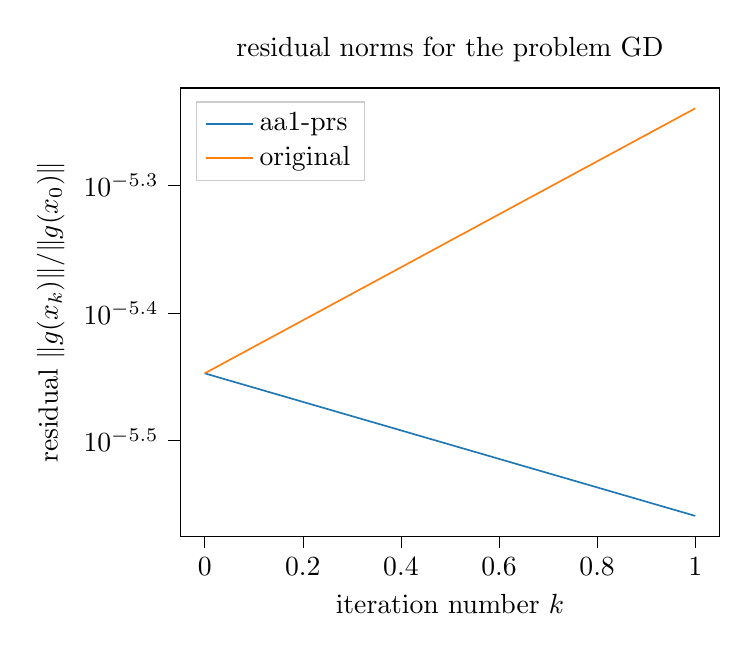
\begin{tikzpicture}

\definecolor{darkgray176}{RGB}{176,176,176}
\definecolor{darkorange25512714}{RGB}{255,127,14}
\definecolor{lightgray204}{RGB}{204,204,204}
\definecolor{steelblue31119180}{RGB}{31,119,180}

\begin{axis}[
legend cell align={left},
legend style={
  fill opacity=0.8,
  draw opacity=1,
  text opacity=1,
  at={(0.03,0.97)},
  anchor=north west,
  draw=lightgray204
},
log basis y={10},
tick align=outside,
tick pos=left,
title={residual norms for the problem GD},
x grid style={darkgray176},
xlabel={iteration number \(\displaystyle k\)},
xmin=-0.05, xmax=1.05,
xtick style={color=black},
y grid style={darkgray176},
ylabel={residual \(\displaystyle \norm{g(x_k)}/\norm{g(x_0)}\)},
ymin=2.65702041966114e-06, ymax=5.97564015934737e-06,
ymode=log,
ytick style={color=black}
]
\addplot [semithick, steelblue31119180]
table {%
0 3.56748104631869e-06
1 2.75673117031559e-06
};
\addlegendentry{aa1-prs}
\addplot [semithick, darkorange25512714]
table {%
0 3.56748104631869e-06
1 5.75950172251125e-06
};
\addlegendentry{original}
\end{axis}

\end{tikzpicture}

		\caption{Residual norms for the logistic regression problem.}
	\end{figure}
\end{frame}

\subsection*{Facility location}

\begin{frame}
	\frametitle{Facility location}
	The aim is to minimise
	\begin{align*}
		F\colon \R^{300}\to\R, \quad y\mapsto \sum_{i=1}^{500}\norm{y-c_i}
	\end{align*}
	for $c_i\in\R^{300}$ with sparsity $0.01$. This can lead to the formulation
	\begin{align*}
		\tilde{f}\colon \R^{500\times 300}\to\R^{500\times 300}, \quad
		z\mapsto \brk*{z_i+2\tikzmark{avg_x_dest}{\avg{x}}-\tikzmark{xi_dest}{x_i}-\avg{z}}_i
	\end{align*}
	with
	\begin{align*}
		\tikzmark{avg_x_source}{\avg{x}} = \frac{1}{500}\sum_ix_i \qquad \tikzmark{xi_source}{x_i} = \tikzmark{prox_dest}{\prox_{\norm{\cdot}}}\brk*{z_i+c_i}-c_i
	\end{align*}
	and
	\begin{align*}
		\tikzmark{prox_source}{\prox_{\norm{\cdot}}}(v) = \brk*{1-\frac{1}{\norm{v}}}_+v\,.
	\end{align*}
	\tikzset{external/export=false}
	\begin{tikzpicture}[remember picture, overlay, node distance = 0.5cm]
		\draw[,->,thick] (avg_x_source) to [in=-125,out=60] (avg_x_dest);
		\draw[,->,thick] (xi_source) to [in=-90,out=60] (xi_dest);
%		\draw[,->,thick] (prox_source) to [in=-90,out=60] (prox_dest);
	\end{tikzpicture}%
\end{frame}


\begin{frame}
	\begin{figure}
		\centering
		% This file was created with tikzplotlib v0.10.1.
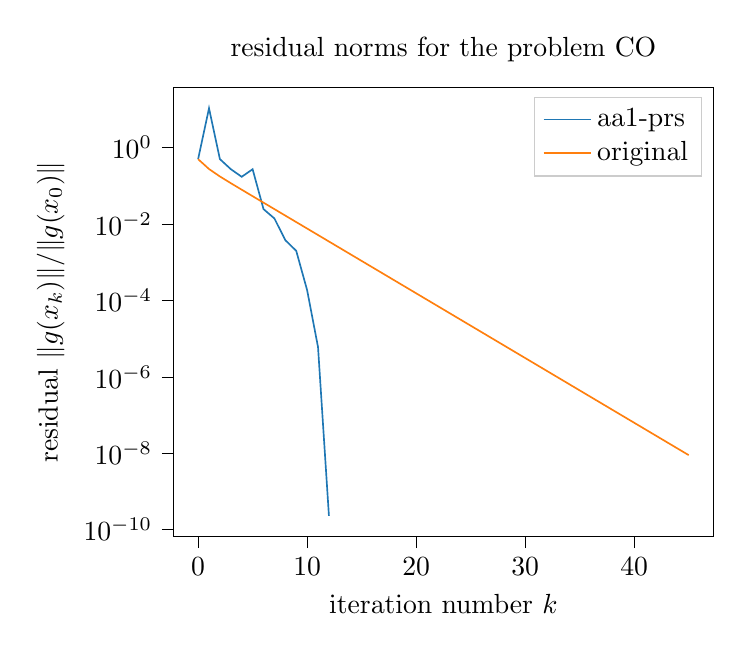
\begin{tikzpicture}

\definecolor{darkgray176}{RGB}{176,176,176}
\definecolor{darkorange25512714}{RGB}{255,127,14}
\definecolor{lightgray204}{RGB}{204,204,204}
\definecolor{steelblue31119180}{RGB}{31,119,180}

\begin{axis}[
legend cell align={left},
legend style={fill opacity=0.8, draw opacity=1, text opacity=1, draw=lightgray204},
log basis y={10},
tick align=outside,
tick pos=left,
title={residual norms for the problem CO},
x grid style={darkgray176},
xlabel={iteration number \(\displaystyle k\)},
xmin=-2.25, xmax=47.25,
xtick style={color=black},
y grid style={darkgray176},
ylabel={residual \(\displaystyle \norm{g(x_k)}/\norm{g(x_0)}\)},
ymin=6.75895940356585e-11, ymax=36.2782620232941,
ymode=log,
ytick style={color=black}
]
\addplot [semithick, steelblue31119180]
table {%
0 0.495588643966115
1 10.6285804099101
2 0.495588643966115
3 0.270976993907102
4 0.171122093577714
5 0.269797398098345
6 0.0244274510783268
7 0.0138820384409515
8 0.00375628732223015
9 0.00197677871866153
10 0.000185167940418084
11 5.98577437452288e-06
12 2.30701834855331e-10
};
\addlegendentry{aa1-prs}
\addplot [semithick, darkorange25512714]
table {%
0 0.495588643966115
1 0.273098074040799
2 0.174466335318158
3 0.11649433193869
4 0.0786362295023986
5 0.0532118801882059
6 0.03602627220658
7 0.0243931681808116
8 0.0165164582075084
9 0.0111830322229492
10 0.00757175864069581
11 0.00512660584009843
12 0.00347104542446171
13 0.00235011304996452
14 0.00159116754254216
15 0.00107731371027646
16 0.000729403537312378
17 0.000493847817458106
18 0.00033436294236866
19 0.000226382552482769
20 0.000153273699758866
21 0.000103774880955939
22 7.02613984375745e-05
23 4.75708921225878e-05
24 3.22081497092301e-05
25 2.1806714540865e-05
26 1.47643621283447e-05
27 9.99629653346881e-06
28 6.76805013547979e-06
29 4.58234728535713e-06
30 3.10250456411087e-06
31 2.10056854640408e-06
32 1.42220200407257e-06
33 9.62910033449992e-07
34 6.5194376579213e-07
35 4.4140227007474e-07
36 2.988539421256e-07
37 2.02340772792762e-07
38 1.36995985545873e-07
39 9.27539189678542e-08
40 6.2799576221216e-08
41 4.2518815038927e-08
42 2.87876035730159e-08
43 1.94908134041768e-08
44 1.31963658200782e-08
45 8.93467750652024e-09
};
\addlegendentry{original}
\end{axis}

\end{tikzpicture}

		\caption{Residual norms for the facility location problem.}
	\end{figure}
\end{frame}

\section{Elastic net regression}

\begin{frame}
	\frametitle{Elastic net regression}
	Our aim is to minimise
	\begin{align*}
		F\colon \R^{1000}\to \R, \quad x\mapsto \frac{1}{2}\norm{Ax-b}^2+\mu\brk*{\frac{1}{4}\norm{x}^2+\frac{1}{2}\norm{x}_1}
	\end{align*}
	with $A\in\R^{500\times 1000}$, $b\in\R^{500}$ and some $\mu\in\R$. From the Iterative Shrinkage-Thresholding Algorithm one obtains
	\begin{align*}
		f\colon\R^{1000}\to\R^{1000}, \quad x\mapsto S_{\alpha\mu/2}\brk*{x-\alpha\brk*{A^\top(Ax-b)+\frac{\mu}{2}x}}
	\end{align*}
	with shrinkage operator
	\begin{align*}
		S_\kappa(x) = \brk*{\sgn(x_i)\brk*{\abs{x_i}-\kappa}_+}_i
	\end{align*}
	and some $\alpha\in\R$.
\end{frame}


\begin{frame}
	\begin{figure}
		\centering
		% This file was created with tikzplotlib v0.10.1.
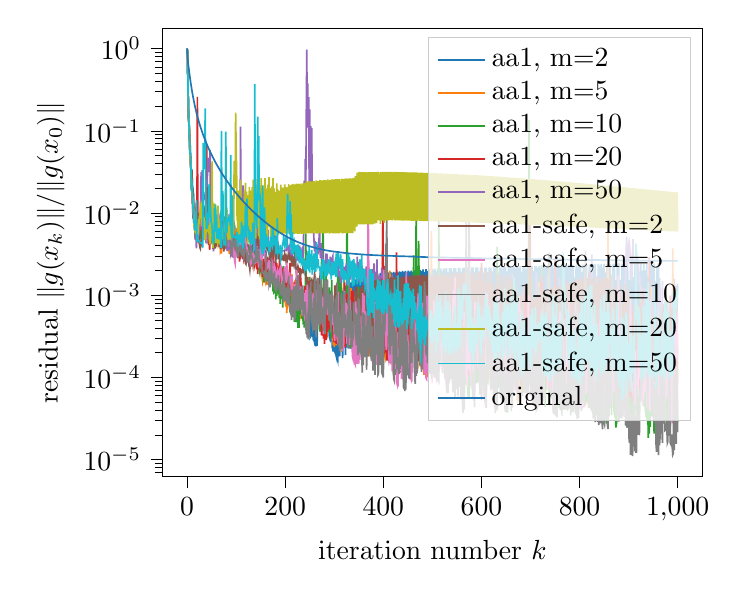
\begin{tikzpicture}

\definecolor{crimson2143940}{RGB}{214,39,40}
\definecolor{darkgray176}{RGB}{176,176,176}
\definecolor{darkorange25512714}{RGB}{255,127,14}
\definecolor{darkturquoise23190207}{RGB}{23,190,207}
\definecolor{forestgreen4416044}{RGB}{44,160,44}
\definecolor{goldenrod18818934}{RGB}{188,189,34}
\definecolor{gray127}{RGB}{127,127,127}
\definecolor{lightgray204}{RGB}{204,204,204}
\definecolor{mediumpurple148103189}{RGB}{148,103,189}
\definecolor{orchid227119194}{RGB}{227,119,194}
\definecolor{sienna1408675}{RGB}{140,86,75}
\definecolor{steelblue31119180}{RGB}{31,119,180}

\begin{axis}[
legend cell align={left},
legend style={fill opacity=0.8, draw opacity=1, text opacity=1, draw=lightgray204},
log basis y={10},
tick align=outside,
tick pos=left,
x grid style={darkgray176},
xlabel={iteration number \(\displaystyle k\)},
xmin=-50, xmax=1050,
xtick style={color=black},
y grid style={darkgray176},
ylabel={residual \(\displaystyle \norm{g(x_k)}/\norm{g(x_0)}\)},
ymin=6.2189496238138e-06, ymax=1.7697757348068,
ymode=log,
ytick style={color=black}
]
\addplot [semithick, steelblue31119180]
table {%
0 1
1 0.876274703014388
2 0.298600999037866
3 0.145348135690287
4 0.136602852316612
5 0.0805920762530411
6 0.0752411835523127
7 0.0503561794195341
8 0.0291941129924188
9 0.0300928169611553
10 0.0311781724526529
11 0.0200523292811158
12 0.0192757782893265
13 0.0171059774502866
14 0.00999711229509404
15 0.0107229032257214
16 0.0116974693145232
17 0.00816306412877159
18 0.00772221800265973
19 0.0069925410502282
20 0.00485392950926771
21 0.00518243657234177
22 0.00522740533155708
23 0.00508754075449725
24 0.00673088789341767
25 0.0085106100019493
26 0.00618877614003522
27 0.00701254866706721
28 0.0081387206388934
29 0.00800574346982429
30 0.00870525089728911
31 0.0105334818176709
32 0.00698736473040824
33 0.0079607879116462
34 0.00828615143938023
35 0.00806935694696941
36 0.00737019218686564
37 0.00509557165027541
38 0.00494560899848085
39 0.0042794776890489
40 0.00635954403822526
41 0.00551923077565319
42 0.00473502801698337
43 0.00557706644176405
44 0.00408839208680265
45 0.00667697987852998
46 0.00575796378032109
47 0.00760263358711143
48 0.0070222318314643
49 0.00785670915414452
50 0.00579479371077961
51 0.00490539690878307
52 0.0105537776878647
53 0.00792936340289781
54 0.00805097232777751
55 0.00982896736087567
56 0.00662541995324538
57 0.0110455718537073
58 0.00903364320391238
59 0.00894332269174603
60 0.00749201795145375
61 0.00626601660253525
62 0.00874260720567795
63 0.00980659534946032
64 0.00924820942670715
65 0.00655944823395743
66 0.00625234099146887
67 0.00648188304481849
68 0.00554451656333562
69 0.00512762479261458
70 0.00560100085341778
71 0.00584408183164445
72 0.00739056994924683
73 0.00805115660105118
74 0.00822506868992428
75 0.00799491102877925
76 0.00910933334774354
77 0.00635377952543695
78 0.00773756893131641
79 0.00611478628643259
80 0.00677660974518796
81 0.00620988614211267
82 0.00473238472707581
83 0.00477286723228329
84 0.00427680530864689
85 0.00660973601445169
86 0.00562259748477694
87 0.0086834064387411
88 0.00543389153533528
89 0.00487383739738421
90 0.0050480740566187
91 0.00632103885841019
92 0.00556461868949226
93 0.00482682563826884
94 0.00555481661294511
95 0.00778521550518858
96 0.00732880775321145
97 0.00688362770362338
98 0.00498891190856403
99 0.00483273894046607
100 0.00555556240075265
101 0.00398203694185856
102 0.00654389656373797
103 0.00586058236860419
104 0.00553996209063832
105 0.00500293866827843
106 0.0039224174574904
107 0.00357178203754569
108 0.00377270565581887
109 0.00371915979043976
110 0.0033085340163252
111 0.00419165515885679
112 0.0044321842196757
113 0.00498197809609319
114 0.00478671473618104
115 0.00515464560540837
116 0.00424844403715698
117 0.00374309807898878
118 0.00370415969986545
119 0.00326644681842047
120 0.00569209618694241
121 0.00427968680558308
122 0.00265764704404021
123 0.00309566867755073
124 0.00266866175592687
125 0.00252385705336605
126 0.00290471269331304
127 0.00307101732146935
128 0.0034628236472327
129 0.00335984129177313
130 0.00340126638119603
131 0.00325747318521626
132 0.00296901808475596
133 0.00328422259972419
134 0.00357327170213648
135 0.00326165591855585
136 0.00337552922454106
137 0.00365403761526415
138 0.00340366171766512
139 0.003628055191527
140 0.00359410321418903
141 0.00326164097314188
142 0.00327603636540935
143 0.00333655130049635
144 0.00297504450046142
145 0.00297431220575661
146 0.00322820917420134
147 0.00290975795301793
148 0.00261459854511514
149 0.00317426940371002
150 0.00300407612069743
151 0.00374976538826653
152 0.00370593184422298
153 0.00330016167405054
154 0.00332238038304637
155 0.00341723937990826
156 0.00309773811876518
157 0.00304655670986148
158 0.00325536135761875
159 0.00293411546823198
160 0.00275320957039173
161 0.00321139813762981
162 0.0028622994036783
163 0.00237050517895342
164 0.00256046722044777
165 0.00244264889382815
166 0.00255232757011808
167 0.00272495180789163
168 0.002608279468887
169 0.0027100480832442
170 0.00306976889425523
171 0.00278136124395291
172 0.00260161028354473
173 0.00272017711180496
174 0.00246448515149491
175 0.00239381749446625
176 0.00244153192374496
177 0.00224723171709371
178 0.00226324468009225
179 0.00242082629344998
180 0.00213372193524825
181 0.00216002105136466
182 0.00214434752530335
183 0.00189975870731536
184 0.00193712035579625
185 0.00171719863270442
186 0.0016913413339104
187 0.00177510239450946
188 0.00160960685608633
189 0.00177203709394052
190 0.00172169197878091
191 0.00175488186316598
192 0.00160461515712864
193 0.00152566083218072
194 0.00161198621902401
195 0.00139366168770533
196 0.00134556146914425
197 0.00134926752717112
198 0.00117774230758777
199 0.00144060237109618
200 0.00128581901609443
201 0.00126586374677554
202 0.00127816395502771
203 0.00134175001068626
204 0.00116460125397761
205 0.00129332543239268
206 0.00131903188810429
207 0.00110156835120643
208 0.00111196239524379
209 0.0011161272364256
210 0.000944160031400512
211 0.00116530173300486
212 0.0012176498690375
213 0.00100884801614628
214 0.000829869994605868
215 0.00117568874788535
216 0.00100879700804633
217 0.000944145392242556
218 0.000890958481006939
219 0.000773425572553311
220 0.000888470544325611
221 0.00105375807576498
222 0.000986708190382638
223 0.00111446034204846
224 0.000922678010594525
225 0.00072786556434706
226 0.000729894421276976
227 0.00082455512015265
228 0.000644522706230811
229 0.000735230919087511
230 0.00086776594811259
231 0.000594693265211378
232 0.000625407762892594
233 0.000801808255065769
234 0.00076689547319389
235 0.000650783480013098
236 0.000879412888556612
237 0.000773053385692481
238 0.00067527586816763
239 0.000751839147660913
240 0.00055712499442272
241 0.000452896518539425
242 0.00038321197976378
243 0.00107521675396875
244 0.000664357127600889
245 0.000493263839942631
246 0.000488091301803344
247 0.00120803079836257
248 0.000386283347192661
249 0.000807956994905144
250 0.000971453671067805
251 0.000307958347413289
252 0.000316192153926059
253 0.000986005049355324
254 0.000314385310841835
255 0.000976436996188001
256 0.000410691765459064
257 0.000293363030003802
258 0.000285052956073466
259 0.000442199737037391
260 0.00025992000678217
261 0.000247556194459953
262 0.000245126625092938
263 0.000932629582324514
264 0.000357012226103561
265 0.000242322428471172
266 0.000475587451211585
267 0.000776637992450989
268 0.00056262387124971
269 0.00077230209680415
270 0.000528467863604187
271 0.000407549224584014
272 0.000361437703428757
273 0.000565117102691557
274 0.000595674132068797
275 0.000547873073321465
276 0.000486167559984953
277 0.000364468858288957
278 0.000325931412760112
279 0.000758953470256293
280 0.000460398078599382
281 0.000602352897807355
282 0.00082823759771171
283 0.000591292909667977
284 0.000929219293448096
285 0.00072586181119255
286 0.000434011890484629
287 0.000407627046495389
288 0.000363695063472756
289 0.00056538628422313
290 0.000312243401776689
291 0.00029772778704103
292 0.000396100681957705
293 0.000318839614080182
294 0.000274602784093825
295 0.000578721103196683
296 0.000230305015737533
297 0.000224007266313771
298 0.000205703752456822
299 0.000519045922493076
300 0.000391843127303301
301 0.000205992265813481
302 0.000198256545112794
303 0.000193765606118013
304 0.000182320947883137
305 0.000544916511611079
306 0.000172023797080489
307 0.000162275400124715
308 0.00167564963943525
309 0.0010384906889946
310 0.000400952391916144
311 0.000180133118107512
312 0.000269707230069985
313 0.00126391193120344
314 0.000235798828851711
315 0.000920615143247019
316 0.00112415306166342
317 0.000171389962841032
318 0.00027025870107379
319 0.00123155464787561
320 0.000232423207778532
321 0.000622400618696794
322 0.00128557414210301
323 0.000188248496885605
324 0.000390174137568516
325 0.00134840850423527
326 0.000229541145575602
327 0.000584844403903162
328 0.00137336065246531
329 0.000224646027258517
330 0.000567848540190064
331 0.00140457637645661
332 0.000225209995174726
333 0.000570518815981079
334 0.00143100215700513
335 0.000222791369326279
336 0.000559963393605158
337 0.00146366249764388
338 0.000220024546462724
339 0.000548071150749682
340 0.00151657697058642
341 0.000216345103723246
342 0.000534256073628689
343 0.00155710937403186
344 0.000215473118821953
345 0.000526870598884988
346 0.00158746150778127
347 0.000216685159745962
348 0.000524639159388505
349 0.00162020358214596
350 0.000216697230796085
351 0.000520095356770237
352 0.00163993322993726
353 0.000216637441297333
354 0.000515956713817094
355 0.00166654545358755
356 0.000211411635823271
357 0.00050826940889506
358 0.00166969632542867
359 0.000218744713899676
360 0.00048951311225487
361 0.00172089872535613
362 0.000212912875921977
363 0.000494739863499323
364 0.00162116881229863
365 0.000249009768818026
366 0.000448772859131775
367 0.00174461979711383
368 0.000217326819649798
369 0.000509008006116486
370 0.00175197914737156
371 0.000217467363572277
372 0.000469756269557775
373 0.00165425607171864
374 0.00025923037350513
375 0.000440509451764863
376 0.00178874472306198
377 0.000223692755407851
378 0.000532385243191729
379 0.00178939750187305
380 0.000219416384749424
381 0.000430893597661579
382 0.0016028043037186
383 0.000270784807191765
384 0.000422762509121024
385 0.00183339897788097
386 0.000228076614962203
387 0.000556671176827414
388 0.0018057785317542
389 0.000215713906218291
390 0.000385882275096262
391 0.00163151096339901
392 0.000264311278893305
393 0.000404798598025166
394 0.00186694627568262
395 0.000231107334487369
396 0.000679806608569336
397 0.00180195759994882
398 0.000217446223705378
399 0.00033089679115647
400 0.00160182092531439
401 0.000256032338979724
402 0.000376762718904466
403 0.00188954664002561
404 0.000233914591553399
405 0.000754272220670714
406 0.00182279991802988
407 0.000216155925936446
408 0.00036247974753269
409 0.00190407328305303
410 0.000233071806750666
411 0.000575468663293062
412 0.00186080210574282
413 0.000221851750770244
414 0.000431456260746182
415 0.00191116493049754
416 0.000234739374943937
417 0.000578030286319609
418 0.0018662940998368
419 0.000222965864872832
420 0.000433904140761864
421 0.00192235683908591
422 0.000235572188230055
423 0.000567681956592502
424 0.00188430680379967
425 0.000225207654302307
426 0.000446857058996945
427 0.0019383644517521
428 0.00023621476359621
429 0.000559831057800436
430 0.00189598717452354
431 0.000226709278294115
432 0.00045539606789637
433 0.00195349971993665
434 0.000236648170193397
435 0.000559766595551062
436 0.00191177352727763
437 0.000227099899435074
438 0.000456241361522967
439 0.00196969686934817
440 0.00023763616224216
441 0.000564692438627508
442 0.00192558483698098
443 0.00022767379329853
444 0.000454530927936515
445 0.00197656744462483
446 0.000239121650032271
447 0.00058929301645295
448 0.00191536413446401
449 0.000227094539597216
450 0.000436259627720609
451 0.00198518204120441
452 0.000240184220806919
453 0.000580630798869503
454 0.0019327571237223
455 0.000229565163171262
456 0.00044786718765257
457 0.00199415434981081
458 0.000242012405179801
459 0.000614788506356843
460 0.00191008503319056
461 0.000228448781909213
462 0.000421275203907404
463 0.00200413212611154
464 0.000243041611678959
465 0.000595260920431909
466 0.00193023793522243
467 0.000231328513663115
468 0.000434437906365273
469 0.00201781103788946
470 0.000245204265309404
471 0.000660229889920061
472 0.00190126427820004
473 0.00022941698908037
474 0.000403418800974596
475 0.00203345248877112
476 0.000245688976127155
477 0.000591237538763436
478 0.0019618415836334
479 0.000235864817561201
480 0.000446936737597806
481 0.00206309564206405
482 0.000247803934000254
483 0.000674978957211969
484 0.00191468679140692
485 0.000233021477592865
486 0.000403964078612395
487 0.00208175600882789
488 0.000249141907030374
489 0.000595683054818413
490 0.00197179664930812
491 0.000238722148733768
492 0.000444150382972061
493 0.00209300337866859
494 0.000249786595613905
495 0.000719227070443317
496 0.00190517891288602
497 0.000233552034791772
498 0.000388216703738786
499 0.00209760938308497
500 0.000252102443892475
501 0.000548649430265323
502 0.00205127176254362
503 0.000249829250846059
504 0.000509235461111106
505 0.00210834156786162
506 0.000248420112574774
507 0.000664179074498694
508 0.00195860844314166
509 0.00023412888559397
510 0.000404354495899358
511 0.00211419841608669
512 0.000257595045639988
513 0.000578519353653649
514 0.00203342532427743
515 0.000247492213015523
516 0.000461506926339139
517 0.00212112330335213
518 0.000249828708116719
519 0.000689454810480768
520 0.00197283275905158
521 0.000234831149472366
522 0.000396842411691915
523 0.00212540672208272
524 0.000260467168071831
525 0.000540169548040532
526 0.00210911297689594
527 0.000261011946933315
528 0.000510752969736052
529 0.00212761249347974
530 0.000262912266718822
531 0.000965266310620254
532 0.00190515295911119
533 0.000242396077459566
534 0.000372182455955698
535 0.00213429501784516
536 0.000263070525642009
537 0.000506452564448219
538 0.00213385200406183
539 0.00026609576440001
540 0.00088185455429291
541 0.00194569845265378
542 0.00024491402247154
543 0.000390116967596152
544 0.00213719011433543
545 0.000264497299077393
546 0.00051029043248524
547 0.00213889301928747
548 0.000268029271625397
549 0.00094650513794177
550 0.00192378029632443
551 0.000248234765005684
552 0.000384692435133042
553 0.00214741293171943
554 0.000264783866129024
555 0.000512118751644402
556 0.00215228092804263
557 0.000267713668882899
558 0.000904159241061944
559 0.00193398921980337
560 0.000248800616241234
561 0.000391325970175805
562 0.00215591588226531
563 0.00026713974620922
564 0.00051111598367538
565 0.00216010988287174
566 0.000270154216288327
567 0.000975423447285879
568 0.00191530007911454
569 0.000250875793555643
570 0.000386110811459082
571 0.00216503567070956
572 0.00026804868466024
573 0.00051052514473311
574 0.00217103554136276
575 0.000269317304261312
576 0.000850448148495845
577 0.00194591578556897
578 0.000251752485634353
579 0.00040092834620477
580 0.00217389455708023
581 0.000269223156399799
582 0.000508958541280942
583 0.00217609604909285
584 0.000271419394579842
585 0.000990781600761954
586 0.00192508307224806
587 0.000254174029272319
588 0.000388874255284182
589 0.00217481665801131
590 0.000267792683542945
591 0.000512820869401317
592 0.00217591922592811
593 0.000269976237244674
594 0.000895118180662194
595 0.00194467320859542
596 0.000253740955040713
597 0.000403842814294871
598 0.00216992735472311
599 0.000269755883999313
600 0.000511492130241025
601 0.00217134928034123
602 0.000273043504587491
603 0.00106850129468
604 0.00187638825534
605 0.000257180480490289
606 0.00038408717001901
607 0.00216479631397689
608 0.000267081401690802
609 0.00051774944954494
610 0.00216173484903994
611 0.000273758066740198
612 0.000978069201109921
613 0.00191355916656929
614 0.000256915594035507
615 0.00039692074873585
616 0.0021674997562479
617 0.000268610022292186
618 0.000520646823423958
619 0.00216485713502785
620 0.000274864825782853
621 0.000885572766726588
622 0.00194581197933853
623 0.00025941225193146
624 0.000414264261579113
625 0.00217245066763423
626 0.000265816254868359
627 0.000555482545154825
628 0.0021560534029631
629 0.000265587196150107
630 0.000516170835202064
631 0.00215412225835306
632 0.000282195361376209
633 0.00117859228689081
634 0.00186454270824664
635 0.000262882425894188
636 0.000391053959876305
637 0.00218387194600915
638 0.000263173247473059
639 0.000533465444589264
640 0.00218473670649573
641 0.000265251161998204
642 0.000659291573620708
643 0.00211393916760469
644 0.000255246369489822
645 0.000455744212601897
646 0.00218827294885481
647 0.000275924584451723
648 0.000518289083338055
649 0.00219805036912894
650 0.000275669749912149
651 0.00101599393711468
652 0.00194487762508736
653 0.000262134001849614
654 0.000399893116680734
655 0.00220625676654214
656 0.000266929147394464
657 0.000534775011658775
658 0.00219509960848738
659 0.000268098324597693
660 0.00065847103239365
661 0.00212636923733669
662 0.000257069140059687
663 0.000456842370658469
664 0.00221668165413201
665 0.000265971182676209
666 0.000536866791519541
667 0.00220230472778996
668 0.00026756193433259
669 0.00066677761442018
670 0.00212602468833933
671 0.000256806963510631
672 0.000450180450463586
673 0.00223635530391549
674 0.000259109791870715
675 0.000557879804384407
676 0.00216340357264919
677 0.000264446700400141
678 0.00049862594987685
679 0.00225571366618639
680 0.000275702704763807
681 0.00120969329102484
682 0.00193726395947969
683 0.000256485798139398
684 0.000380649824830369
685 0.00223813851808558
686 0.000270648656265349
687 0.000508533843495205
688 0.00225967500546113
689 0.000268541864846669
690 0.000833969953912397
691 0.00207603109757905
692 0.000257085610831488
693 0.000417189849289728
694 0.00225484492406873
695 0.000265911416166931
696 0.000542720885055284
697 0.0022209035000773
698 0.000266789612302522
699 0.000534392709441794
700 0.00218145125276304
701 0.000271729257723012
702 0.00049661421573179
703 0.00227045180021502
704 0.000280615620647662
705 0.00120408044293891
706 0.00196059126623678
707 0.000265582469840945
708 0.000392949982394179
709 0.00226253654644369
710 0.000271275335226006
711 0.000532032736523957
712 0.00225073897323587
713 0.000267903033960307
714 0.00066078694139968
715 0.00216463809910272
716 0.000259154418959878
717 0.000443840799392748
718 0.00226100516044679
719 0.000278838514881955
720 0.000528612613619657
721 0.00222523558674912
722 0.000280798687988881
723 0.000777717287664737
724 0.00213107290326532
725 0.000267982089139324
726 0.000424420796564536
727 0.0022965733123541
728 0.000269989091220748
729 0.00078937250954732
730 0.00215680299252101
731 0.000259118701084186
732 0.000419256660019088
733 0.00228992630108564
734 0.00027843824638429
735 0.000520389788871246
736 0.00229699820357527
737 0.000281821558136946
738 0.00112345643870706
739 0.00200423877777832
740 0.000265452603243082
741 0.000386880011013936
742 0.00232628946859767
743 0.000282215578927516
744 0.000521721598515078
745 0.00233743695444333
746 0.000275084970389665
747 0.000763917497743685
748 0.00218314974084624
749 0.000265953468883978
750 0.000430067475799558
751 0.0023479453446068
752 0.000275473722964737
753 0.000598479450263131
754 0.00225023964709575
755 0.000267484059735401
756 0.000478753728963565
757 0.00235388044354847
758 0.00026468148137472
759 0.000712786805750661
760 0.00221845045408723
761 0.000259973314556623
762 0.000418496210123349
763 0.00233739991853605
764 0.00029579060388141
765 0.000502404483497094
766 0.00233966174829283
767 0.000296124200482636
768 0.00138161357450153
769 0.00166819103281712
770 0.000282071996406621
771 0.000360348919315481
772 0.00235209195253439
773 0.000270351015763195
774 0.000615160115258786
775 0.00226784811286276
776 0.00026544053182457
777 0.000470239710472881
778 0.00234853366084839
779 0.000272900912137521
780 0.000822165658645984
781 0.00221957689762805
782 0.000261986715379307
783 0.000407587985669693
784 0.00234801589675146
785 0.000285262452846782
786 0.000506214381838148
787 0.00234234093551609
788 0.000290656085934153
789 0.00140601171676728
790 0.00165027025783192
791 0.000268795593279605
792 0.000345639243239208
793 0.00235603532635262
794 0.0002642143341962
795 0.000790309715576624
796 0.00222457646503887
797 0.000258003093435148
798 0.000420006053826903
799 0.0023598425612619
800 0.000279925975963541
801 0.000529517237735148
802 0.00233530250324562
803 0.000286833087833065
804 0.00107683959481914
805 0.00192574762312723
806 0.00026966816961723
807 0.000378572165967409
808 0.00237674911386653
809 0.0002636678984696
810 0.00054857728709019
811 0.00230894489493723
812 0.000283054289593972
813 0.00050772910794
814 0.00239973343855385
815 0.000287701010412632
816 0.00146775434180289
817 0.00151338054749644
818 0.000263214887804001
819 0.00032819091813391
820 0.00235775014069909
821 0.000263475579335206
822 0.000512318111713169
823 0.00239525732824251
824 0.000262821869219282
825 0.000762647015938439
826 0.00223390477491541
827 0.000255223980607706
828 0.000414562668123307
829 0.0023601256750853
830 0.000286658103931441
831 0.000488049548821831
832 0.00239447467858778
833 0.000288236351948195
834 0.00141649350444048
835 0.00149002316570077
836 0.000274867219301108
837 0.000333300346923501
838 0.00239774538497765
839 0.000261519590068032
840 0.000619678313749737
841 0.00230773348126373
842 0.000258186145609747
843 0.00046753801020658
844 0.00239368141251829
845 0.000280357107308053
846 0.00080618281338172
847 0.00218198159117614
848 0.000269701008598662
849 0.000419115190786637
850 0.00240176735043802
851 0.000265976212079825
852 0.00104972715299054
853 0.00188827022056188
854 0.000259305595024274
855 0.000365301115978075
856 0.00239794317387701
857 0.00026446125067953
858 0.000566149130347784
859 0.00234836862059965
860 0.000262578240836108
861 0.0004893889733943
862 0.00240561043917385
863 0.000266812869037426
864 0.00120292878634961
865 0.00177033328215168
866 0.000256747136587007
867 0.000342155728347561
868 0.00240229261516973
869 0.000274018324235411
870 0.000493943683207656
871 0.0024280636972148
872 0.000280115678313404
873 0.00140591420674587
874 0.00151378823950518
875 0.000258559281798065
876 0.000318971683339338
877 0.00237373668920034
878 0.000277213515312959
879 0.000458837015292594
880 0.00245972333663547
881 0.000280767857094252
882 0.00129404567702803
883 0.00153185078675383
884 0.00025928878733345
885 0.000328071907382073
886 0.00239579583315576
887 0.000258049584273879
888 0.000609060936842064
889 0.0023450998001616
890 0.000255066477772845
891 0.000470344747268719
892 0.00240504715273931
893 0.000280462753543216
894 0.000840367044664703
895 0.00207281021101939
896 0.000277009923242621
897 0.000404558100532754
898 0.00245831741962286
899 0.000282770897814205
900 0.00151895631822889
901 0.00124595809622231
902 0.000263874101495228
903 0.000298028251935109
904 0.002231432260069
905 0.000275013080691537
906 0.000395468197930331
907 0.00243515823703284
908 0.000280767936536645
909 0.00121686802912909
910 0.00166000215176185
911 0.000276478993171142
912 0.000354768722433627
913 0.0024312559779197
914 0.000279361902622848
915 0.00113685305426088
916 0.00168412881019758
917 0.000272462356788626
918 0.000361758138085215
919 0.00242564585967481
920 0.000267134473382826
921 0.000962499396894427
922 0.00191025784989042
923 0.000269205749888654
924 0.000390282823083563
925 0.00242662264415104
926 0.00026368964388213
927 0.000872377591373905
928 0.00198445073183154
929 0.000266491545379361
930 0.000399897410645173
931 0.0024268649090944
932 0.000258926954434286
933 0.000818178973175135
934 0.00200186566805659
935 0.00026703829191563
936 0.000403741219040199
937 0.00242938643401658
938 0.000264110514101563
939 0.00113205027152984
940 0.00167423086068495
941 0.000255443816594517
942 0.000341172543707052
943 0.00237712427552701
944 0.000275314200886655
945 0.000545464457295832
946 0.00236404718517487
947 0.000261862274931928
948 0.000608089610838732
949 0.00227314412590169
950 0.000255100966618417
951 0.000454116136201217
952 0.00242340460003061
953 0.000260871360006488
954 0.00125835011736591
955 0.00147030654121397
956 0.000271473212179439
957 0.000310669587023993
958 0.00227407225361979
959 0.000282293290441137
960 0.000432172768297121
961 0.00245720280894825
962 0.000284107083518066
963 0.00162616030757968
964 0.00103066660067694
965 0.000599924804406667
966 0.00033314228988586
967 0.000219991908351065
968 0.00022318324624698
969 0.000214361424165424
970 0.000551849566312314
971 0.000174832981536125
972 0.000181412889805484
973 0.000655817022081889
974 0.000249943332660361
975 0.00082308189748729
976 0.000336796336477698
977 0.000175125986463712
978 0.000172020167597604
979 0.000878817643603824
980 0.000177471288857194
981 0.000630847168345311
982 0.000506891397973808
983 0.000169013811144921
984 0.000171892922718836
985 0.000350188767112008
986 0.000491933187987055
987 0.00048984618692453
988 0.000715622515267346
989 0.000547620396909226
990 0.000801307539152861
991 0.000772598106243006
992 0.00106486349241296
993 0.00157309831619082
994 0.000994255089432431
995 0.000765813867302777
996 0.000997623958319565
997 0.00130042920214925
998 0.000671683196830722
999 0.000903736032557014
1000 0.00138407931762466
};
\addlegendentry{aa1, m=2}
\addplot [semithick, darkorange25512714]
table {%
0 1
1 0.878313247505329
2 0.302036043755597
3 0.154412321098953
4 0.115797921084635
5 0.0824596905936426
6 0.0488500771616508
7 0.0484004528779488
8 0.0316824300273553
9 0.0187417580571971
10 0.0215778963369487
11 0.0152182896561271
12 0.014135530865804
13 0.0112561803887543
14 0.00789503330070022
15 0.00813275983474266
16 0.00973190920734656
17 0.00492675649002489
18 0.00676692132922726
19 0.00634142938563723
20 0.00571138921406784
21 0.00492994493230125
22 0.00608945192054968
23 0.00710445401616924
24 0.00627889117172222
25 0.00604527071084442
26 0.00737791905039692
27 0.00701177674693237
28 0.00804949649857069
29 0.00642171737035976
30 0.00586561271615954
31 0.00684367339298203
32 0.00551780239915296
33 0.00619415406590104
34 0.00726550604051876
35 0.00788753725901468
36 0.00749971419957758
37 0.011410894233011
38 0.00513471237014873
39 0.0134492640228402
40 0.00510605396841978
41 0.00943739970096822
42 0.00909813550270932
43 0.00845081019133284
44 0.00717618167602234
45 0.00831575042922053
46 0.0066844736794049
47 0.00734665886514956
48 0.0069079887154012
49 0.00477358089964799
50 0.00498508615034437
51 0.0054506875164834
52 0.00569594488765461
53 0.00689134276410634
54 0.00698213343137428
55 0.00778165671538146
56 0.0059074650592673
57 0.00633532115234155
58 0.00502852776007372
59 0.00685666222686877
60 0.00627460970155825
61 0.00491882455220661
62 0.00472532491991581
63 0.00590938935888798
64 0.00610346902087805
65 0.00650454233624549
66 0.0061953017386593
67 0.00564894520091943
68 0.00353877590696365
69 0.00372001050393902
70 0.00321662776446854
71 0.00416025975843884
72 0.00411820733029577
73 0.00580697700287499
74 0.00526369534809992
75 0.00472912367531535
76 0.00532091924102321
77 0.0043115976167269
78 0.00498698724419384
79 0.00598576763013719
80 0.00404419626861379
81 0.00579682009794728
82 0.00500787172077379
83 0.00558772640698686
84 0.00505752919958123
85 0.00398568416572804
86 0.00318715371640916
87 0.00422626035316166
88 0.00546549907278282
89 0.00420772206409335
90 0.00476653882730739
91 0.00496404531202711
92 0.00419105746936218
93 0.00442163464957998
94 0.00646975202193548
95 0.00401934266078674
96 0.00436370977072887
97 0.00554237501393929
98 0.00413297327471534
99 0.00594334851640043
100 0.00468776543705342
101 0.00639900739764182
102 0.00527098936387779
103 0.00463702376419837
104 0.00480183184354608
105 0.00497262409967818
106 0.00567046282052723
107 0.00456032090019473
108 0.00436766173808838
109 0.00405419013715762
110 0.00338763208656503
111 0.00409708411746904
112 0.00401460400040963
113 0.00356171525294573
114 0.0038233573375501
115 0.00434709850465636
116 0.0036583969128792
117 0.00382584962124189
118 0.00374527032153982
119 0.00270258200187315
120 0.00328867856133582
121 0.00358748607739798
122 0.00264880581937112
123 0.00420622803751374
124 0.00315370696285239
125 0.00310825250682775
126 0.00351847269951558
127 0.00361675794157509
128 0.00366734620150197
129 0.00273033485422758
130 0.00348936201618641
131 0.00305609824488366
132 0.00267119798773969
133 0.00314902515778536
134 0.00252469812085348
135 0.00278429693670846
136 0.00253118267188269
137 0.00253285638050817
138 0.00266459977176865
139 0.00266599987559777
140 0.00275526557888278
141 0.0024247360664029
142 0.00255497248434946
143 0.0025687025469419
144 0.00239310857904089
145 0.00251336048073671
146 0.00246271250600474
147 0.00266502696691396
148 0.00229163417547032
149 0.00270030091012262
150 0.00230003709448911
151 0.00200221482225543
152 0.00173815469685866
153 0.00166148589891779
154 0.00147939880955058
155 0.0016169429711096
156 0.00206235532915387
157 0.00158320227910385
158 0.00186223424895945
159 0.00178056211695008
160 0.00155993295157791
161 0.0017546618989001
162 0.00147530295451574
163 0.00136409827496307
164 0.00136798073066162
165 0.00149962315574696
166 0.00175722877522826
167 0.00176542672133443
168 0.00185253118234163
169 0.00200092390407544
170 0.0023407551936183
171 0.00191355268049148
172 0.00235376588241317
173 0.00161101600735974
174 0.0017699861036335
175 0.00179873373889686
176 0.00156349581803983
177 0.00158331462926194
178 0.00148522436406774
179 0.00163333411077088
180 0.00157288939647967
181 0.00159759540453092
182 0.00150557222102845
183 0.00172944565080251
184 0.00121439122115907
185 0.00200545332367195
186 0.00177343174333678
187 0.00150801840898411
188 0.00132486070940338
189 0.00130873565934156
190 0.00112502384588911
191 0.00139652496829489
192 0.00134630965619256
193 0.0011668034615301
194 0.000992847102390742
195 0.000838908306415733
196 0.00110762179240751
197 0.000826957966924548
198 0.000920379318620179
199 0.000882135712158835
200 0.00098008594099982
201 0.000727287251535332
202 0.00161525920567568
203 0.000605357876895991
204 0.000754035387658294
205 0.000875678230450232
206 0.00116848502545013
207 0.000738191960546139
208 0.00188798428339208
209 0.000655083421012153
210 0.000913587654781101
211 0.000723744203191969
212 0.0010327416142643
213 0.000614423486882006
214 0.00179378434217467
215 0.00103075762187281
216 0.000929671207129679
217 0.00144355795581458
218 0.00108664031809663
219 0.000782978581827787
220 0.00151293922384328
221 0.000924108391670959
222 0.000841399003033571
223 0.00070458548535739
224 0.000775460818131528
225 0.000932351972860012
226 0.000585673976213377
227 0.000561858553945347
228 0.000923020261250588
229 0.000487354380728301
230 0.00082673997922777
231 0.000518254521024851
232 0.000803372852279948
233 0.000532547099913514
234 0.00060175711385683
235 0.00112603713574421
236 0.000486362254327547
237 0.000745560136474429
238 0.000945756949159592
239 0.00056739685577535
240 0.000831544759530967
241 0.000491082053749099
242 0.000467467102815677
243 0.000480654792917908
244 0.000848565987299704
245 0.000389102496198903
246 0.00137685520294582
247 0.000498544400623584
248 0.000437702561315563
249 0.000955926999075491
250 0.000692869084909764
251 0.0013384541352822
252 0.0011465842626998
253 0.000723301083582661
254 0.000662072173231182
255 0.000582287368571366
256 0.000617460160899563
257 0.000636085138605437
258 0.000677334238348824
259 0.000535967935277121
260 0.000629603439358863
261 0.000637148213681812
262 0.0005028281322615
263 0.00105196824886831
264 0.00072121920927636
265 0.00049506363066621
266 0.000782204715716231
267 0.000537832928224471
268 0.000493710812656149
269 0.000766944962578813
270 0.00062266017469712
271 0.000820150507282841
272 0.000558548036987686
273 0.000887944260380332
274 0.000651951330449285
275 0.00089816023461565
276 0.000667164890217366
277 0.000534314139652976
278 0.00045110121061245
279 0.000441367989508946
280 0.000375094609321829
281 0.000536730182479558
282 0.000671918358166071
283 0.000360474977511054
284 0.000422399076594589
285 0.000304824014590426
286 0.000455841596941574
287 0.000376391624518184
288 0.000822504689525955
289 0.000505444826572425
290 0.000408340661319951
291 0.000519550730233243
292 0.000540807730964354
293 0.000577664430663689
294 0.000383495922560004
295 0.000308838149079763
296 0.000282238269136335
297 0.000742372004459644
298 0.000246564366706525
299 0.000802961732754627
300 0.000235611324265482
301 0.000301989397931273
302 0.000617490035091881
303 0.00105013329083277
304 0.000245138776089336
305 0.000522999430642333
306 0.00042925656473988
307 0.000344531355436757
308 0.000634001967395675
309 0.000324990192218466
310 0.000475717093303154
311 0.000234060896710296
312 0.000292844557762717
313 0.000242633751291321
314 0.000462000262424937
315 0.000202579385145313
316 0.000597885067450618
317 0.000397296601664847
318 0.000436426258915694
319 0.000548279194363371
320 0.00198378935657405
321 0.0007414966266389
322 0.00043105823557103
323 0.000514612183175668
324 0.000384411978796579
325 0.000266580211498797
326 0.000345928764136556
327 0.000797623547158758
328 0.000272798106240288
329 0.000925862458477649
330 0.000302360660154198
331 0.000334400020425768
332 0.00113093536597521
333 0.000228681840342448
334 0.00121518943239574
335 0.000316296097264662
336 0.000313172174665
337 0.000276542182098966
338 0.000875541134425728
339 0.000253517206336131
340 0.000833516548903238
341 0.000332953236629238
342 0.000395110376812823
343 0.000989938317266141
344 0.000401008692997822
345 0.000742509823998436
346 0.000252014566755075
347 0.000271329429447865
348 0.00023726391362201
349 0.000294516092908102
350 0.000208548627844676
351 0.00109728705265742
352 0.000386194985253309
353 0.00057181054672533
354 0.000615825892875633
355 0.00052788788677208
356 0.000500108230004579
357 0.000298194921783942
358 0.00044067241958123
359 0.000278753629493932
360 0.000488185069042181
361 0.000231559219170025
362 0.000212640289318713
363 0.000736388248512933
364 0.000268279853096326
365 0.000700580280195825
366 0.000302664139390833
367 0.00019529813280301
368 0.000934840858600421
369 0.000202055286252706
370 0.000913746373806845
371 0.00018518023849986
372 0.00021091928411779
373 0.000180950783818799
374 0.00106847061157309
375 0.000283173080102973
376 0.00121591903210049
377 0.000192664193964584
378 0.000204468582475198
379 0.000214841584059921
380 0.000369886086459432
381 0.000426903804134889
382 0.000585359099979476
383 0.000335553407725099
384 0.000731764391862753
385 0.000338988985304625
386 0.00121373637983299
387 0.000282655766381005
388 0.000875907918265681
389 0.000563491953948036
390 0.000693228447674089
391 0.000452192789392173
392 0.000614325964693923
393 0.000526742410389803
394 0.000205462787044489
395 0.000197936860626508
396 0.000181025666307496
397 0.000315863624383687
398 0.000220102206779575
399 0.00676227797970051
400 0.000980813889961559
401 0.000208560209128278
402 0.000193903591283889
403 0.000182315068134351
404 0.000804916947962956
405 0.000160836447888488
406 0.000495171860249756
407 0.000186008205237362
408 0.000193022920239434
409 0.000293619610394925
410 0.000184657723820597
411 0.00126822109080067
412 0.000629998643729107
413 0.00198366989230239
414 0.00166329263991665
415 0.00141624178237286
416 0.000863757099778738
417 0.0013198151230095
418 0.000780723859929748
419 0.000557547795670909
420 0.00114256756550736
421 0.0011692376293366
422 0.000522193581497372
423 0.000671944689072703
424 0.000344167815631819
425 0.000461713018738782
426 0.00102615178112246
427 0.00121610676106398
428 0.000389856658429153
429 0.000350439396362531
430 0.000514978877839115
431 0.000271538443077381
432 0.000557285593510977
433 0.000404257069544215
434 0.00025834216873853
435 0.00133487706560004
436 0.000218433127491826
437 0.000946902647614912
438 0.000614339695538398
439 0.000538296643010104
440 0.000884330707178134
441 0.000338744001054114
442 0.000289443346042375
443 0.000217182512784475
444 0.000192684697387224
445 0.00015256177836921
446 0.000330073898800742
447 0.000128818092030389
448 0.000676993332770716
449 0.000137579066225852
450 0.000136480580825152
451 0.00012150308799499
452 0.000306061225902068
453 0.000382605100833688
454 0.00014464790383675
455 0.000539411599426236
456 0.000359226962396244
457 0.000167250774234245
458 0.000256993293351626
459 0.00116199966000988
460 0.000502412726034337
461 0.0005378443241005
462 0.000404144095942126
463 0.000211491788232198
464 0.000168967070768481
465 0.000145686451840749
466 0.000611393536150212
467 0.000211631090093855
468 0.000184557304795303
469 0.000472179134124751
470 0.000125152861366426
471 0.000272929047577938
472 0.000265499844029521
473 0.000469566557592106
474 0.00039302120646081
475 0.00031288008360135
476 0.000273925058642231
477 0.000138667337730457
478 0.000126772403525387
479 0.000493502588946361
480 0.00031704556535395
481 0.000214060215015453
482 0.000134399260943806
483 0.000107635164206126
484 0.000252100330463466
485 0.000393001643402128
486 0.000367091781652267
487 0.000114938103237971
488 0.000221693341371142
489 0.000101378999363384
490 0.000883045611231673
491 0.000469081369384977
492 0.000420531361846172
493 0.000366865719013043
494 0.000168967742632777
495 0.000517342413357673
496 0.000298724319581205
497 0.000570894810796597
498 0.00601289666524768
499 0.000767102772762342
500 0.00018126192129617
501 0.000155271441540405
502 0.000234667424856193
503 0.000135805618834195
504 0.000140737152619478
505 0.000209576961773845
506 0.000115692284628816
507 0.000538371060229641
508 0.000113833481628032
509 0.000520669548024213
510 0.00059769009557341
511 0.000388548298684674
512 0.000121343744620622
513 0.000120723559506926
514 0.00111114699266961
515 0.000552779147113262
516 0.000578470863822987
517 0.000751946485683745
518 0.000613269580158795
519 0.000303161227203084
520 0.000413159765771758
521 0.00035113870013666
522 0.000648110807253088
523 0.00047075809021635
524 0.000241555835389089
525 0.000672315246346518
526 0.000348645431886624
527 0.000406398329575771
528 0.000243201876292556
529 0.000194982062304743
530 0.000952775102753359
531 0.000246812181810379
532 0.000407478851259754
533 0.000148212804506805
534 0.000142432007633967
535 0.000126040229068076
536 0.000270854208735685
537 0.000161286037633489
538 0.000509895332312469
539 0.000111190609978938
540 0.000129278189184287
541 0.0004302486356377
542 0.000118964045761743
543 0.000643974305009904
544 9.45482347003666e-05
545 0.00101940048410767
546 0.00105955140591252
547 0.000790062052636087
548 0.000253222820211757
549 0.000142445129522866
550 0.000160527345301618
551 0.000530101805666743
552 0.00024037728722975
553 0.000103328278394234
554 9.85265985630318e-05
555 0.000837259152822067
556 0.000142615761918891
557 0.000255167066959562
558 0.000242752620360628
559 0.000321511391393668
560 0.000211247901197844
561 0.000445972144174796
562 0.000147700886189406
563 0.000100251245648149
564 0.000254820001594527
565 0.000183827868722455
566 9.27383415034083e-05
567 0.000740080212029944
568 0.000106077305237782
569 8.49508040644801e-05
570 0.000148272388858809
571 8.53672519944354e-05
572 0.000378024216590429
573 0.000127688297697233
574 0.00106017124685544
575 0.000123512025551765
576 0.000142660414614841
577 9.27407799772341e-05
578 0.00038792858772585
579 0.000474551823549524
580 0.000176267553206945
581 0.000432254721068223
582 0.00038836189593667
583 0.000243518282595231
584 0.000147361375304367
585 0.000126506582538261
586 0.000214951942904186
587 0.000285131626905659
588 0.000312502621701107
589 0.000272693665738581
590 0.00040265900106667
591 0.000198512200948581
592 0.000256720075636851
593 0.000162841896604042
594 0.000609676089740575
595 0.000153490919007701
596 0.000455124261768931
597 0.00011811586689604
598 0.000299807593879701
599 0.000147502602158391
600 0.000180317359794405
601 0.000129239566369274
602 0.000310678369597879
603 0.00041783215862981
604 0.000450781775196876
605 0.000104002400617701
606 9.90759326980031e-05
607 0.000246583046359371
608 0.000121191103622068
609 0.000781615537292218
610 0.000101526900030512
611 0.000571342804702269
612 0.000547043353110943
613 0.000106484420706993
614 0.000101496987542722
615 0.000232466758330404
616 0.000542560064640081
617 9.7312298876756e-05
618 0.00015213318408729
619 7.56406891621294e-05
620 0.000218556567780974
621 8.3665261711809e-05
622 0.000124173316389088
623 0.000142950937189593
624 0.000155084748789466
625 0.000154470819833468
626 0.000537726402857796
627 0.000118085836908428
628 0.000475290546461666
629 0.000170958967732597
630 0.000185885773311403
631 0.000144062080943061
632 0.000107526861426367
633 0.000144163103517527
634 9.73845379646978e-05
635 0.00046782781283711
636 0.000272109066051746
637 0.000225159999786967
638 0.000134568925367155
639 0.000116185768895005
640 0.000617052253319797
641 7.98754127561922e-05
642 0.00016511797166606
643 6.2216600953598e-05
644 0.000145697988903666
645 6.21421786784365e-05
646 0.000168826017961161
647 5.38566253459939e-05
648 5.4119174924735e-05
649 0.000260951389038031
650 0.000306277546914444
651 0.000818239812594527
652 7.96647809588466e-05
653 0.000198184765680255
654 0.000243994843216217
655 0.000172376994551706
656 0.000136504043612617
657 0.000261393550413975
658 7.80722528907346e-05
659 6.71759799116098e-05
660 6.22294717433317e-05
661 6.11967375900528e-05
662 0.000360070022418032
663 7.61084021829234e-05
664 6.80749201397256e-05
665 0.00043006857058758
666 0.000382094661986771
667 0.000142365787581309
668 0.000113975762552576
669 0.000477171289886078
670 9.75108876255422e-05
671 7.5195322266915e-05
672 8.71647336201237e-05
673 5.43897721492802e-05
674 5.21203469370881e-05
675 5.63570853290991e-05
676 6.64740986611609e-05
677 0.000638731448893758
678 0.000986628815673834
679 0.000344824208249491
680 9.51320479833434e-05
681 6.48592340214641e-05
682 0.000490498449136788
683 8.6949810090876e-05
684 0.000146548528820685
685 0.00068023100405753
686 7.85953551310342e-05
687 0.000128999968771427
688 0.000144733627589154
689 0.000122714240843616
690 0.000301333681198768
691 0.000570163799199103
692 0.000107357777854213
693 0.000208917400367942
694 8.59020462737619e-05
695 8.84885246700271e-05
696 0.000121489638761641
697 0.000114424946824629
698 0.000151061079809815
699 8.25717312463922e-05
700 0.000636227644700768
701 9.08381854598203e-05
702 0.000164081770998126
703 0.000113918208902248
704 9.30899876728031e-05
705 0.000663356473432308
706 8.86887553216243e-05
707 9.22447836966187e-05
708 0.000132187234288897
709 0.000138348778323321
710 7.67142326227211e-05
711 0.00025302312616057
712 6.60452186801321e-05
713 0.00055578569889436
714 0.000718049451615888
715 0.000377013845176772
716 0.000821411920952519
717 0.00145551558439237
718 0.00054292697050994
719 0.000172937007570737
720 9.46249248764385e-05
721 0.000247547144271338
722 8.36558044939702e-05
723 0.000127081697704969
724 9.46072341563659e-05
725 7.9129226380902e-05
726 0.00010579650112109
727 0.000203338484702924
728 0.000247082105767193
729 0.000273037149275196
730 6.09568012386111e-05
731 8.13888851919084e-05
732 9.36042403039962e-05
733 8.6086353800916e-05
734 8.13344750103172e-05
735 0.000136233893382938
736 0.000105621891868492
737 0.000967805845722438
738 0.00168572744231102
739 0.000442554258390682
740 0.000865075089169471
741 0.000123738269367587
742 9.27456813844155e-05
743 8.03690276028464e-05
744 0.000727294206643425
745 6.75241201906712e-05
746 5.65962838726651e-05
747 0.000995179586264308
748 0.000106711312452374
749 7.06431393580087e-05
750 7.45686143479004e-05
751 9.69769776252174e-05
752 9.65122063150151e-05
753 0.00106183780142765
754 7.37520186373924e-05
755 7.97296250870215e-05
756 0.000373633890752689
757 6.18445033170486e-05
758 6.20301530108278e-05
759 0.000437632612165331
760 5.42871574515918e-05
761 8.97645370698965e-05
762 5.22408687611825e-05
763 5.14978683645276e-05
764 0.00012838930834763
765 4.49887551300824e-05
766 0.000213665510559461
767 4.19995473260584e-05
768 4.17085262500641e-05
769 0.000106945803388521
770 4.20112997678423e-05
771 0.000400754719413709
772 5.20862378333576e-05
773 0.000258678116055739
774 8.29757639400778e-05
775 7.6290110174719e-05
776 0.000105938653103659
777 0.000291566122536356
778 0.00012327292517292
779 0.000806955316864317
780 0.000319403153175097
781 0.000164866606308439
782 9.324574580842e-05
783 0.000172666005037207
784 0.000438297491711939
785 0.000726399911162846
786 0.000370464930714
787 0.000192170091576408
788 0.000152519056440937
789 0.0001547103166503
790 9.14512837249192e-05
791 0.000236278167101142
792 7.32472081133038e-05
793 6.97948911111669e-05
794 0.000609144415621093
795 8.32538585878276e-05
796 0.000391240781120866
797 0.000115046844921905
798 6.47367503595584e-05
799 5.6948621317314e-05
800 0.000764229585425289
801 8.12395001435665e-05
802 0.000357508895448986
803 5.73230026708994e-05
804 7.12391697192574e-05
805 5.13669429111223e-05
806 0.000129795901627691
807 0.00010025199033126
808 5.75046271877309e-05
809 0.000280624079667371
810 0.000521110081707504
811 7.4910632591662e-05
812 6.89141962894931e-05
813 0.000654486208192199
814 4.94497125574566e-05
815 0.000273133135947725
816 6.41977862078437e-05
817 0.000104021118322349
818 4.25989402656716e-05
819 0.000593169090155541
820 4.67980560960368e-05
821 0.000268930209775007
822 0.000376838297867931
823 0.00024995341286648
824 0.000102533825461636
825 0.000355115944104211
826 9.3736252559197e-05
827 7.26276612055613e-05
828 4.93045572236019e-05
829 4.67561470571498e-05
830 0.000766857103576438
831 8.17146267245043e-05
832 0.000153169171878279
833 4.76417234060461e-05
834 4.88797910436749e-05
835 0.000164470409495226
836 9.5473601779536e-05
837 0.000349008255093616
838 4.9347388773845e-05
839 7.80689335572268e-05
840 0.000168263581676591
841 6.03900870968529e-05
842 0.000450385042153288
843 7.20857587372977e-05
844 8.34295666019307e-05
845 0.000102196286394751
846 4.72206954025996e-05
847 4.2051210464462e-05
848 0.000498968193924226
849 5.25848669654849e-05
850 0.000349085200984413
851 5.00779518745136e-05
852 6.07427436866158e-05
853 0.000121279568772912
854 5.47922723866103e-05
855 0.000391074260103065
856 6.01445819714732e-05
857 0.000274986991996312
858 0.00740033707495247
859 0.000722146147944458
860 0.000498634130954888
861 0.000731480779815828
862 0.000286114445284702
863 0.000174870531046375
864 0.000123431711132273
865 0.000105884128989415
866 9.4664820593476e-05
867 8.43941967796497e-05
868 6.49966993262284e-05
869 6.51133236868261e-05
870 0.00017931591294202
871 0.000684179660462618
872 5.72702350171727e-05
873 0.000209403531125101
874 5.66933524031244e-05
875 8.71128329651398e-05
876 0.000514046022946645
877 0.00058966600710255
878 0.000105000565328413
879 0.000692284516138544
880 0.000342251774972502
881 6.66836305062257e-05
882 7.375037313046e-05
883 0.000734056210193127
884 0.000140417820161373
885 0.000626136153327939
886 7.79464819906306e-05
887 0.000132984353174139
888 0.000347301069631913
889 8.94783364010767e-05
890 7.66664239259904e-05
891 0.000407941290694856
892 7.57119814004521e-05
893 0.000196257607742983
894 0.000419034866231049
895 5.67728769910887e-05
896 5.47236996748833e-05
897 0.000473600266330861
898 5.95294001792641e-05
899 0.000228775984831504
900 0.000125236570600568
901 8.37701039244574e-05
902 0.000364050556446972
903 7.82192987009776e-05
904 0.000377004979871555
905 6.4472523231493e-05
906 6.38580885971532e-05
907 7.08587672681068e-05
908 0.00060894293997636
909 6.08155211188537e-05
910 0.000550839625311253
911 8.9520292829384e-05
912 0.000123598091331267
913 9.3353293108639e-05
914 0.000431470558246361
915 8.3893422687102e-05
916 8.25996024536949e-05
917 5.88704214886237e-05
918 7.12088073741605e-05
919 5.95425437653664e-05
920 0.000724351753660509
921 5.77603568441087e-05
922 0.000251494727111658
923 6.49483875579076e-05
924 7.05759867094187e-05
925 0.000158645163694543
926 0.000117059249316697
927 0.000569334681946022
928 6.05501703864325e-05
929 0.000582433368546143
930 0.000621651057329224
931 7.42435600722695e-05
932 7.09358725221085e-05
933 0.000648809173750491
934 6.05567850073262e-05
935 0.000499784467373708
936 0.00029528867861043
937 8.25406942884851e-05
938 7.40106301942061e-05
939 0.000579264765228196
940 6.45758319408977e-05
941 0.000288848027441096
942 0.000782659856652693
943 7.89596450086389e-05
944 5.27908969593012e-05
945 5.16952068594873e-05
946 0.00124150617795066
947 0.000122338053501984
948 4.89766970844872e-05
949 4.17106653198359e-05
950 0.000539876003666819
951 4.91351223505171e-05
952 0.000419854738822977
953 5.04970459714366e-05
954 8.35983630780046e-05
955 3.94360263490099e-05
956 0.000161687188333413
957 4.5778624881626e-05
958 0.000331993735366562
959 0.000189965919632393
960 0.000137456279399939
961 4.03560991636861e-05
962 3.84271807519812e-05
963 0.000639903151436003
964 4.45982918892986e-05
965 0.000377634197744067
966 0.000261222242947032
967 7.84075966608582e-05
968 4.40784385166256e-05
969 4.27791623512725e-05
970 0.000651727154126267
971 4.52378700117384e-05
972 0.000179058135393534
973 4.47699159611941e-05
974 0.000859421874318425
975 4.17588514162996e-05
976 0.000399534591044711
977 0.000354734283537116
978 0.00044381408892439
979 5.81261053441527e-05
980 5.53268959441438e-05
981 0.000317706793397109
982 4.37360441855836e-05
983 0.000348001931939448
984 4.67901081702302e-05
985 4.66649595207993e-05
986 0.000712646670327286
987 7.03467859866468e-05
988 0.000354155933562467
989 0.000363703250487753
990 0.00371774237969395
991 0.000429376996007269
992 8.04843913597452e-05
993 5.53062626343222e-05
994 7.18940320276791e-05
995 0.000127054333750816
996 4.2483473611942e-05
997 3.23654955626113e-05
998 0.000106485772863367
999 2.83202983924014e-05
1000 0.000337160175282865
};
\addlegendentry{aa1, m=5}
\addplot [semithick, forestgreen4416044]
table {%
0 1
1 0.875490423449638
2 0.318520827582027
3 0.150027874064201
4 0.128307269392597
5 0.0798505015207293
6 0.0497987965335321
7 0.0476203160397432
8 0.0347242432515865
9 0.0203068267133236
10 0.022904422439839
11 0.0150327576813464
12 0.0153953114205704
13 0.0106102274301572
14 0.00963334398479963
15 0.00807556671639034
16 0.00595244956066956
17 0.00708106622461955
18 0.00567626203343227
19 0.0073084104725024
20 0.0058378286709687
21 0.00961294982846169
22 0.00894434718144819
23 0.00697734764312482
24 0.00553405300968376
25 0.00635712272663954
26 0.00457224609390407
27 0.0064274415169276
28 0.00533201825155749
29 0.00821472216669448
30 0.00507216241920556
31 0.0106228304520742
32 0.00678893319219033
33 0.0068495003559414
34 0.0123806008495896
35 0.00838307556859348
36 0.0114429026347379
37 0.0115227989381375
38 0.00967972501732582
39 0.0102568379539917
40 0.00807851269759357
41 0.00784552044144417
42 0.00642031288524475
43 0.00782553828833132
44 0.00708803291844289
45 0.00633076702363263
46 0.00491631870033647
47 0.00534199777632487
48 0.00637285242904421
49 0.00701959712344287
50 0.00726388098506148
51 0.00755460255533806
52 0.00527966824952424
53 0.00760733841457578
54 0.00450945878724656
55 0.00486291269141415
56 0.00453889105658463
57 0.00726242672392227
58 0.00610525873024649
59 0.00939928280378972
60 0.00802896762670056
61 0.00513424835100172
62 0.00854081767806312
63 0.00524092630380924
64 0.00776873405489454
65 0.00762506446299544
66 0.00696577283499717
67 0.00788120407848611
68 0.00702875589825981
69 0.00641388325880993
70 0.00688232606039798
71 0.00456001304023542
72 0.00676179161438231
73 0.00498552822521284
74 0.0074595594918258
75 0.00586671343505703
76 0.00835599285037319
77 0.00842852173677902
78 0.00768929016877255
79 0.0054644699511795
80 0.00488176221062563
81 0.00608352621152081
82 0.00565212794795335
83 0.00667255935696223
84 0.00681655203070928
85 0.0081474519749407
86 0.00677209578422414
87 0.00759063303940208
88 0.00748644396003776
89 0.00667472961271252
90 0.00430157961737624
91 0.00406212357241589
92 0.00350801382575747
93 0.00415252765692968
94 0.00423374815158317
95 0.00346634536878785
96 0.00401468041883756
97 0.00340159034940921
98 0.00387199682647439
99 0.0038213098819417
100 0.00408458259333781
101 0.00356753532951582
102 0.00291759860774873
103 0.00343385238832412
104 0.00280167654168336
105 0.00353797324961782
106 0.00331234799731876
107 0.00368591984441962
108 0.00417460241875026
109 0.00375765873503134
110 0.00375320312955861
111 0.00446009214085766
112 0.00409605442942491
113 0.00436485329770005
114 0.00407589703338269
115 0.00489511883887964
116 0.00372481088973653
117 0.0043466990203901
118 0.00401549807523283
119 0.00338336941660044
120 0.00478594267486659
121 0.00424515071352622
122 0.00377644337200387
123 0.00328629942642349
124 0.00361294091239153
125 0.00312464788814883
126 0.00399042199293646
127 0.00352863381488697
128 0.00374461107172401
129 0.00346071364918651
130 0.00321645559286506
131 0.00329649230811475
132 0.00319623823565733
133 0.00315690961007037
134 0.00297865526689045
135 0.00275983127622436
136 0.00308530540418788
137 0.0025111312179194
138 0.00381593681273101
139 0.00264289044079478
140 0.00326883200412333
141 0.00280801986612502
142 0.0028617407789272
143 0.00283622786901271
144 0.00264432691519037
145 0.00237014513421721
146 0.00211609319159591
147 0.00207070528673326
148 0.00192219666278177
149 0.00246189206033778
150 0.0023223511427477
151 0.00284942061761816
152 0.00184636323138985
153 0.00272202612626416
154 0.00220822316856083
155 0.00179584773116769
156 0.00172801526072423
157 0.00142356686261373
158 0.002378862634954
159 0.00241399223853759
160 0.00186867569082529
161 0.0017700428954358
162 0.00203410169317773
163 0.00147960861590206
164 0.00262219456812007
165 0.00239460860613298
166 0.00198534597172549
167 0.00175214813705762
168 0.00148107542729977
169 0.00143008879623105
170 0.00180559215341731
171 0.00157029603032101
172 0.00149707145494259
173 0.00142553890559236
174 0.00155344050957303
175 0.00119056796290364
176 0.00121797615628915
177 0.00108370792663375
178 0.00111353953203212
179 0.00112113679064697
180 0.00154168817368294
181 0.000892794097897929
182 0.00210106307914118
183 0.000983971500817059
184 0.00155542173624394
185 0.00122445134146543
186 0.00162207055061283
187 0.00113213149939381
188 0.000923965531061227
189 0.00115790182374228
190 0.000782688317714329
191 0.00155770566226274
192 0.00135924101855328
193 0.000900817983447769
194 0.00208914394804423
195 0.00070437018585749
196 0.00224886891612532
197 0.00128729309692367
198 0.00125861297273663
199 0.00123072780584917
200 0.00104521463635949
201 0.00103970349879267
202 0.000913836586276976
203 0.00144644423405692
204 0.000943440089198715
205 0.001054612819369
206 0.000835063584582278
207 0.00147730627054841
208 0.000760492206606243
209 0.000956746797749645
210 0.000614280427171504
211 0.000819566819470992
212 0.000688745326690475
213 0.00122911898919778
214 0.00060373946569793
215 0.000660435431606739
216 0.000712846075204861
217 0.000755814947729199
218 0.00113444509799703
219 0.000473332890328641
220 0.00105445547429111
221 0.000588326678460831
222 0.000469502945503194
223 0.000698546235937716
224 0.000642407012209075
225 0.000677836381526355
226 0.000400916527786186
227 0.00142182487915042
228 0.000399874593040024
229 0.0010418506974273
230 0.000647871445469121
231 0.000641385293802619
232 0.000586604254683639
233 0.00124635196227379
234 0.000536823010073509
235 0.000543509268794405
236 0.000534977316811429
237 0.000440575355292823
238 0.000853507972992611
239 0.000404273038989045
240 0.000967059320758545
241 0.000414744267263501
242 0.0056624280644116
243 0.000888083717904969
244 0.000428815228475293
245 0.000442352667985684
246 0.000850847985880848
247 0.000534928919163834
248 0.00143445356902436
249 0.000434951850207478
250 0.00167333133999264
251 0.000609536258359041
252 0.00100168025551831
253 0.000835348976520303
254 0.000769551209298388
255 0.000875553622453145
256 0.000603790292170189
257 0.00149596985018855
258 0.000496915657237222
259 0.000736201571932602
260 0.000703166627196521
261 0.000724295056644842
262 0.000646080496599134
263 0.00119690018005503
264 0.000878443603514234
265 0.000457074559271666
266 0.00062223085030936
267 0.000492637677609636
268 0.00114613677695508
269 0.000492669119928731
270 0.00138742968688892
271 0.000359480560087165
272 0.000885603762587908
273 0.000640535384713645
274 0.0024248205787314
275 0.00291404033551086
276 0.00170945886289432
277 0.0103543035947631
278 0.00202072086150097
279 0.00112941679627852
280 0.000636645675947396
281 0.000737527850147042
282 0.00101187866764804
283 0.0023273102966012
284 0.000930959214531454
285 0.000420856931254829
286 0.000714635310899247
287 0.000376590236251758
288 0.000646248743652799
289 0.000354011156717926
290 0.0012475755403088
291 0.000487869717226823
292 0.000467748166002811
293 0.00113580908025232
294 0.000299933490794679
295 0.00152314873658308
296 0.000342656009339992
297 0.000364662713357632
298 0.000451147990134982
299 0.000417843263028646
300 0.00072986237163427
301 0.000685431687913963
302 0.000843400388534971
303 0.000551957372918111
304 0.000707697661186859
305 0.000915920167365319
306 0.000467286783401798
307 0.00199214338449988
308 0.00245727524294454
309 0.00159642237887924
310 0.00172787651347268
311 0.00100378299591361
312 0.000619708869390426
313 0.00072757912126557
314 0.00150431627568679
315 0.000546959774018152
316 0.000601409120145226
317 0.000469226916621971
318 0.000543007434303477
319 0.000656158245389666
320 0.000283893743350901
321 0.000249434038039036
322 0.000394638137438846
323 0.000239557010062923
324 0.00104894273171129
325 0.000604776831787237
326 0.0181069636035034
327 0.00117849136342666
328 0.00278956690762174
329 0.000708384843836683
330 0.000514161565937494
331 0.000329021223707627
332 0.00027828235967422
333 0.000403543111337244
334 0.000225731538339156
335 0.000665591351837642
336 0.000256655224805979
337 0.000285343315640817
338 0.000653126750412679
339 0.000301635550624169
340 0.000787397945546908
341 0.000318518213312313
342 0.000294064097045782
343 0.0008364080925361
344 0.000198700355991909
345 0.000587590250895293
346 0.00039048598779342
347 0.000862815124932137
348 0.00051581078220383
349 0.00127191238648257
350 0.000234064266654742
351 0.00120164601444495
352 0.000447558152077626
353 0.000405886632925132
354 0.000291877618659088
355 0.00030256444313263
356 0.000776854902480781
357 0.000319125865909126
358 0.000903246421384634
359 0.000227500509130496
360 0.000978312517195334
361 0.000215990941951313
362 0.000769671284562199
363 0.000720784030502265
364 0.000400620895354971
365 0.000364394366720348
366 0.00137945261127096
367 0.000279350020977356
368 0.000302581330208528
369 0.000429944688169504
370 0.00137242451346962
371 0.000313128588785656
372 0.000663307334422546
373 0.000247021079533688
374 0.000487554219800812
375 0.000223696402543174
376 0.000728517662763835
377 0.000209515945949658
378 0.000485897492339441
379 0.00023137091755942
380 0.000606144533601441
381 0.000170738220616397
382 0.000449767764139231
383 0.000190225452889677
384 0.000495530792579152
385 0.000245859384562082
386 0.000203712756932294
387 0.000169422521713965
388 0.000516468716715572
389 0.000214806461072825
390 0.0010678477334768
391 0.000148919473353842
392 0.00094262494633332
393 0.000244335512135286
394 0.00044108830366659
395 0.00029425209605045
396 0.000355317608983754
397 0.000233354611871641
398 0.000362305778082957
399 0.000268389993091486
400 0.000147346287701175
401 0.000822170830916363
402 0.00019878052921904
403 0.00069503906016549
404 0.000296121253665141
405 0.00184312523168043
406 0.000540935419414838
407 0.000570352805565291
408 0.000401752792181608
409 0.000247641561268168
410 0.00021222229437195
411 0.000329889826451655
412 0.000272009773408639
413 0.000219804327839173
414 0.000150191330528609
415 0.000285211837476353
416 0.000200002979458566
417 0.000566522362696863
418 0.000832498691343113
419 0.000351550096959202
420 0.000141318477552869
421 0.000110788707347927
422 0.000252133291803478
423 0.000355823349927702
424 0.00010756836882253
425 0.000483808783522188
426 0.000231738405006418
427 0.000682982457278933
428 0.00017300476858592
429 0.000178670265330796
430 0.000137716443113161
431 0.000138617384882916
432 0.000290763569680978
433 0.000252643777199424
434 0.000535711711718158
435 0.000114468470046394
436 0.000388423924474793
437 0.000145302146454226
438 0.000727531411384458
439 0.000838422967653171
440 0.000550974381086534
441 0.000346126494168737
442 0.0003227572920909
443 0.00102273551243105
444 0.000260826279412817
445 0.000161385346039331
446 0.000418486905164105
447 0.00108222863886074
448 0.000125268888329687
449 0.00114316446893267
450 0.00050100011641744
451 0.000194835705184856
452 0.000186875994321856
453 0.00102401417806032
454 0.00015852892895421
455 0.000724399025968748
456 0.000278264535934286
457 0.000409842572475779
458 0.00018075434568279
459 0.00102237297943428
460 0.000587117600009455
461 0.00100223901586777
462 0.00305430814041467
463 0.000666280957685856
464 0.000326242666966063
465 0.000156559279759901
466 0.000834354103199555
467 0.0118397789837717
468 0.000412569167380942
469 0.000227603137401606
470 0.00067015784735428
471 0.000574270957463696
472 0.00457022167705999
473 0.00141065780555959
474 0.000958042519801484
475 0.000751037301461992
476 0.00153157625503811
477 0.00118310397198322
478 0.000494796979564662
479 0.000335872455443411
480 0.000431232799711658
481 0.000341282679795324
482 0.000273013256401567
483 0.000287859678547181
484 0.000193962616642505
485 0.000171902842018528
486 0.000190079281706121
487 0.000124524021539354
488 0.000306570823931831
489 0.000203958095974109
490 0.000942168904570099
491 0.000127530788494586
492 0.000409256986634434
493 0.000125320861159496
494 0.000329223239003454
495 0.000215843904445458
496 0.000151566637545476
497 0.000136633435878775
498 0.00113443363466152
499 0.000115516540275336
500 0.000421022217605247
501 0.000134197252821488
502 0.00134922170113566
503 0.000117689084054943
504 0.000341399215957914
505 0.000306254582690818
506 0.000394821413028144
507 0.000184919074162613
508 0.000118713136650916
509 9.56835044921771e-05
510 0.000150438425703547
511 0.00112786285082277
512 0.00010641052543019
513 0.00843094293841755
514 0.00123219575635103
515 0.000428340599042983
516 0.000166309777489088
517 0.000721919432703724
518 0.00015762653370872
519 0.0011044837003078
520 0.000172525156853403
521 0.000113300291178764
522 0.000458261660084132
523 0.000429508735169828
524 0.000132738200967427
525 0.00157323490411624
526 0.000133758285026114
527 0.000393145583301025
528 0.000161931053569993
529 0.000144782482468892
530 0.000127979664845328
531 0.000429760751048725
532 0.000143341329584495
533 0.000610067497258209
534 0.000114543645073718
535 0.000696974221673627
536 0.000151855565208266
537 0.000334010230918821
538 0.000121538759037298
539 0.000122339439224053
540 0.000143252441011341
541 0.000112183399687881
542 0.000710616262710815
543 0.00011164495279933
544 0.000529165836574425
545 0.000124298518827927
546 0.000715700394490343
547 0.000326902319732162
548 0.00109560568889536
549 0.000869530612404979
550 0.00105679124778263
551 0.000658128406757535
552 0.000579265003881019
553 0.000304015031635868
554 0.000192042330202041
555 0.000197356090001178
556 0.000539940823791345
557 0.000154255830519909
558 0.000494749101470152
559 0.000141879198111862
560 0.000276764984883207
561 0.00025375790957826
562 0.000107109505689575
563 9.54910786924341e-05
564 0.000437272495200886
565 0.000180087147538565
566 0.000922471891844133
567 9.70358950264121e-05
568 0.00012240205118554
569 8.06055339847177e-05
570 0.000115762861084159
571 0.000293175529944567
572 7.94817968402073e-05
573 5.80895290262262e-05
574 0.000596120921423968
575 5.8618459210192e-05
576 0.000701593817268483
577 7.82294617497748e-05
578 0.0017248959174166
579 0.00155916497337721
580 0.000268867760646375
581 0.00013764684013173
582 0.000247466411177019
583 0.000425396762225499
584 0.000109099070459253
585 0.000102790887955035
586 0.000733515973307358
587 0.000153398422920509
588 0.000286606162154545
589 8.51439545470167e-05
590 9.29468483212982e-05
591 8.56798852131272e-05
592 0.000178743833079428
593 0.000113451209137163
594 9.54643508417314e-05
595 9.1870609362738e-05
596 0.000374516592535969
597 6.23361350193172e-05
598 0.000316217037848697
599 8.24620736335327e-05
600 8.28802943377665e-05
601 0.00019415331540513
602 8.85098575611466e-05
603 0.000364541991121229
604 0.000299094654081785
605 0.000653625911210385
606 0.000501778553049134
607 0.00030125474460978
608 0.000411835842898212
609 0.000122005273149929
610 9.25272098994942e-05
611 0.000619063209232724
612 0.000407970557268269
613 8.16612970402117e-05
614 0.00100229953764058
615 0.000253695947932329
616 0.000344247278778074
617 0.000779781322484892
618 0.00026646509792433
619 0.00139020631877309
620 0.000193705234435159
621 0.000127332199251423
622 8.03415878392568e-05
623 0.000247783193459122
624 0.000194102505309918
625 7.78154453633768e-05
626 0.000643563548064829
627 0.000688646211847333
628 0.000778336279014247
629 0.000438388033635712
630 7.53885881449287e-05
631 7.52955246205874e-05
632 0.00390646920518654
633 0.000669492723722584
634 0.000175846090558617
635 7.40487444949847e-05
636 0.000125154335944185
637 8.86985345553181e-05
638 0.000366769255365761
639 8.01205393625849e-05
640 0.000237203984815706
641 0.000637186328866221
642 0.00119246408470677
643 0.000296653013309543
644 0.000642649141083518
645 7.1322960023218e-05
646 0.000307476114992783
647 9.93727867972396e-05
648 0.000752225609223963
649 0.000127465025131887
650 3.97377302795007e-05
651 3.91053167360658e-05
652 0.000372231604058992
653 3.72229497967153e-05
654 0.000261626643218694
655 6.74228287810046e-05
656 7.30107255768968e-05
657 0.000515482483298244
658 7.5484731591191e-05
659 0.00012028945549878
660 0.000114204712275461
661 0.000122209286221598
662 9.62447952540452e-05
663 0.000508835599923123
664 0.000115497986542538
665 7.68733676680723e-05
666 0.000248034531337671
667 0.000844712834875198
668 0.000197092436051167
669 0.000286316489930094
670 0.00128725332493979
671 0.000780109907281469
672 0.000343693436266193
673 0.000517051016687365
674 0.00029637063626533
675 0.000762783337528524
676 0.000148131622911084
677 0.000129212203664016
678 0.000562508001663955
679 0.0009158419899177
680 0.000334984704592783
681 0.000338619074442825
682 0.00076089114995926
683 0.000116934161731064
684 0.000110833678535606
685 0.000299768201949801
686 8.61494047687196e-05
687 0.00032066052484927
688 8.17969768638138e-05
689 0.000122262148238795
690 8.22838681034848e-05
691 9.33452763802281e-05
692 8.88872978695597e-05
693 8.40725945675784e-05
694 0.000636176799229639
695 0.000289449511037626
696 0.0010192112785463
697 0.134954471577793
698 0.00078909519478394
699 0.000426422712935654
700 0.000589687324410203
701 0.000154752523168129
702 0.00161991940794508
703 0.000108951095133119
704 0.000180769444231004
705 0.000260228516584909
706 0.000110903957890892
707 0.00011541756000036
708 0.000220125210219875
709 8.59510931605308e-05
710 0.000101515469003593
711 7.95252216665238e-05
712 8.30602978413533e-05
713 0.000264871433276544
714 0.000374945492701329
715 0.000417515911506318
716 0.000107134769334458
717 0.000127835506342827
718 0.00125308660777597
719 8.42817641577105e-05
720 7.47049780891395e-05
721 0.000762926533364878
722 0.000266663826508432
723 0.00232666423994338
724 0.000270330261779067
725 0.000111128201604731
726 0.000100204610258179
727 6.03255977749488e-05
728 6.40169230040684e-05
729 0.00035551644856097
730 4.33764554977058e-05
731 0.000176422742827881
732 7.06147651016346e-05
733 0.000221441018286267
734 0.000257508819381358
735 0.000126059792310413
736 0.000190918392083292
737 0.000139915337361955
738 6.52595330019053e-05
739 0.000133365425928767
740 0.000143463328461664
741 0.00014856798638312
742 5.8299982478017e-05
743 0.000161218475445392
744 7.64946726166408e-05
745 0.000161817273626203
746 0.000625902183877608
747 8.04823089449316e-05
748 9.18720473302099e-05
749 4.95965943436147e-05
750 4.57795272106995e-05
751 0.000393436225246921
752 8.07343171696198e-05
753 0.000316185841461918
754 7.74881427738933e-05
755 8.51970431671043e-05
756 8.84399104088713e-05
757 0.000884433553169001
758 4.99098917116292e-05
759 4.2283203840798e-05
760 0.000127124514381374
761 3.98284259808541e-05
762 0.000598991742452556
763 4.76336814876404e-05
764 0.000402531248032591
765 0.000101764214197851
766 4.94991314528779e-05
767 8.25477857000492e-05
768 4.07607073406858e-05
769 0.000327842248931396
770 0.000884166443656482
771 9.60730686544789e-05
772 6.93398655116494e-05
773 0.0002908853813473
774 4.28137099705001e-05
775 4.17809121983032e-05
776 0.000316759989991139
777 5.63200886845943e-05
778 0.00105915567249166
779 4.48149087693528e-05
780 6.8508287453184e-05
781 5.03524181150442e-05
782 4.90790156885197e-05
783 0.000529568903130168
784 9.80318431238445e-05
785 0.000257544092782334
786 3.98325413172008e-05
787 9.6370908584375e-05
788 4.20082078704922e-05
789 0.000171671245875809
790 4.13731569901805e-05
791 0.000124924175821998
792 0.000356907220896308
793 6.1982321003677e-05
794 4.95412601535001e-05
795 5.76005411375027e-05
796 3.55261893671856e-05
797 0.00013201197723863
798 5.33221632293092e-05
799 0.000287323323949689
800 4.51350024663721e-05
801 0.000154770548493834
802 0.000136985256259759
803 0.000707533382154619
804 6.52502687877493e-05
805 5.18438277481539e-05
806 0.000285694301609658
807 0.000129714858347387
808 0.000812339734582
809 0.000353154287064119
810 4.51428921207334e-05
811 0.000213479992467842
812 4.63098382490214e-05
813 5.54194974183979e-05
814 6.42906493377346e-05
815 5.14910580179e-05
816 0.000281818487050197
817 7.13434389107993e-05
818 0.000108320967408769
819 4.55005771212963e-05
820 0.000101569434045386
821 4.76588664514748e-05
822 0.000436997602333458
823 4.73219287260364e-05
824 8.1047366078032e-05
825 0.000123834481537097
826 3.9351416301896e-05
827 3.6387793975673e-05
828 0.000291304686313439
829 4.39941009728779e-05
830 3.16302492793278e-05
831 5.43233084896588e-05
832 3.1907125592867e-05
833 0.000249817575027591
834 3.52584926849875e-05
835 0.000282904007103096
836 0.000147324735214367
837 4.38761993480011e-05
838 4.48637572507758e-05
839 0.00033362259636928
840 3.47019115277467e-05
841 3.57186611022112e-05
842 7.40946407315854e-05
843 0.000279681064566635
844 2.90527673569832e-05
845 0.000670125506851722
846 0.000606585924667777
847 0.000769215340462192
848 0.000253212286705605
849 6.42608557937602e-05
850 5.35170242597712e-05
851 5.59523037200888e-05
852 5.01923779371662e-05
853 3.22605910993969e-05
854 7.52641586440475e-05
855 2.74395299591656e-05
856 0.000142264232653435
857 5.09696727607249e-05
858 5.15678718203464e-05
859 4.95599277120316e-05
860 0.000217647423138159
861 5.43621072886638e-05
862 9.01644722495362e-05
863 4.27733693500131e-05
864 0.000247807217545997
865 3.47762513547918e-05
866 5.3325631045369e-05
867 5.23420657380459e-05
868 6.54759914559339e-05
869 0.000450236519118186
870 3.98973191401472e-05
871 3.68524958037815e-05
872 3.24438665257887e-05
873 0.000192674357259245
874 2.4530850262642e-05
875 2.66971828513209e-05
876 2.95139258008492e-05
877 0.000124750793529312
878 3.52361042983965e-05
879 5.27593535091301e-05
880 5.18281750541053e-05
881 4.71893367257673e-05
882 0.000107794334757417
883 3.21590476814338e-05
884 0.000504849066793856
885 4.96649194233123e-05
886 0.000294326638066594
887 0.000306580583139965
888 0.000504907359328197
889 3.47399005563986e-05
890 0.000123286231910972
891 3.56632554028323e-05
892 3.30033260380829e-05
893 0.00035484965127443
894 2.59108482697993e-05
895 9.11697668953186e-05
896 2.58454794747482e-05
897 9.86859102258494e-05
898 2.61228945449345e-05
899 0.000113606498328233
900 5.50592951217098e-05
901 0.000200660126752824
902 0.000326361097361512
903 3.62411244091064e-05
904 3.45911744061721e-05
905 0.000203009898054238
906 2.77991162175441e-05
907 5.37773386235942e-05
908 3.26588864738249e-05
909 0.000162892028828718
910 2.69397355863245e-05
911 0.000221409991993934
912 0.000372129573077934
913 0.000280700596058666
914 5.07940267758151e-05
915 4.65652859776978e-05
916 2.63564161200171e-05
917 2.20606252632807e-05
918 0.000134762758105875
919 2.07814916839866e-05
920 0.000131302890959511
921 2.33229980364474e-05
922 0.000118220366991195
923 0.000475709160244031
924 0.00149037864180567
925 0.000422821304078293
926 0.000496573950323447
927 0.000233185090249314
928 9.85119514278425e-05
929 5.85701661833634e-05
930 4.45851327353835e-05
931 4.9301605267918e-05
932 5.09366399920869e-05
933 0.000650017279770376
934 4.17690593665382e-05
935 3.6472543993647e-05
936 3.82394917515515e-05
937 3.26863839033563e-05
938 3.10365805749034e-05
939 6.05426150299043e-05
940 1.84181309026382e-05
941 8.24051089971469e-05
942 2.06909318628929e-05
943 0.000125296094949698
944 2.5043609501004e-05
945 6.53749651040124e-05
946 6.37621825033259e-05
947 4.34357833094614e-05
948 3.35746757465173e-05
949 4.77797889502278e-05
950 3.2805319848026e-05
951 4.87752481303444e-05
952 2.07189190230561e-05
953 0.00012657892160196
954 3.70538140870454e-05
955 0.000101567493811332
956 5.75504050327918e-05
957 2.44913598674205e-05
958 2.23881432226172e-05
959 6.41816172552677e-05
960 3.4277693855404e-05
961 8.45866428597928e-05
962 2.2055980802801e-05
963 0.000155147726888099
964 5.19988759666011e-05
965 0.000718419339523142
966 0.000406839163408012
967 0.00064159606586813
968 0.000785053043778134
969 0.000460314448098568
970 0.000498959907014394
971 0.000131274438031157
972 0.000103324534360754
973 2.91151343323322e-05
974 7.77861992559828e-05
975 0.000158232652955493
976 0.000119257282871119
977 0.00103760402777982
978 2.23401465995643e-05
979 2.649478548908e-05
980 1.93080509851268e-05
981 4.1065306953031e-05
982 0.000234007580943965
983 9.13155589044068e-05
984 0.000612687454075405
985 2.52715962318543e-05
986 0.000236243687277143
987 3.74989879953404e-05
988 0.000334309234459476
989 0.000377261958434649
990 0.0010251334401421
991 0.00028287287708683
992 0.000325871323007331
993 5.21854264699137e-05
994 7.07136897873389e-05
995 5.00766064306555e-05
996 9.63642401317764e-05
997 0.00081368740145399
998 5.15732448157882e-05
999 4.65326458084054e-05
1000 2.84142628562631e-05
};
\addlegendentry{aa1, m=10}
\addplot [semithick, crimson2143940]
table {%
0 1
1 0.880103812913017
2 0.313899507077587
3 0.150207691106663
4 0.114100704235207
5 0.0832947144434657
6 0.0510523764533911
7 0.0471126873232466
8 0.0328381039573796
9 0.0210033455660307
10 0.0204707828189748
11 0.0147048004861327
12 0.00861558171582435
13 0.0105596698824554
14 0.00766576548127686
15 0.00792610285579445
16 0.00658751449493118
17 0.00579809283984829
18 0.00591080864482065
19 0.00584921313046051
20 0.00636743769296871
21 0.258650658635216
22 0.00694384971122759
23 0.00468336393020049
24 0.00939207569350403
25 0.00465461825181529
26 0.0099297336488318
27 0.00707526495888662
28 0.0118950198909013
29 0.00614101884916113
30 0.0129874884177895
31 0.00613207114575239
32 0.0135169845960649
33 0.00525456756926942
34 0.0110768341448346
35 0.00723750398264648
36 0.00751411414243823
37 0.00698404093120398
38 0.00547685331941148
39 0.00640153406614068
40 0.0680536659718589
41 0.00473707955977616
42 0.00514725526107358
43 0.00508882741638528
44 0.00412563470826419
45 0.00485896198016282
46 0.00356620079515704
47 0.00530575500662281
48 0.00498582342908415
49 0.00506159584650262
50 0.00740119771212383
51 0.00497275462905832
52 0.00901292164873354
53 0.00499533285735044
54 0.0103847429613381
55 0.00591559489149454
56 0.0109499147852923
57 0.0068345188834905
58 0.00841130187867703
59 0.00689734501312263
60 0.00658540578114474
61 0.00586392341392437
62 0.00595350510424791
63 0.00558827451569913
64 0.00500283197604155
65 0.00384045408664932
66 0.00438963526901647
67 0.00397121223763933
68 0.00505274614397905
69 0.00662962782919055
70 0.005488588354302
71 0.00615914300726122
72 0.00782995078760152
73 0.00588053129724232
74 0.00646016602569465
75 0.0063063905826967
76 0.00417024809783219
77 0.00553657521845378
78 0.00542245659642127
79 0.00442002521956849
80 0.00491018522422012
81 0.00590275100824442
82 0.00377795109043731
83 0.00639460294505484
84 0.00508034212186661
85 0.0047881573908567
86 0.00466294704917276
87 0.00404438170913655
88 0.0049958836319657
89 0.00427897441903388
90 0.00421679103016077
91 0.00452216160600856
92 0.00655261563552849
93 0.0048600726359688
94 0.0051104862540197
95 0.00609841509243274
96 0.00441118270851141
97 0.00502789890183227
98 0.00436728132905841
99 0.00378539044922401
100 0.00552876889999202
101 0.00348736834745042
102 0.00483169815775822
103 0.00288500056896362
104 0.00524778380297721
105 0.00302527238477669
106 0.00333682604806829
107 0.00256394631538869
108 0.00317161877885925
109 0.00298568926505089
110 0.00314534620423887
111 0.00325242826648119
112 0.00383567025826867
113 0.00275756680594155
114 0.00313716140175923
115 0.00285728412510995
116 0.00330857324986346
117 0.00274277650751067
118 0.00281232994035616
119 0.00342154064382466
120 0.00270224456186076
121 0.00389192789392245
122 0.00314804691494214
123 0.00298344797595289
124 0.00413700525496263
125 0.00261022094922083
126 0.00285086381188643
127 0.00248908581847876
128 0.00260532449417319
129 0.00235874112783594
130 0.00232529120741068
131 0.00265805943495561
132 0.00233493035830028
133 0.00305450326793097
134 0.00277510834704826
135 0.00225467051084266
136 0.00298889112943381
137 0.00228471336152759
138 0.00248014361946707
139 0.00253671050206202
140 0.00269184513550979
141 0.0024381698926368
142 0.00205813338532128
143 0.00368289372327794
144 0.00180640333310397
145 0.00298557193639887
146 0.00262874676470757
147 0.00272030616588361
148 0.00239671738653866
149 0.00220163447405032
150 0.0020744674017077
151 0.00219855892925875
152 0.00234242265138582
153 0.00191888834958356
154 0.00166676628003389
155 0.00274344223142843
156 0.00199211886363006
157 0.00187897867046601
158 0.00287442628981294
159 0.00194617784729743
160 0.00178703566971728
161 0.00272338677130717
162 0.00177197645632051
163 0.00291806288673963
164 0.00192290538551493
165 0.00235054324493571
166 0.00215522364659547
167 0.00197874545586007
168 0.00290626093583214
169 0.00212900167064404
170 0.00239116815340245
171 0.00215787651203953
172 0.00193002098587083
173 0.0014597843386128
174 0.00264536872696929
175 0.00191089258762978
176 0.0032826975725766
177 0.00183876774085785
178 0.00186481009391277
179 0.00187726635173214
180 0.00194517618623084
181 0.00255791347797356
182 0.00174731043527141
183 0.0024483381086927
184 0.00159590857055559
185 0.00215990449048894
186 0.00215517406156062
187 0.00181549452212845
188 0.00231457378457918
189 0.00284589146855503
190 0.00260994662932447
191 0.00168146270564469
192 0.00138753364695131
193 0.00159037553213652
194 0.00215444342092203
195 0.0018406173615458
196 0.00148173438112173
197 0.00122830838782667
198 0.00156634566011557
199 0.00120842899153784
200 0.00144748273197463
201 0.00176467768147395
202 0.00169897611743093
203 0.0016633111224977
204 0.00114339707942742
205 0.00134306231201812
206 0.00103555521474567
207 0.00144977046063276
208 0.0012256464259414
209 0.00175904844092636
210 0.00247524405657811
211 0.00125433152882785
212 0.00138451384829524
213 0.000914312995489092
214 0.0011012055246246
215 0.000699774805311135
216 0.000945994607749721
217 0.000650021523923916
218 0.000749902692249794
219 0.00112883074961816
220 0.00143297209747789
221 0.00106313992492078
222 0.00160441779126618
223 0.000874357473498596
224 0.00125472659074104
225 0.000903215539450942
226 0.00127405774779424
227 0.000805886570028507
228 0.00152484215697259
229 0.000690046315933932
230 0.00214686432743333
231 0.00185959545744407
232 0.00145435416727762
233 0.00127966800869477
234 0.000909833582848373
235 0.00103583376268297
236 0.000929893331116398
237 0.00100166256252691
238 0.000896968956795239
239 0.00107084420211863
240 0.00129555079836626
241 0.000925940285677121
242 0.000906786660561129
243 0.000869950550879569
244 0.00116977788841338
245 0.000711628464204201
246 0.00166742805943623
247 0.000731429436433935
248 0.00103752340476095
249 0.00146929819178186
250 0.000631900451419633
251 0.00148022342135946
252 0.00148558882510998
253 0.00122046566020478
254 0.00136512511637685
255 0.000903857698404261
256 0.000847025983955024
257 0.000752693830168593
258 0.000687748580009982
259 0.00100003045716524
260 0.0011785620835194
261 0.000759321275003316
262 0.000815360256453912
263 0.00117129125108459
264 0.000619739821984795
265 0.00107311430625935
266 0.000696271713693051
267 0.00085471163156178
268 0.000744153892069971
269 0.00090378642888172
270 0.000943146580511708
271 0.00063138061598156
272 0.000591547367823268
273 0.00048851476139545
274 0.000324733583330469
275 0.000423737089149642
276 0.000322162394180853
277 0.00074642355414718
278 0.000297192182949279
279 0.000863196884873947
280 0.000255429583625993
281 0.000599974442612424
282 0.000413315650369108
283 0.000851845913207025
284 0.000284075072621737
285 0.000879599230106604
286 0.00036041216142577
287 0.000878341231738443
288 0.000442089905714246
289 0.000983954457576965
290 0.00038518027335967
291 0.000834278564218069
292 0.000656947519351117
293 0.000792585689925651
294 0.000611079849376648
295 0.000500101982631946
296 0.00042363822623589
297 0.000549288770064977
298 0.000304217712455207
299 0.00030074541502129
300 0.000266734084363356
301 0.000566645130863108
302 0.000323317758923749
303 0.000638781324614639
304 0.00025478190765208
305 0.000969626794690375
306 0.000354105581655983
307 0.000489479622474631
308 0.000448148309250939
309 0.000477072705241679
310 0.000527524445527499
311 0.00039022217218697
312 0.000595770135537943
313 0.000362663946119594
314 0.000594173311056962
315 0.000368920360856711
316 0.00027247100183101
317 0.000667717867006569
318 0.00030264649979191
319 0.000780420819527075
320 0.000236789765177764
321 0.00143186103564829
322 0.00023171524686059
323 0.00100526048786605
324 0.000261317554165284
325 0.000738982709593101
326 0.001049150526377
327 0.000254982363213122
328 0.000734164257349118
329 0.00031393474149847
330 0.0012926892191136
331 0.000344556161515982
332 0.000712458525218783
333 0.000733840377465164
334 0.0004209510590102
335 0.00112846890933338
336 0.000735606338382501
337 0.000669984992867411
338 0.00114608939966766
339 0.000627355967324157
340 0.000440884060607657
341 0.000511290533906839
342 0.0008079820381619
343 0.000413938250306342
344 0.000472752580893708
345 0.00125571221870589
346 0.000522907234635622
347 0.000313346017027595
348 0.000822813729950961
349 0.000601490514449774
350 0.000703067935035676
351 0.000354889565882182
352 0.000728417763424759
353 0.000616568635669528
354 0.000498109340357285
355 0.000693561949856261
356 0.00042689223055871
357 0.000334195340568146
358 0.000259609091683656
359 0.000599342348033877
360 0.000202452007959526
361 0.00113029710063946
362 0.000381428976924342
363 0.000213338064253702
364 0.000822144696455438
365 0.000528569227999315
366 0.000380901178228535
367 0.000609455101425695
368 0.000239155073162319
369 0.000353212799364009
370 0.000351952372799709
371 0.000377304727859914
372 0.00030577596295861
373 0.000451123700080397
374 0.000196362004121397
375 0.000226860508472772
376 0.000180631074667885
377 0.000486149670039839
378 0.000450699067190132
379 0.000476046450247251
380 0.000144513296247919
381 0.000192035003487675
382 0.000695157591728088
383 0.000145733300464988
384 0.000624125779835103
385 0.00033819023807882
386 0.00102149447370723
387 0.00159561855372976
388 0.000466587146284473
389 0.000180103126487614
390 0.000285764656139825
391 0.000257955837600892
392 0.000188843907954243
393 0.000671645199038222
394 0.000173287228407847
395 0.000957320901954839
396 0.000286023016851366
397 0.000500692718126677
398 0.00066847810340733
399 0.016617297248054
400 0.00116399378295522
401 0.000310395588984299
402 0.000199249509364425
403 0.000205873164050542
404 0.0022505387737225
405 0.000836635516282343
406 0.000529658694335154
407 0.000159755547834237
408 0.000199718816954183
409 0.000338801054067481
410 0.000160406346670775
411 0.000675325979957236
412 0.000152838108411627
413 0.000747695054277167
414 0.000178130749849244
415 0.000916126762685782
416 0.000156409514604372
417 0.000599013100652488
418 0.00030849518136812
419 0.00158436641435314
420 0.00118393805233739
421 0.00105392369399358
422 0.00130312282851553
423 0.000525205336129764
424 0.000423609752946166
425 0.000285493435363778
426 0.000396758150871682
427 0.00331900456218017
428 0.00040990107255273
429 0.000374783974483679
430 0.000187740336804258
431 0.000507766632497625
432 0.000191890247261034
433 0.000185280513052632
434 0.000270384672059946
435 0.00042830957067202
436 0.000155175175263975
437 0.000680652430526703
438 0.000206286677182657
439 0.00104342143371952
440 0.000179218700822623
441 0.000186954130042101
442 0.000227371441210856
443 0.000162597526779077
444 0.000900576940653795
445 0.000151317887035557
446 0.000954924787124042
447 0.000289701942219815
448 0.000650415325118085
449 0.000940785674143478
450 0.000157995441065485
451 0.000449651968921214
452 0.000148194915775427
453 0.000923186370799942
454 0.000731040319278328
455 0.000902454821926422
456 0.000153033651543219
457 0.000458878591760074
458 0.000465982405292161
459 0.000574849149016918
460 0.000242448945003416
461 0.000870387662317843
462 0.000771640544221435
463 0.000289381641250136
464 0.000263934711005942
465 0.000476227787842174
466 0.000160643521249811
467 0.000482176658544949
468 0.000168555852564283
469 0.000327537484451613
470 0.000156186890866601
471 0.000609676638964309
472 0.000159849727558975
473 0.000285183476551209
474 0.000155000326319172
475 0.000345568397826046
476 0.000242058735328396
477 0.000167844701455573
478 0.000400687815018648
479 0.000154756849646588
480 0.000808012576360637
481 0.000228571198947212
482 0.00098113125751958
483 0.000480942343805797
484 0.000140606719525125
485 0.000154168136345772
486 0.000394369140612559
487 0.00110854588914572
488 0.000314847181717267
489 0.000129251918073879
490 0.000725621044838032
491 0.000136229220818626
492 0.000263881688497482
493 0.000152892861434795
494 0.00063233940882204
495 0.000111770624003711
496 0.000948728189879302
497 0.000332641475482103
498 0.000724509194852336
499 0.000704558330860094
500 0.000201431005272468
501 0.000428631992009028
502 0.000557626340992464
503 0.000239119874474476
504 0.000241616335952717
505 0.000194262044842359
506 0.000171844283869629
507 0.000487382494867974
508 0.000241864406957595
509 0.000425888645592941
510 0.000142690233272838
511 0.000670099700721655
512 0.000147175986076128
513 0.000235541933166661
514 0.000201106345438129
515 0.000358754416077605
516 0.000513544632102087
517 0.000252485049899426
518 0.000669433657685022
519 0.000211690346044162
520 0.000554970678347731
521 0.000159927368471095
522 0.000743132332952552
523 0.000459548738587616
524 0.000894017659677968
525 0.00109252745218804
526 0.000951322189459784
527 0.0008625250485934
528 0.000478509006220885
529 0.000262989311960809
530 0.000765070343525119
531 0.000183812374265461
532 0.000873315556293756
533 0.000192450440372817
534 0.000324603300536911
535 0.000162224146280516
536 0.000346922044969699
537 0.000127232450055487
538 0.000418550448967145
539 0.000562386823205388
540 0.000129263462889247
541 0.000653641153714173
542 0.00015208179400161
543 0.000929152287097132
544 0.000180436693431501
545 0.000273012288669502
546 0.000164373936751305
547 0.000157924288729897
548 0.000261469688960409
549 0.000175289907105684
550 0.000144913763631684
551 0.00011169077652165
552 0.000899699976913661
553 0.000123271994500533
554 0.000424023841983122
555 0.000525092986542761
556 0.000121219878007091
557 0.000705394370177946
558 0.000163602824817171
559 0.0013155300045543
560 0.000151191888338893
561 0.000433539107829529
562 0.000241996684938595
563 0.000187600449693307
564 0.000376715068487837
565 0.000332896850054006
566 0.00110822184217239
567 0.000164391992951117
568 0.000121023206667232
569 0.000113117791111736
570 0.000648798018731389
571 0.000110004815593699
572 0.000477255494883486
573 0.000105144931812847
574 0.000498429366177218
575 0.000109009518381278
576 0.000875407008774358
577 0.000113067475132636
578 0.000726335513851195
579 0.000105034845086615
580 0.000837819577277596
581 0.000638119099476105
582 0.00016853091767055
583 0.00034429069035122
584 0.00058249224080548
585 0.000247854458971069
586 0.000316423674510912
587 0.000330009834606341
588 0.000436548460108793
589 0.000131338855063996
590 0.000128982470165372
591 0.00138025177749666
592 0.000211662984925206
593 0.000317571905783916
594 0.000291034674270389
595 0.000108474631940417
596 0.000465957383590783
597 0.000263722201585473
598 0.0011277801148758
599 0.000125812458699838
600 0.00245566014011326
601 0.000546659473255601
602 0.000110652338839226
603 0.000917385627581603
604 0.000120033360923553
605 0.000365812613355847
606 0.000136117935689239
607 0.000323794515074132
608 0.000239366800013073
609 0.000232540530720804
610 0.000219225292269627
611 0.000320375562731192
612 0.000282302093590886
613 0.000261520347289872
614 0.000522944531880308
615 0.000147759106909228
616 0.000205080188522524
617 0.00107733647596527
618 0.000180022002574037
619 0.000126662737191356
620 0.000499537046428491
621 0.000126794828186886
622 0.000717629456260923
623 0.00138973858624453
624 0.000236808027557656
625 0.00016425080350402
626 0.00047118119192277
627 0.000310244113194735
628 0.000172929270530665
629 0.000256558008433409
630 0.000296584822448343
631 0.000199159953809984
632 0.000553485749359418
633 0.000591168417478471
634 0.000130901970209913
635 0.000114352708666549
636 0.000828655904222726
637 0.000133149175131054
638 0.000512523439086694
639 0.000108224082417678
640 0.000293399094090209
641 0.000328530133230051
642 0.00135134323050659
643 0.00038331662803197
644 0.000459015548671863
645 0.00017945879383449
646 0.000136659190489925
647 0.000107002024525051
648 0.00037347680629784
649 0.000428869062495182
650 0.00142092474179444
651 0.000832645425352787
652 0.000735939347269362
653 0.000929265599419562
654 0.000692217835776146
655 0.000354947631167276
656 0.000202691307687845
657 0.000166774331474529
658 0.000508064425504854
659 0.000818498719910655
660 0.000409851803008959
661 0.000112102964537369
662 0.000143459400941037
663 0.000109320839576501
664 0.000726698580920891
665 0.000104793499382988
666 0.000457744276165529
667 0.000106754549380329
668 0.000538829566245273
669 0.000254128941481483
670 0.000271551543136647
671 0.000306883870207852
672 0.000343132304095269
673 0.000111842269245835
674 9.796342780509e-05
675 0.000174791118015549
676 0.000369415998347271
677 9.75733082998916e-05
678 0.000318848397927112
679 9.86899252122595e-05
680 0.000357478998360324
681 8.13630418103032e-05
682 0.000618807696795568
683 8.89366543617308e-05
684 0.000801651787401336
685 9.58229716551681e-05
686 0.000384288374525487
687 0.000561821451333067
688 0.0013869453499594
689 0.000435615326627385
690 0.000243133136784117
691 0.000321682048701894
692 0.00102774980276914
693 0.000628174246422984
694 0.000417173245351954
695 0.000363749814920697
696 0.000350509007584996
697 0.000145167203564617
698 0.000154829954958459
699 0.0121501072037449
700 0.000769680857774054
701 0.000480316768118336
702 0.000219417709646004
703 0.000240090354125087
704 0.00020081460165762
705 0.000106859269796393
706 9.14883174659224e-05
707 0.000383445552840107
708 0.000512232336000881
709 7.83143138770755e-05
710 0.000579127980425055
711 7.55759655766714e-05
712 0.00114195267984268
713 8.75891745797443e-05
714 0.000108761295894527
715 0.000116802456657073
716 6.30425544057143e-05
717 5.83862406384975e-05
718 0.000257993218738955
719 9.44757799460914e-05
720 0.000487813091077771
721 0.000450866466298762
722 0.00142843325630692
723 0.000155779038584379
724 0.00168862141991051
725 0.000973860964135578
726 0.000730900700850177
727 0.001021384214056
728 0.000485949706341935
729 0.000119108891673678
730 0.000478530886415053
731 0.00083524825913415
732 0.000123738518561451
733 0.000680125404751354
734 8.00561840745338e-05
735 0.000159116845716657
736 7.48539488523385e-05
737 0.000383948323550461
738 8.35239902212065e-05
739 0.000321229098820737
740 7.08931152827234e-05
741 0.000344405682691734
742 7.4304333734213e-05
743 0.000606576259566091
744 7.84188510276572e-05
745 0.00122635623613095
746 0.000635798726081207
747 0.00025196792896755
748 0.000445154297618382
749 0.000104359229134533
750 0.00283343654445197
751 0.000461975358010989
752 0.000825024033852635
753 0.000583485159413446
754 0.000499651983472476
755 0.000260440533958612
756 0.000679666670970173
757 0.000136006062340051
758 0.000230763077075166
759 0.000433040296144848
760 0.000124729895352922
761 0.000288336107717748
762 0.000719467003733391
763 0.000107774377809228
764 0.000119834091019721
765 0.000512784539693485
766 9.79328289374387e-05
767 0.000264198658771704
768 0.000843656869436557
769 0.000678671717602051
770 0.000232242276580681
771 0.000412991838246163
772 0.000498382530813003
773 0.00147853093075038
774 0.000110440664467691
775 0.000645718231350985
776 0.000240957646605067
777 0.000428110688528444
778 0.000271482601963765
779 0.000227795749594936
780 0.000714974911308563
781 0.000362179207736311
782 0.000354134797186252
783 0.000120819935297643
784 9.88517200970696e-05
785 0.000571126838423686
786 7.74228979256903e-05
787 0.000455758246804679
788 0.000192648637018557
789 7.44213839889123e-05
790 0.000127837502945048
791 0.000299568030892421
792 8.08151861431206e-05
793 0.000114016571850351
794 7.47498401595323e-05
795 0.000223460247852087
796 8.1733919561592e-05
797 0.00102411947120022
798 0.000441819028650134
799 0.00022354068969119
800 0.000105178318286704
801 0.00015450246561897
802 0.00162387223938174
803 0.000138589223700382
804 7.84604930070264e-05
805 0.000269314240575253
806 7.30305022301543e-05
807 0.000443241179284783
808 0.00021508814001055
809 0.000186305703182802
810 0.00072776433935327
811 0.000155362699228011
812 0.000116302732798678
813 9.06166594888869e-05
814 0.000672014769810347
815 9.40639911149306e-05
816 0.000351000929780285
817 0.000160948483456304
818 0.000500995979517
819 0.00187975991493721
820 0.000446087330114571
821 0.000454374090365392
822 0.000128104770965408
823 0.000107874981527379
824 0.000383400243170965
825 0.000514212854110597
826 0.000152175407819723
827 6.69344245240234e-05
828 0.000361636503200492
829 8.36549196997007e-05
830 0.00124920182965819
831 0.000114013497135748
832 0.00097771496547311
833 7.75287839051086e-05
834 0.00102735084535064
835 7.19057263517545e-05
836 0.000717997756677127
837 7.48155130965981e-05
838 0.000486889630251257
839 0.000557400348592058
840 0.000629713952493759
841 0.00113321725713208
842 0.000465143503970977
843 0.000353852442257395
844 0.000143798086529033
845 0.000122829105928917
846 0.000828144518508645
847 0.000411643043262555
848 0.000278382979495091
849 0.000105138730393582
850 9.67543924491975e-05
851 8.02210149519984e-05
852 0.000166326610628123
853 0.000170029353110781
854 0.000654106415549103
855 7.29128189559273e-05
856 9.44406544036857e-05
857 0.000870873817851443
858 0.000482438599235709
859 9.43070089596943e-05
860 0.000862409151005967
861 0.000852098968137587
862 0.000419151136440356
863 0.000234506928466997
864 0.000125820149487622
865 0.000112129862301952
866 0.000342154652557956
867 0.000109759124346203
868 0.000245178415338123
869 7.02506805701437e-05
870 8.30406977567357e-05
871 0.000117992074542099
872 0.000303995025717177
873 7.24609784668561e-05
874 0.000439516996499456
875 0.000105561004510057
876 8.71217681653975e-05
877 0.000280889988263682
878 6.47203964646586e-05
879 0.000164970840954815
880 0.000372860706101746
881 6.75042840717102e-05
882 7.31753721302781e-05
883 6.38466983701606e-05
884 0.000195431768872748
885 6.65019728078332e-05
886 0.000615389677863306
887 5.82931469439044e-05
888 0.000432016518122168
889 6.54449164272431e-05
890 0.000820161626376541
891 6.27975026251479e-05
892 0.000488989162627296
893 9.68274690398636e-05
894 8.33921252609518e-05
895 7.68597025394058e-05
896 0.000323248421341799
897 0.000126646948493002
898 0.000530315785287614
899 0.000399035147957895
900 6.66823500093865e-05
901 0.000378813050291256
902 6.0175091952412e-05
903 6.1740538590999e-05
904 5.67455877404795e-05
905 0.000242152835791462
906 6.15413366907406e-05
907 0.000285768265099932
908 5.01274476040877e-05
909 0.000641548642834256
910 6.05378678493924e-05
911 0.00040179782003127
912 9.55102115509543e-05
913 0.000168854522847116
914 0.000121051073909464
915 6.73859637307343e-05
916 0.000500130671194021
917 6.20742625558225e-05
918 0.000107149382933713
919 8.1256734682133e-05
920 0.000384129753751104
921 7.33787609312279e-05
922 0.000338948646881609
923 0.000637856956559734
924 0.000800956817351085
925 0.000530902862001566
926 0.000541293323756249
927 0.000145936259906972
928 0.000123313679039626
929 0.000559408990330626
930 0.000989256815740765
931 0.000117113754462137
932 0.000128393508607208
933 0.000208748861637496
934 9.71778926460279e-05
935 0.00044287584256868
936 7.18834318442757e-05
937 0.000391222969904642
938 0.000703193087145362
939 8.73179136982963e-05
940 0.000465138664005733
941 0.000169779636865595
942 0.00289405729743722
943 0.000635666632887067
944 0.000498116028943219
945 0.000511720286511598
946 0.000291255472327905
947 0.000259277582202836
948 0.000169094707717152
949 0.000130329561488373
950 0.000426206181885053
951 0.000139019693089092
952 0.000100774941103598
953 8.52023154796531e-05
954 0.000316714767263403
955 0.000288139108466526
956 6.25826463393988e-05
957 0.000304242767147882
958 6.70970441104158e-05
959 0.000384096918366566
960 0.000170513741025862
961 8.43774455608564e-05
962 8.22353433336499e-05
963 0.000378854732735321
964 7.21561998184456e-05
965 0.000116318652488014
966 7.60547174984486e-05
967 6.74658288538603e-05
968 0.000270461592220601
969 0.000400244798646783
970 0.000120362834485005
971 0.000777911399844286
972 0.000400019245254454
973 6.74168642457942e-05
974 0.000320810528828883
975 5.93629346110679e-05
976 9.34660184051723e-05
977 0.000285924092774256
978 0.000163526314543217
979 6.01680814892186e-05
980 0.00067614223990983
981 5.94226179863247e-05
982 6.86991420633594e-05
983 0.000109661894342314
984 6.08089252186963e-05
985 0.000987001119647969
986 0.000240341777703336
987 0.000216569350574426
988 5.93107005348993e-05
989 5.84421290881838e-05
990 0.000105790441878141
991 8.56036881121425e-05
992 0.000182951667265424
993 8.00489693374905e-05
994 0.00131357085382769
995 0.000220089444717815
996 0.000467223866607784
997 5.24566930102482e-05
998 0.000587097335223168
999 0.000131250444683168
1000 8.41987593452826e-05
};
\addlegendentry{aa1, m=20}
\addplot [semithick, mediumpurple148103189]
table {%
0 1
1 0.879527165381571
2 0.312743909082425
3 0.145264080127654
4 0.114001950901566
5 0.0832852642939737
6 0.0522312966641346
7 0.042101435813617
8 0.0319485915894158
9 0.0205893821604759
10 0.0195449098080926
11 0.0139893353358354
12 0.0104122759037993
13 0.00914546540857141
14 0.00728761979903873
15 0.00660031566759403
16 0.00588462429718976
17 0.00476298465910733
18 0.00535110029176279
19 0.00371416497532315
20 0.00579718752237846
21 0.00486450897210749
22 0.00568459743756432
23 0.00523445691857927
24 0.00529855242418097
25 0.00700684293507308
26 0.00645775679619384
27 0.0071485767299021
28 0.0243866667922457
29 0.0312833952773167
30 0.00685784445184859
31 0.0331607272285194
32 0.0255775503659601
33 0.00528579025242668
34 0.0180329322395742
35 0.0150449901590219
36 0.0158605846512149
37 0.0155828684186657
38 0.0148086246899702
39 0.0141327109110414
40 0.00935864985922443
41 0.0198296367981378
42 0.0423739073129671
43 0.0469064961980149
44 0.0314253201292068
45 0.0467445545106747
46 0.042673486962886
47 0.0582003252822423
48 0.00528133735766997
49 0.00895634400249548
50 0.00528888122972228
51 0.00731055723527649
52 0.00482863860316335
53 0.00470074102708561
54 0.00342195803895226
55 0.00433974911872782
56 0.0036996570983998
57 0.00469350895062022
58 0.00402580525841827
59 0.00513961502736183
60 0.00570682768689674
61 0.00584056516846072
62 0.00952222658986373
63 0.00770554289937832
64 0.00669817571597051
65 0.00920372154785722
66 0.00737127819623364
67 0.0083932763369245
68 0.00761060140876679
69 0.00776170983149907
70 0.00707319030735175
71 0.00555620231214156
72 0.00539811367624861
73 0.00528348842246289
74 0.00481321322011365
75 0.00439211368265844
76 0.00443214438942119
77 0.00444068513485838
78 0.00451092070826543
79 0.0044140036047586
80 0.00406442571333081
81 0.0046288332074678
82 0.00559355941765778
83 0.00342800952754033
84 0.00422446400634338
85 0.00357886091436305
86 0.00836779643196293
87 0.00494949703115219
88 0.00647466207029543
89 0.00312118218366346
90 0.00321828454638975
91 0.00307499071338295
92 0.00314773078238267
93 0.00299228471371835
94 0.00293299721534142
95 0.00296675675516547
96 0.00306684532283873
97 0.00285920519925054
98 0.00287135536772703
99 0.00295615940554074
100 0.00327005071483207
101 0.00332713552350764
102 0.00347440120509457
103 0.00573778272916435
104 0.00301136409383751
105 0.00540570028709408
106 0.00417751329154847
107 0.00730271628935844
108 0.00403510814070348
109 0.112774881923616
110 0.00869018691418416
111 0.00318868826548563
112 0.0101124633036191
113 0.00579060422778138
114 0.0216358437277913
115 0.0188926792948852
116 0.00261492480919429
117 0.00294533666660394
118 0.00326991632106528
119 0.00742165016418987
120 0.00684479400996145
121 0.0068387551919703
122 0.0118887761424291
123 0.00772723155350709
124 0.00600645810527591
125 0.00575894840331795
126 0.00559373372364509
127 0.00582140771261717
128 0.00991260752461844
129 0.00511419609634391
130 0.00376185407421532
131 0.00395254205659326
132 0.0038903373253935
133 0.00389414438484798
134 0.00383771832445453
135 0.00380733994709294
136 0.0119601668943309
137 0.00505570730339237
138 0.00754851788961586
139 0.0452836248605214
140 0.00323535503433317
141 0.00302783191477554
142 0.00487022927369886
143 0.0083870506454566
144 0.00472912671974455
145 0.00561957551964224
146 0.00615751203516829
147 0.00587468261870436
148 0.00580635293824525
149 0.00530835257418459
150 0.00519368028889847
151 0.00489143694962137
152 0.00497503643155314
153 0.00723655163855727
154 0.00322545271520733
155 0.00607482709406558
156 0.0039250298057256
157 0.0193203819255193
158 0.00524442980392451
159 0.00806110149153219
160 0.00685004970136712
161 0.00537059468119079
162 0.00478869919429236
163 0.00540051424262948
164 0.00386864005155831
165 0.00623905983776568
166 0.00376953049624037
167 0.00433971666431361
168 0.00408706209914322
169 0.00285100353787052
170 0.00435897054942222
171 0.00351837071059943
172 0.00599390968281076
173 0.00353603611720828
174 0.0103594716977324
175 0.00781174500736598
176 0.0120658662555596
177 0.00447719479734279
178 0.00385133068439871
179 0.00400610078091897
180 0.00527760485732563
181 0.00373494661776202
182 0.00391227542894906
183 0.00396737614042094
184 0.00378900074706002
185 0.00374273525125892
186 0.00398714815849636
187 0.00357614308385201
188 0.00348820719625852
189 0.00330661835133074
190 0.00343535507707809
191 0.00351236176778144
192 0.00347487055886218
193 0.00347469579102559
194 0.00347384408604792
195 0.00347026462124001
196 0.00348283952490909
197 0.00346568398325329
198 0.00349030444873043
199 0.0035133836894521
200 0.00349802641616185
201 0.00349479107422395
202 0.00349196868174037
203 0.00438787900415857
204 0.00459666996325675
205 0.00387975198954545
206 0.0035912230070402
207 0.00337690722632794
208 0.0038985483141369
209 0.00400463663537136
210 0.00278037496529456
211 0.00356147971918164
212 0.00271448404969688
213 0.00324047313267077
214 0.00304837545833785
215 0.00272575637718737
216 0.00275470268733065
217 0.00265904645861848
218 0.00247583889226221
219 0.00337283669492478
220 0.00238423928610336
221 0.00342097615487378
222 0.00295288391780097
223 0.00334021213160644
224 0.00299474161720316
225 0.00263433341979449
226 0.00357737985847589
227 0.00284539970251207
228 0.00305915439472181
229 0.00400343161479503
230 0.00252467381496981
231 0.00379527773003601
232 0.00346526380739959
233 0.00314947050994964
234 0.00312072196717771
235 0.00278932885731617
236 0.00390428976003494
237 0.00254432221896114
238 0.0116841584338917
239 0.0247232809321384
240 0.00639011788722328
241 0.0454658033333127
242 0.0199414113195252
243 0.15576018185818
244 0.97438046511262
245 0.109690351732902
246 0.37631326059305
247 0.116070402694084
248 0.256944698648627
249 0.0142997530992713
250 0.182292373524295
251 0.0524073146888647
252 0.113962441708812
253 0.0126446628977407
254 0.107725775724485
255 0.0238473331743602
256 0.0237842087800926
257 0.00586613269712033
258 0.0058174314658472
259 0.00427218240666408
260 0.00341732514978501
261 0.004589547159022
262 0.00316417703202762
263 0.00313304124857838
264 0.00409616549533234
265 0.0034019288263641
266 0.00415705466787195
267 0.00314316558503436
268 0.00397726597595937
269 0.00363576017955226
270 0.00768553548207628
271 0.00338877094282587
272 0.00285841268507624
273 0.0042839398314127
274 0.00271918802314513
275 0.00374184174840106
276 0.00313517165449531
277 0.00252372417496426
278 0.0024744167822983
279 0.00249449187312354
280 0.00254017873300831
281 0.00215141649964732
282 0.00232861924672583
283 0.00321891431564964
284 0.00223133177498158
285 0.00321039646656346
286 0.00223017766382917
287 0.00237855941859993
288 0.00214160481804308
289 0.00242224811947294
290 0.00229947279246398
291 0.00219937749783623
292 0.00294466098829805
293 0.00221415389122745
294 0.00223118436741063
295 0.00215934530483217
296 0.00280619452989195
297 0.00294428598363813
298 0.00186899769663496
299 0.00239783930009971
300 0.00182684516448332
301 0.00252733541908618
302 0.00196852946011264
303 0.002476262102477
304 0.00251319891366223
305 0.00205996495022927
306 0.0031829408432399
307 0.00195934028494731
308 0.0018339393944826
309 0.00199997837457417
310 0.00167582881662304
311 0.00195934707061811
312 0.00165758450698739
313 0.00180959110014487
314 0.00158537289476964
315 0.00182085672150869
316 0.0015579168424659
317 0.00205242032996462
318 0.00157009016029026
319 0.00188279474485427
320 0.0022273406304399
321 0.00184967072159102
322 0.00198115423093961
323 0.00166932857293743
324 0.00161598524692937
325 0.00244619144354591
326 0.00132910945214331
327 0.00227716427961458
328 0.00176151202116732
329 0.0019206908389565
330 0.0022680672851976
331 0.00174333041172337
332 0.00247541200109904
333 0.00154470607835267
334 0.00176691091872516
335 0.00183502198293352
336 0.0020903291085015
337 0.00221907902285304
338 0.00182903893713205
339 0.00186649101900343
340 0.00181886892977362
341 0.00194794344651137
342 0.00220444122056062
343 0.0019807148728457
344 0.00200214446206328
345 0.00196683074945162
346 0.00152225190833245
347 0.00295086726262429
348 0.00148157101855053
349 0.00221451031949079
350 0.00145705123758008
351 0.00253595755722363
352 0.00156775227621086
353 0.00229853844120533
354 0.00228453164925127
355 0.0017267074261538
356 0.00193029507958948
357 0.00179380219352046
358 0.00163673075679028
359 0.00211626127240423
360 0.00149044687840491
361 0.00196074953410088
362 0.00146013358146015
363 0.0015909845638099
364 0.00127259370535462
365 0.0022391087667719
366 0.00131482015076432
367 0.00161530485091921
368 0.00155891376097376
369 0.00209112746452373
370 0.00130720406169629
371 0.00216587377919077
372 0.00115744512116901
373 0.00159408061446225
374 0.00198761700262565
375 0.00141628541812913
376 0.00128436641235432
377 0.00171260223241238
378 0.000992017792431577
379 0.00209598814731679
380 0.000839230331358021
381 0.00243307932315086
382 0.00105504187950647
383 0.00192732066578513
384 0.00139158783500557
385 0.00190304436746039
386 0.00128924301592505
387 0.00272038572400542
388 0.0010850083012185
389 0.00148688834923279
390 0.00131581126089568
391 0.00157229056774016
392 0.00168010673976053
393 0.00161305532221786
394 0.0011853737936948
395 0.00171196797869414
396 0.00115091246826216
397 0.00216095560884465
398 0.00110165297842338
399 0.00128882693050571
400 0.00181260552550059
401 0.00124137174936932
402 0.0017935605295508
403 0.00109687522943911
404 0.00186363965739595
405 0.00102220199405234
406 0.00133974431041057
407 0.00101062688991719
408 0.00140147826895679
409 0.000771295160599929
410 0.00111519022759749
411 0.000574471871345026
412 0.000935623589317835
413 0.000493757872237784
414 0.00146203375791674
415 0.000392014295690402
416 0.00141987403279257
417 0.000532138896597343
418 0.00180789715241113
419 0.000759554298229099
420 0.000513743406707559
421 0.00106342383642053
422 0.000481169029127263
423 0.000836655716444584
424 0.000657993734917137
425 0.00107737730026938
426 0.000594218969224849
427 0.00171401165390168
428 0.000547654410056811
429 0.00149292344402209
430 0.000490278913551639
431 0.00131520068553475
432 0.000640882678722061
433 0.000655538163291414
434 0.000916178727418967
435 0.0010601083634936
436 0.000740399608726601
437 0.000778208718251866
438 0.000614083841487533
439 0.000844447261284858
440 0.000631008790383716
441 0.000883702088159914
442 0.000494300096591063
443 0.000866386000702813
444 0.000603111157878007
445 0.000970213054860867
446 0.000594488812326346
447 0.0013222521258882
448 0.000485311938630993
449 0.00112943646031235
450 0.000563273478061151
451 0.00124514401127952
452 0.000522731576708057
453 0.00109639688504358
454 0.000749614693730032
455 0.000980613103663582
456 0.000676873294522879
457 0.000967444634387253
458 0.000781526815167809
459 0.000795861636046725
460 0.000549072141406911
461 0.000327887033774453
462 0.000955102134232076
463 0.000354055332027661
464 0.000760896766187735
465 0.000394260008362341
466 0.000368863810053371
467 0.000550146523161581
468 0.000277627931376635
469 0.00170398795562077
470 0.000280974581993955
471 0.000931134180927929
472 0.00032853843957403
473 0.00173676262533507
474 0.000505214702691472
475 0.000840174274294381
476 0.000324935519890442
477 0.00140324221748177
478 0.000348097229703356
479 0.000336972756432103
480 0.000376676254204372
481 0.000408820621430366
482 0.000426250629257389
483 0.00072227801528123
484 0.000261520862365764
485 0.00108657255479898
486 0.000302292602247523
487 0.000882038428799031
488 0.000643587414233683
489 0.000557792721764891
490 0.00098862304236867
491 0.000571986658234986
492 0.000391614258489132
493 0.000724877784628542
494 0.000257656705898103
495 0.000827642653213821
496 0.000329244266807951
497 0.000897791989489627
498 0.000394407990389061
499 0.000745206537288558
500 0.000561814756058123
501 0.00136671405437339
502 0.000373028658952563
503 0.000734562483560567
504 0.000385782858692136
505 0.00081154819927407
506 0.000325435011684911
507 0.000393338269252481
508 0.000541788892763042
509 0.000552223779934523
510 0.00043781038151549
511 0.000241373892110942
512 0.0002025877090723
513 0.000203186819046971
514 0.000177898131637752
515 0.00018746277647612
516 0.000527940611678098
517 0.000196745552138772
518 0.000564196711501855
519 0.000182923967715859
520 0.000682479613152411
521 0.000153861715843008
522 0.000366255317538461
523 0.000815454803911181
524 0.000596416029874085
525 0.000273473714112016
526 0.000367811849331224
527 0.000201675169080217
528 0.000690656471933017
529 0.000324302782920882
530 0.000353430558393005
531 0.000290613571974583
532 0.000211234044298407
533 0.000457837652799408
534 0.000154951399567541
535 0.000378610729512392
536 0.000262512028488285
537 0.000289138318146735
538 0.000453146164821977
539 0.000338717902051692
540 0.000187414502405388
541 0.000600654274070575
542 0.000187393959072538
543 0.000474429032948146
544 0.000350855009188626
545 0.000398418905407975
546 0.00054502119145823
547 0.00024272495805861
548 0.00048468044580251
549 0.000615677271383141
550 0.000247121647046738
551 0.000284541712105263
552 0.000424621188775561
553 0.000425641495375507
554 0.000894903035359269
555 0.000164621814021523
556 0.000413039048594393
557 0.000496715071225672
558 0.000551526803822245
559 0.000255232590608615
560 0.00036520305850464
561 0.000346263176500131
562 0.000174978949897062
563 0.00019907736756323
564 0.000209288518753789
565 0.000438093650219934
566 0.00017774633398377
567 0.000503538513411143
568 0.000151867014108125
569 0.000383583183705408
570 0.000132292197178629
571 0.0007195988531893
572 0.000138906389151304
573 0.000399924919943823
574 0.000171158513760917
575 0.000426928256599234
576 0.000119670321326085
577 0.000373752736675956
578 0.000128442792870537
579 0.000394202746623519
580 0.000312426171904947
581 0.000380682975845628
582 0.000216347716368728
583 0.000958862785149951
584 0.00028489695502444
585 0.00059615060348441
586 0.000310211436733673
587 0.000623093037507343
588 0.000241320941391579
589 0.00049657083180939
590 0.000165497743312155
591 0.000181100284026297
592 0.000319996302018662
593 0.000543682697053505
594 0.000343968530287902
595 0.00048215136941996
596 0.000299409967389369
597 0.000237736697794393
598 0.000512005747505131
599 0.00042077309186256
600 0.000628732176522865
601 0.000350658753292093
602 0.000508280126818468
603 0.000542393178505258
604 0.00038071708692155
605 0.000267199381652738
606 0.000303142490912304
607 0.000322813937518642
608 0.000807722273420774
609 0.000134794999340674
610 0.000290212572311928
611 0.000332318229340617
612 0.000310156893095791
613 0.000197984794460942
614 0.000176781008135652
615 0.000599164827448518
616 0.000169914472526548
617 0.000249603562590087
618 0.000446572134243149
619 0.000206545788364074
620 0.000128242960441863
621 0.000284075327756295
622 0.000216397879858515
623 0.000379016035656018
624 0.000107756185112753
625 0.000473638559430354
626 0.000121803785036881
627 0.00117932981858376
628 0.000110278748848267
629 0.00051565408924072
630 0.000264785201793674
631 0.000536611776819461
632 0.000454303719444831
633 0.000215907259541455
634 0.000758046921313328
635 0.000129580203180101
636 0.000847467865164237
637 0.000162907894534586
638 0.00115923338362366
639 0.000261134061774087
640 0.000336395493826013
641 0.000211038130618642
642 0.000436680858309511
643 0.000212460558565954
644 0.000189130319368292
645 0.000255733706748294
646 0.000516904516072684
647 0.000446808629837586
648 0.000210139480383242
649 0.000227460803861869
650 0.000222653424156896
651 0.000378735270016736
652 0.00029415713747271
653 0.000175378304003504
654 0.000561490576632272
655 0.000157498013891806
656 0.000526303325719232
657 0.000949752062275883
658 0.000748404569539179
659 0.000351620027738899
660 0.000799656700916226
661 0.000942841843295698
662 0.000970322252851035
663 0.00183518119507049
664 0.00104477604257161
665 0.000360057215111912
666 0.000386214418880491
667 0.000327634814830142
668 0.00016502367095529
669 0.000151742497559992
670 0.000459732254389651
671 0.000201597069121898
672 0.000248925577416679
673 0.00012161791985497
674 0.000166814891159816
675 0.000319773783236341
676 0.000257598536748725
677 0.000116127871105962
678 0.000354016864647811
679 0.000190957184198239
680 0.000171538925507922
681 0.0001155673340445
682 0.000484083960703937
683 9.42995266244221e-05
684 0.00105917656827599
685 0.000202025190403911
686 0.000494207592833788
687 0.000132089359789331
688 0.000249833192988067
689 0.000106128355528702
690 0.000220460860590306
691 0.000100706281538422
692 0.000179405754708593
693 0.000108589393405552
694 0.000396269322708665
695 0.000172342550417222
696 0.000822797576556678
697 0.000116942857642121
698 0.000390791867380839
699 0.00063929869000793
700 0.000133852167454247
701 0.000277904768836475
702 0.000421256394952858
703 0.000267099856919658
704 0.000316808919911845
705 0.000222925200507249
706 0.000551977555433832
707 0.000165061860561439
708 0.000173505331908784
709 0.000886422065586658
710 0.000155355747982023
711 0.000760226072635914
712 0.00186136224213122
713 0.000345229847930235
714 0.000666667770992983
715 0.00015143567950086
716 0.000143730788558022
717 0.000404424749691629
718 0.00022155585579815
719 0.000132201030646901
720 0.0010876107684636
721 0.000117673311811881
722 0.000696463229726142
723 0.000144530924592673
724 0.000503282480874401
725 0.000215941736504431
726 0.000471732049921106
727 0.000109242541392818
728 0.000297562687544578
729 0.000117855327522855
730 0.000664406065345496
731 0.000389605805770838
732 0.000282073943675667
733 0.000426323109975235
734 0.000132251751259718
735 0.000197227085619964
736 0.000128326988012904
737 0.000563962109397724
738 0.000109500049503947
739 0.000620970081058878
740 0.000114747310788962
741 0.000799998984827812
742 0.000204546075004623
743 0.000712935738874416
744 0.000201997228264787
745 0.00019602379579758
746 0.000102648893287017
747 0.000256275499621728
748 0.000127187941039954
749 0.000248613649073027
750 0.000107384589845321
751 0.000266593043863017
752 0.000802481401608965
753 0.000266605351245134
754 9.77400307687045e-05
755 0.000366297152560563
756 0.000168192032991325
757 0.000167616892727686
758 0.000383844738844205
759 0.00162406538666426
760 0.000760608667175858
761 0.000398647892338804
762 0.000247132665204932
763 0.000401963014087966
764 0.000423361543032977
765 0.000711693999615487
766 0.000123735135314889
767 9.84597062771136e-05
768 0.000312076798046688
769 8.23932670920492e-05
770 5.33726902672755e-05
771 5.99705436728636e-05
772 0.000210135791403786
773 5.61957824429496e-05
774 0.000365751966015469
775 5.24381702128334e-05
776 0.000487634442157249
777 4.54223054597409e-05
778 0.000453976041240666
779 0.000133794447890182
780 0.000460103977566629
781 0.000130612137285083
782 0.000250103640817659
783 0.000645817879939734
784 0.000135320869527884
785 0.000115986907150253
786 0.0002767207078702
787 0.000255525069727195
788 0.000189556008417246
789 0.000247242141844496
790 0.00011780186204468
791 0.000125076125338367
792 0.00018666015660293
793 9.01637369972873e-05
794 0.00018810420981537
795 7.1835782606289e-05
796 0.000182072571627994
797 0.000221877622557829
798 0.000431962958699948
799 0.000427885943428403
800 0.000338614865526298
801 0.000252906436243469
802 0.000187460287319684
803 0.000170651378980312
804 0.000405330094308542
805 0.000107039625409736
806 0.000391437159011673
807 0.000846416994610844
808 0.00162476461885965
809 0.00037221871535513
810 0.00034242633853752
811 0.000574910593201841
812 0.000377017292701722
813 0.000334046642837364
814 0.000288086002583959
815 0.000959456736705998
816 0.000931486456628641
817 0.000762834742052792
818 0.000560508722508269
819 0.000351462124105103
820 0.000259887986517079
821 0.000235071814673093
822 0.000458649038991745
823 0.000155933711934409
824 0.000157976215873829
825 0.00313627571594114
826 0.00108009702591296
827 0.000422785894704335
828 0.000369302220322193
829 0.00125334704286426
830 0.000364936269339375
831 0.000924677594667239
832 0.000636577269450544
833 0.00150994298050296
834 0.00173260544856973
835 0.00127605875078428
836 0.000469210471926566
837 0.000186022994911791
838 0.000169968591322013
839 0.000237282901054952
840 0.000123279777920407
841 0.000279089465874741
842 0.000250844394273336
843 0.000136904684934641
844 0.000138270708233183
845 0.000129824631330778
846 0.000248498441440725
847 0.000123591638149097
848 0.000350077258979342
849 0.000106592821608349
850 0.000462533964933429
851 0.000115833281462901
852 0.00030002560682292
853 0.0001614937373804
854 0.000563821892847136
855 0.000187659177179502
856 0.000477578249731588
857 0.000151468408834228
858 0.000799785456621403
859 0.00021447022254901
860 0.000130546359346191
861 0.000562055081662305
862 0.000261977333508429
863 0.000124315748706417
864 0.000140969873303897
865 0.000125526073684658
866 0.00025216809167272
867 0.000123576035344574
868 9.35885409513172e-05
869 8.43848355660106e-05
870 0.000320173405264623
871 7.41441686236273e-05
872 0.00049619448477077
873 7.84455415086387e-05
874 0.000472093030411973
875 7.86107274763909e-05
876 0.000218341492197684
877 7.89618897514638e-05
878 0.00036253312686736
879 0.000230425993838481
880 0.000130627491265167
881 0.000381151495820621
882 0.000128085955953415
883 0.000449904320549755
884 0.000288158433183094
885 8.06694136486511e-05
886 0.000247581655286735
887 8.45070603097087e-05
888 0.000325280452148791
889 0.000587232644573758
890 0.000957809439491669
891 0.000663264366537648
892 0.00126042797134279
893 0.000856512458141694
894 0.00177705692350754
895 0.00357421242356086
896 0.0051703198314869
897 0.00262493592717019
898 0.00278672291944194
899 0.00270384679657205
900 0.00387579488528213
901 0.00442826427978792
902 0.00394563985215313
903 0.00323205686057595
904 0.002778584861219
905 0.00205787968380381
906 0.00148963991916386
907 0.00199020437777856
908 0.00321887925993791
909 0.00480320715730462
910 0.00280448771298541
911 0.0025273932829417
912 0.00249587716350313
913 0.00235244449251688
914 0.00239953034170439
915 0.00211823858686389
916 0.00257019258809786
917 0.00283092833478916
918 0.00234591406979131
919 0.00244987001763273
920 0.00256033294726993
921 0.001727487092998
922 0.00132541045484071
923 0.00173398938799159
924 0.00107420918150833
925 0.00126243156027467
926 0.000783422311883141
927 0.000725912083937373
928 0.00119124234560633
929 0.000767281720235094
930 0.000769382888701152
931 0.000556079257894649
932 0.00120737002977701
933 0.000526019610994128
934 0.000953223446522568
935 0.000743551116887872
936 0.000903827115983051
937 0.000895406761157014
938 0.00088442990713264
939 0.00048331531399892
940 0.000572230988113203
941 0.000582599895624974
942 0.000558617868676529
943 0.000666177889070906
944 0.000654023244267543
945 0.000929632472964773
946 0.000532124454886722
947 0.000897673052038287
948 0.000511683211204697
949 0.0006907536015528
950 0.000647315454055708
951 0.000743182935133232
952 0.000514487619704953
953 0.000656446992923917
954 0.00038389983209254
955 0.000482853518192441
956 0.000709112469820215
957 0.000385347633242756
958 0.000428895887838063
959 0.00039452883291795
960 0.000824769495443172
961 0.000281949001536032
962 0.000483377327881779
963 0.000586446612531816
964 0.00126789707865734
965 0.000374004561409461
966 0.000588112527817961
967 0.000364121954674155
968 0.000605303682922451
969 0.00149752348964778
970 0.000318574469871279
971 0.000187344923062346
972 0.000151834140133466
973 0.000310448606305458
974 0.000110456990976456
975 0.000741540387665876
976 9.15286153404372e-05
977 0.000176568030330973
978 0.000717789530653864
979 0.000139146310683335
980 0.000605834477274516
981 0.00021037519737561
982 0.0002771887710003
983 0.000186729857598535
984 0.00019587121424043
985 0.000176188903943229
986 0.000163285830963861
987 0.000597463856248624
988 0.000149799483427058
989 0.000993633069717429
990 0.000167549352474707
991 0.000401623485257962
992 0.000111774380497145
993 0.000399625691018379
994 0.000157518502313821
995 0.00019683423436934
996 0.000171963830839138
997 0.000267036167633089
998 0.000186927151263822
999 0.000176754436272065
1000 0.000226830644298948
};
\addlegendentry{aa1, m=50}
\addplot [semithick, sienna1408675]
table {%
0 1
1 0.882051197194765
2 0.276464151319863
3 0.145167902079262
4 0.135658059544402
5 0.080630047298798
6 0.0753997438889433
7 0.04993511743801
8 0.0314070910880196
9 0.0311015578363605
10 0.0315452174759274
11 0.0206857500847788
12 0.0193536714376134
13 0.0146612687119376
14 0.00956014494937344
15 0.00977238826020763
16 0.0105431254309258
17 0.0068286704064543
18 0.00710413428949522
19 0.00819957360437092
20 0.00594899356758244
21 0.00604150837234592
22 0.0070806587504058
23 0.00430956573016361
24 0.00473798745786053
25 0.00426836829807627
26 0.00381157702283552
27 0.00368753748990999
28 0.00434816935744283
29 0.00467159022664729
30 0.00438669394879413
31 0.00546099862123177
32 0.00655356251498823
33 0.00631885887697026
34 0.0069180605499967
35 0.00799242752160703
36 0.0086996298724474
37 0.0097556436995145
38 0.0101891994928322
39 0.0104621069951106
40 0.0118267889885891
41 0.0205244880089069
42 0.0183872108569211
43 0.0111979807429595
44 0.00750081102636893
45 0.00645395543157987
46 0.00666304533204131
47 0.0057298282905994
48 0.00590856075823593
49 0.00642444694517004
50 0.00454724317817006
51 0.00470209303214716
52 0.00502674294999648
53 0.00365657206820774
54 0.00406442151273096
55 0.00455750407525544
56 0.00388401219259006
57 0.00383603639863855
58 0.00423291566209013
59 0.00438677530886426
60 0.00419519018486702
61 0.00592266494893386
62 0.00472431340761534
63 0.00593463997173911
64 0.0066286069532274
65 0.00467985711653309
66 0.00505340964297327
67 0.0059646728646607
68 0.00365168352997795
69 0.0043561565182998
70 0.00424564319958973
71 0.00379177910104327
72 0.00379569946789523
73 0.00425264711213628
74 0.00376328265391908
75 0.00339271287357767
76 0.00455026649700968
77 0.0040348609664678
78 0.00391078189108035
79 0.00439341012743795
80 0.00469540271663866
81 0.00491964261526927
82 0.0049928137093355
83 0.00515674550997551
84 0.00566300542741537
85 0.00605821939358619
86 0.00454107834541143
87 0.00504255747381771
88 0.00566110686194783
89 0.00421383321040472
90 0.00498870417950721
91 0.00578330231907392
92 0.00566298118302593
93 0.00578614569157384
94 0.00735006835653205
95 0.00451318511217262
96 0.00446490242393233
97 0.00464942358112575
98 0.003260530732471
99 0.00373459463269791
100 0.00428730160689154
101 0.00325599448871097
102 0.00430064794832332
103 0.00488389333717758
104 0.00301649218606758
105 0.00386833520355505
106 0.0030419686732111
107 0.00377869489370185
108 0.00322394233792523
109 0.00305046554099672
110 0.00326024101063036
111 0.00332967500184959
112 0.00418401915998395
113 0.00410129658973955
114 0.00372053729531075
115 0.00548039416694936
116 0.00419534367627253
117 0.00343713860223221
118 0.00270370679373721
119 0.00244639999400149
120 0.00239109852813421
121 0.00297785119642313
122 0.00252169865056137
123 0.00296927013106392
124 0.00402108501240861
125 0.00306459640156355
126 0.00253613328100014
127 0.00228959231469911
128 0.00205288078344083
129 0.00243884062642746
130 0.00238240144360251
131 0.00271423412829972
132 0.00291636979081803
133 0.00373512410906538
134 0.00412208514205911
135 0.00402038636207355
136 0.00448888752158417
137 0.00539888437837908
138 0.00555616036022675
139 0.00581273947341235
140 0.00551530069697668
141 0.00534372906120174
142 0.005368232384412
143 0.00396503919489478
144 0.00455147952077947
145 0.00509648794905606
146 0.00361345713377443
147 0.00425653705978237
148 0.00471961114891936
149 0.00363909594448906
150 0.00530430385322084
151 0.00557079326084071
152 0.00466616861350893
153 0.00538477727655919
154 0.00602122409065441
155 0.00481461288213619
156 0.00513746850829694
157 0.00580267778988318
158 0.00406585063338165
159 0.00405607558964946
160 0.00453691951835022
161 0.00392792168739208
162 0.00375092963034373
163 0.00365386037847957
164 0.0037023190350885
165 0.00348659171904691
166 0.00334856380026336
167 0.00319222147230739
168 0.00301260566316583
169 0.0031425340469344
170 0.00300264930796299
171 0.00278172440085521
172 0.00300523288366622
173 0.0034423038393895
174 0.00323319296571243
175 0.00348888855935775
176 0.00324625173253167
177 0.00343112665052203
178 0.00557725660315418
179 0.00347594244865086
180 0.00289756212883522
181 0.0026943396156198
182 0.00302744736011122
183 0.00334661629731635
184 0.00380815787997435
185 0.00319465023540997
186 0.00274362700606021
187 0.00317600619938595
188 0.00290812737899802
189 0.00251172662820645
190 0.00308532982991033
191 0.00307461267944039
192 0.0027187755397381
193 0.00272251940574392
194 0.00288568930106908
195 0.00271341514871618
196 0.00268609146537766
197 0.00289517367022635
198 0.00280416482788322
199 0.00321617827248531
200 0.00306558156574357
201 0.00279609648375614
202 0.00253480645579519
203 0.00281252819632833
204 0.00259340960700419
205 0.00276134284379647
206 0.00303162218052349
207 0.00285254399178655
208 0.00279923621138885
209 0.00299768758534267
210 0.00280050615885486
211 0.00296940388072977
212 0.0029651327570238
213 0.00266102564886707
214 0.00222904615892634
215 0.00266387993322036
216 0.00247477783128354
217 0.00262406624249396
218 0.00237986564760517
219 0.00258033731131218
220 0.00362461364621123
221 0.00255521052127219
222 0.00216155217192416
223 0.00175033746051026
224 0.00197743176504201
225 0.00210460265538597
226 0.00226323122056712
227 0.0021768287273827
228 0.00191092818282517
229 0.00191581944124598
230 0.00191006547942352
231 0.00177034265520557
232 0.00191843737577073
233 0.00196835364237656
234 0.00187802288880712
235 0.00188968535944389
236 0.00212285293083927
237 0.00200999495268005
238 0.00220183577360301
239 0.00241818583044388
240 0.00220024301197461
241 0.00178996235052318
242 0.0017372190529659
243 0.00150258430601557
244 0.00141966905710673
245 0.00164770269227448
246 0.00136497117577369
247 0.00122300697222447
248 0.00118404145251814
249 0.00107141190857047
250 0.00123071668853863
251 0.0011516919691904
252 0.00149498362761272
253 0.00150198633318232
254 0.00154582317060037
255 0.00136977745594976
256 0.00138750965143855
257 0.00145075776122498
258 0.00136086004155909
259 0.0015842107153953
260 0.0018201388179652
261 0.00161447383423535
262 0.00135431638829976
263 0.00141970694119176
264 0.00126755202729711
265 0.0013950087428656
266 0.00142200057585417
267 0.00126103041280477
268 0.00129027303328045
269 0.0014031902670289
270 0.00136404062516721
271 0.00168169358875854
272 0.00161365568610765
273 0.0013947624690101
274 0.00128999759234071
275 0.00119100536751721
276 0.000987997892453829
277 0.00106606175921757
278 0.00105883613594143
279 0.000886632653831791
280 0.0009643150018443
281 0.00106687344085631
282 0.00089903626313081
283 0.00102340267164806
284 0.000965935650443353
285 0.000989825518720119
286 0.00123037416552577
287 0.000949009263003835
288 0.00079494071945538
289 0.000646858881151824
290 0.000626062775473312
291 0.000541634491078308
292 0.000633430925847552
293 0.000700242896462154
294 0.0005685126048819
295 0.000461077662623605
296 0.00047637971811345
297 0.000545464835965088
298 0.000607661998427644
299 0.000541042669483537
300 0.000556053284703673
301 0.00131137682668012
302 0.000643440156473258
303 0.000445948739655629
304 0.000557892718203609
305 0.00138682495799266
306 0.00122841088468826
307 0.000632967093930161
308 0.000904950365899766
309 0.0010908942416683
310 0.000790155464433101
311 0.000753158218745423
312 0.000597823461747659
313 0.000550422703533575
314 0.000628538540428476
315 0.000672126269123569
316 0.000881544653142322
317 0.000804388445779826
318 0.000691462479455335
319 0.000706540896542773
320 0.000757425842282765
321 0.000617167732822015
322 0.000472316896533117
323 0.000429759323782099
324 0.000537207765036364
325 0.000451977644732935
326 0.00086927805116756
327 0.000597259212381267
328 0.000363344472180245
329 0.000307109205040534
330 0.000279532646704867
331 0.000559664526096128
332 0.000280558267121338
333 0.000377547971808213
334 0.00048564775763188
335 0.000383038754074995
336 0.000835097682981394
337 0.000228708394277153
338 0.000543111008802167
339 0.000488894581603653
340 0.000245157833088245
341 0.000230388500843322
342 0.000227965563226567
343 0.00112744586083762
344 0.000269279468833159
345 0.000985259743608981
346 0.00112527559289839
347 0.00023183858264916
348 0.000432763714107813
349 0.00087189632813606
350 0.000383129292543402
351 0.000812911439026388
352 0.00118628413431928
353 0.000288923776047153
354 0.000724486766821069
355 0.00124727748539855
356 0.000337462763219442
357 0.000891008550011803
358 0.00130459706206774
359 0.000326180274358818
360 0.000851343017778141
361 0.00132689149721946
362 0.000330022427418419
363 0.000850901452093131
364 0.00136149473474794
365 0.000328570895605294
366 0.000833625647886379
367 0.00138839762941641
368 0.000329766281116395
369 0.0008215114261073
370 0.00142077395216423
371 0.000333815959978023
372 0.000820649338618812
373 0.00145393507148104
374 0.000339366638344408
375 0.000826729463074878
376 0.00147297493552129
377 0.000345893032316624
378 0.000833683047423714
379 0.00149765963449598
380 0.000351833779104593
381 0.00084143481283462
382 0.00151391040969097
383 0.000358628040624844
384 0.000849329711045879
385 0.00153146149344271
386 0.000363994113211534
387 0.000855892843440719
388 0.00154520492859735
389 0.000363524295661512
390 0.000834682186175486
391 0.00156029926070134
392 0.00037536588794754
393 0.000891320162749515
394 0.00153616267521854
395 0.000351853939959504
396 0.000732781617883279
397 0.00159377743136201
398 0.000387729177495948
399 0.00100658071502474
400 0.00152892791399746
401 0.000332450379494526
402 0.000586739466094452
403 0.00162124537266734
404 0.000401005412848753
405 0.000997554337068263
406 0.00157127188741157
407 0.000346641447910462
408 0.000615273154854684
409 0.00164765601001052
410 0.000403443894431928
411 0.000974565136408758
412 0.00159782381735082
413 0.000356200540389833
414 0.00065299866320628
415 0.00166010438193885
416 0.00041327455808678
417 0.000993842061091499
418 0.00160873712354141
419 0.000361524212450557
420 0.000648658100019428
421 0.00166709674950933
422 0.000420262033799337
423 0.0010075020881677
424 0.00161176782512615
425 0.000367543951040774
426 0.000640099911028491
427 0.00168112267055416
428 0.000422205100534266
429 0.000987340599327375
430 0.00163734294700223
431 0.000373820841743277
432 0.000655477722522517
433 0.0016814112361639
434 0.000422041550775663
435 0.000968437342404193
436 0.00164008638167313
437 0.000378816667026247
438 0.000667970038925478
439 0.00169107847601655
440 0.000418494893041418
441 0.000950470121813944
442 0.0016472306982367
443 0.000380354447361738
444 0.000668529826442211
445 0.00170649425327289
446 0.000417386114276153
447 0.000936336890078138
448 0.00165181681084719
449 0.000381348776935396
450 0.000667101142637569
451 0.00171986137519557
452 0.000418663511490427
453 0.000955017983207714
454 0.00165729188545327
455 0.000380238304948579
456 0.000645605718078093
457 0.00174123576328284
458 0.000419359427562076
459 0.000931010188000757
460 0.00167903683834913
461 0.000385357124626657
462 0.000662046293655301
463 0.00174833087815084
464 0.000415424747180647
465 0.000905922694208385
466 0.00169565370925837
467 0.000387530180191664
468 0.000675622485376433
469 0.00176064216530894
470 0.000413895950005039
471 0.000894542890594607
472 0.00171230602459945
473 0.000387764199857471
474 0.000673200220138093
475 0.00176923799056011
476 0.000415371471013579
477 0.000916138549708479
478 0.00170549331830322
479 0.000386493529374949
480 0.000654513326527748
481 0.00177820660523752
482 0.000417261727630024
483 0.000953601384439162
484 0.00168475633892628
485 0.000389308785792905
486 0.000635868796061821
487 0.00177772587654062
488 0.000416868047795428
489 0.000933619095584571
490 0.00169189354626357
491 0.000392226068185914
492 0.000648266356806902
493 0.0017717595818397
494 0.000419636703210404
495 0.000951144109885174
496 0.00169658612221874
497 0.000392703846890901
498 0.000634635418840205
499 0.00177597201408923
500 0.000424089311652951
501 0.00097980161005162
502 0.00168116526298872
503 0.000398647513572732
504 0.000618287890987818
505 0.00179319943622176
506 0.000430418385826215
507 0.00105289991850614
508 0.00165031183586254
509 0.00040103616502736
510 0.00059676875101225
511 0.00180625025627272
512 0.000434013492102537
513 0.00104332120179779
514 0.00165086858160646
515 0.000406251707175286
516 0.000611466703084985
517 0.00180746117583539
518 0.000414217918901398
519 0.000834444494115
520 0.00177997283328046
521 0.000403140630444434
522 0.000695178416223968
523 0.00182199872279539
524 0.000416895653650429
525 0.001002766159907
526 0.00167078464959564
527 0.000395421050360478
528 0.000589369029912459
529 0.00184174834745836
530 0.000432481982151593
531 0.000975314253928851
532 0.00167570687207147
533 0.000406891396916378
534 0.000584319228634439
535 0.00185225922005923
536 0.000426282199134159
537 0.00112867735095899
538 0.00161433162498363
539 0.000397137424627002
540 0.000545732991171454
541 0.00185813323005083
542 0.000431721842815119
543 0.000892934654184091
544 0.0017254799817688
545 0.000410697502238485
546 0.000620374146918406
547 0.00186466010628757
548 0.000402526887898197
549 0.000803795903601422
550 0.00181439230053757
551 0.000400968879680743
552 0.00065711029569659
553 0.0018722647149177
554 0.000419252202053587
555 0.00128134030433772
556 0.00158535895018944
557 0.000389816679399599
558 0.000516244807924362
559 0.00186548461768782
560 0.000430448542096055
561 0.000747470409150209
562 0.00183109857272117
563 0.000422443468330509
564 0.000662584769525642
565 0.00186819612497818
566 0.000434822375478012
567 0.00131225511747669
568 0.00150976597825918
569 0.000404367806649299
570 0.000523509139207016
571 0.00187003441647945
572 0.000427639830543269
573 0.00102911540551551
574 0.00158927427457809
575 0.000403064074754792
576 0.000560023731397924
577 0.00186502205376532
578 0.000392607310789066
579 0.00083140154349707
580 0.00171044217864221
581 0.000403616725475903
582 0.000615653019689358
583 0.00187681322313494
584 0.000421034448748227
585 0.00130879296710946
586 0.00151679039835899
587 0.000390040346414697
588 0.000515365791184361
589 0.00186952438768189
590 0.000425009220102794
591 0.00102185075938774
592 0.00155267123957213
593 0.000408690832412951
594 0.000552537079311675
595 0.00190354420515442
596 0.000418754596668945
597 0.00121588577276172
598 0.00152249962377893
599 0.000395916620297322
600 0.000523901186883901
601 0.00190474796582067
602 0.000429507837045303
603 0.00108480403538462
604 0.00149083356859432
605 0.000413810043361537
606 0.000555933568696423
607 0.00194768821293464
608 0.000415858229712362
609 0.00114878591108404
610 0.00146650818764664
611 0.000396568518816236
612 0.000523532178662072
613 0.00192756366008377
614 0.000431430784920301
615 0.00106381224213492
616 0.00136851609906193
617 0.000406960755314868
618 0.000515308516081968
619 0.00195528694253951
620 0.000429102315849507
621 0.00135814243937254
622 0.00114081565069286
623 0.000462709408712196
624 0.000421590909376215
625 0.000986012175534753
626 0.000386534164102214
627 0.000410827506767384
628 0.00117933138362035
629 0.000395605191402215
630 0.000439398271000043
631 0.00181490933528249
632 0.000426560813287958
633 0.000996886860857565
634 0.00126186976457272
635 0.000419962855975095
636 0.000626953562804033
637 0.00180875849742892
638 0.000411881125453061
639 0.00090223208932776
640 0.00128714607232759
641 0.000408652758596431
642 0.000595218465490913
643 0.00176534226795592
644 0.000416397166283676
645 0.00109240210635936
646 0.000994752800902713
647 0.000374204771803029
648 0.000398678326962173
649 0.00171421151427961
650 0.000384402219381846
651 0.000673731305288223
652 0.00148235372356722
653 0.000408390056137867
654 0.000833459354839652
655 0.00110096268316747
656 0.000391891509745551
657 0.00046994676115611
658 0.00175116772621497
659 0.000431056419410572
660 0.00137924727390241
661 0.000363600373514151
662 0.00160325968315292
663 0.00108602489416315
664 0.000494140931444844
665 0.000504706363385742
666 0.000403511032527024
667 0.000392611559477816
668 0.000354130752140621
669 0.000494757102405329
670 0.000373295267518051
671 0.0011015448726756
672 0.000679852401853012
673 0.000492809035373541
674 0.000389700607550135
675 0.000269123979990054
676 0.000230198651088631
677 0.000228595967998676
678 0.000765680468000177
679 0.000528051569052633
680 0.000511627181013182
681 0.00102399234250423
682 0.000745139945204398
683 0.000925004000093988
684 0.00075947148544938
685 0.000502358893957617
686 0.000457235839810969
687 0.000385853138914685
688 0.000316359590396899
689 0.000503010868839738
690 0.000347095214084139
691 0.000235437747656199
692 0.000244548056471731
693 0.000271704115621616
694 0.000427718621994065
695 0.000171975910590335
696 0.000196449711721812
697 0.000724011818718424
698 0.000266252316259866
699 0.000851846186301115
700 0.000862316776129122
701 0.000197392086602545
702 0.000282641048799545
703 0.000891833153215684
704 0.00033469018140999
705 0.000774132403065642
706 0.000901936047925734
707 0.000248849801821371
708 0.000453999407763905
709 0.000928528836121412
710 0.000320416062081995
711 0.000692264419007561
712 0.000950169471490708
713 0.000325330056430784
714 0.000698462506023511
715 0.000969274271388072
716 0.000338201127325102
717 0.000723515502484701
718 0.00100855571802476
719 0.000347273523426233
720 0.000736917268225983
721 0.00103862089052963
722 0.000362063497982663
723 0.00076462043429888
724 0.00108198114638058
725 0.000374314376281644
726 0.000789126699544329
727 0.00110902671346921
728 0.000372464747332658
729 0.000771221008336581
730 0.00112916299049225
731 0.000400543005445401
732 0.000849083058271617
733 0.00115499031715335
734 0.000358036400720185
735 0.000685162241577295
736 0.00117867142204098
737 0.000421005879270465
738 0.000886703541832431
739 0.00118805819681507
740 0.000366179339108909
741 0.000664925090456088
742 0.00122941917875869
743 0.000429039773557665
744 0.000921481426484496
745 0.00121594054405424
746 0.000365266258347828
747 0.000613992104812845
748 0.00126049324026577
749 0.000470452258535605
750 0.0010625883000727
751 0.00123749168513536
752 0.00038228364724376
753 0.000594775108046849
754 0.00128336815322714
755 0.0005130979362809
756 0.00115327440278129
757 0.00125091758550797
758 0.00042077852449138
759 0.00065073087791805
760 0.00129399815474825
761 0.000534976442206408
762 0.0011937321574839
763 0.0012570803006249
764 0.00044748621857611
765 0.000707954875044045
766 0.0013221881396012
767 0.000446905056209908
768 0.000866636669778842
769 0.00133204956175551
770 0.000454178385142721
771 0.00088320269655517
772 0.00133983626476248
773 0.000463177634953224
774 0.000911840164722144
775 0.00134954059191136
776 0.000453754514086589
777 0.000805901616775919
778 0.00139091328835299
779 0.000500532735528962
780 0.00116659038278325
781 0.00136889234103442
782 0.000449491737092707
783 0.00068528074603071
784 0.00143949194468231
785 0.000544857205172876
786 0.00121552517078446
787 0.00140810981575229
788 0.00048288245251217
789 0.000727863033535563
790 0.00150301371746962
791 0.000471485905102873
792 0.000878611175900013
793 0.00149361811400409
794 0.00045260049399635
795 0.000736218443074021
796 0.00154990352306569
797 0.000485346829950429
798 0.00108042762915684
799 0.00151335792670314
800 0.000455293852624752
801 0.000667390641671897
802 0.00159206976127955
803 0.000493645690120476
804 0.00115337161626003
805 0.00149601210658268
806 0.000466561154232466
807 0.000658364346726376
808 0.00160049607948412
809 0.000491966954338917
810 0.00111996562793545
811 0.00148846789749821
812 0.000468526507440973
813 0.000664814279732877
814 0.00160272294312347
815 0.000484647061574169
816 0.00111468143880105
817 0.00148625397476897
818 0.000464679049143422
819 0.000653392714541777
820 0.00160764412687668
821 0.000492551870946177
822 0.00118696972793187
823 0.00146213141026462
824 0.000466887100586733
825 0.000638935104506028
826 0.00161503519097583
827 0.000497424725610313
828 0.0012053010568951
829 0.00142228707414805
830 0.000462791022481318
831 0.000613218774349503
832 0.00164178524806847
833 0.000504007682205988
834 0.00121352041484558
835 0.00137211695333356
836 0.000458047612569007
837 0.000584832599967855
838 0.001660069986503
839 0.000495794744123836
840 0.00116785614731316
841 0.00140461135165271
842 0.000456753709872279
843 0.000640483155674371
844 0.00160576906843396
845 0.000452822676758165
846 0.000836138453800534
847 0.0015907138731589
848 0.000449908821466533
849 0.000776160483366062
850 0.00161205339566558
851 0.000450658418937652
852 0.000813114434345698
853 0.00160918884930506
854 0.000450505038077093
855 0.000719683916239749
856 0.00162764535536385
857 0.000464901844745216
858 0.000999850807889245
859 0.00154143058793262
860 0.000448996702102772
861 0.000656037381906639
862 0.00164023735401357
863 0.000462463612319355
864 0.00110470216823607
865 0.00124684846305477
866 0.000447509417042812
867 0.000445721259024397
868 0.00101636987369444
869 0.000419378368091852
870 0.00043551086979487
871 0.00110913423775222
872 0.000407185925073514
873 0.000464580259462775
874 0.00125962105414823
875 0.000426500126903966
876 0.000777365244719116
877 0.00127821565962082
878 0.000444252298675195
879 0.000833529849712006
880 0.00116264550717293
881 0.000427459857363696
882 0.000625138823964153
883 0.00134346862072074
884 0.000478190601882261
885 0.00109918100307694
886 0.000522660173258835
887 0.000366129195378064
888 0.000373605257249259
889 0.000784135035975893
890 0.000451628493204213
891 0.000284310318949062
892 0.000270323693949541
893 0.000392125899522929
894 0.00135140406152712
895 0.000621754143299405
896 0.000382021378077995
897 0.000909995534631727
898 0.000423805186496594
899 0.0011699267818921
900 0.000951498305178438
901 0.000618556829266509
902 0.000450336794645823
903 0.000294153070877346
904 0.000270152602529357
905 0.000399111245685796
906 0.00028257657294236
907 0.00019699998351736
908 0.000223271422566109
909 0.000237843578129453
910 0.000163539234750696
911 0.0007699450614178
912 0.000585600558248446
913 0.00016227028285178
914 0.000461459677088666
915 0.000573901742575281
916 0.000442686201448321
917 0.000615884813005366
918 0.000469071567365741
919 0.000287691767574046
920 0.000244550585342855
921 0.000231998909544695
922 0.000652273577873254
923 0.000433953659287325
924 0.000338970989516991
925 0.000172655383331727
926 0.000165661926724362
927 0.000323296091322359
928 0.000172340309972209
929 0.0011319087543805
930 0.000671762201458054
931 0.000296322277837525
932 0.000375201342285914
933 0.000403128937717122
934 0.000588973373903519
935 0.00026670622187701
936 0.000212283114657169
937 0.000198616059207861
938 0.000476769107872772
939 0.000317981511228601
940 0.000150819545782715
941 0.000354237081511709
942 0.00036995919624823
943 0.000306586529483498
944 0.000173625057395673
945 0.000168375884362448
946 0.000307654483943577
947 0.000401302752692528
948 0.000290921309164064
949 0.000177477756532099
950 0.000243649101342312
951 0.000244125030568848
952 0.000314237028404517
953 0.000797208523465603
954 0.000476874241967301
955 0.00044705870902533
956 0.000531845562444666
957 0.000352432192536301
958 0.000216600938740028
959 0.000207725144905632
960 0.000209299012544548
961 0.000216125576939904
962 0.000330477376007573
963 0.000282111157372162
964 0.000156672508860232
965 0.000269182388271188
966 0.000346412144061104
967 0.000257222743186849
968 0.000662293081365343
969 0.000355082495124598
970 0.000342042552558482
971 0.00071136626117889
972 0.000404891188185434
973 0.000207983575733329
974 0.000185690504728257
975 0.000164942094890233
976 0.000444982262360394
977 0.000182594409337932
978 0.000355862405599619
979 0.000515338036816167
980 0.00020189226006565
981 0.00039672752100947
982 0.000577924354995618
983 0.000223003797653476
984 0.000441727219328704
985 0.000602219255355249
986 0.000248085952085871
987 0.000497080028164301
988 0.000645402569539997
989 0.000255744127027129
990 0.000507084755361385
991 0.000690284429990651
992 0.000302168951538654
993 0.000603783679344078
994 0.000746098386315618
995 0.000330364186488243
996 0.000652112075403132
997 0.000777673382945155
998 0.000458308584322761
999 0.000918503831996861
1000 0.00084486081885898
};
\addlegendentry{aa1-safe, m=2}
\addplot [semithick, orchid227119194]
table {%
0 1
1 0.881607746929295
2 0.292595814630109
3 0.150387380232583
4 0.128437310813643
5 0.0791808205375199
6 0.0490451545869907
7 0.0479154449648286
8 0.0313267366778483
9 0.0190403561450159
10 0.0208472268695052
11 0.0135204246998552
12 0.0134605625387695
13 0.0139477458455613
14 0.00856018116184818
15 0.00962732476723545
16 0.00771339016097272
17 0.00727966701504817
18 0.00621401903291596
19 0.0071859037694477
20 0.00507320427742133
21 0.00679782728244317
22 0.0057097073043595
23 0.00763854764877425
24 0.00744204525263738
25 0.00909501894973885
26 0.00699303221582805
27 0.00995651083534851
28 0.00776247771284717
29 0.0113268241292533
30 0.0104955250747571
31 0.00764532438382759
32 0.00540621674280831
33 0.00636128101860114
34 0.00465765858950867
35 0.0060502993654317
36 0.00574216536162885
37 0.0055444172109477
38 0.00550883249411723
39 0.00504831376379248
40 0.00601258318528275
41 0.00497780073841493
42 0.00902619121338201
43 0.00721541867371141
44 0.00675108869782007
45 0.00687220524435628
46 0.00904783508707244
47 0.00790632439888537
48 0.00777345588949171
49 0.0087471740427716
50 0.0091680656862634
51 0.00916492158305464
52 0.00876665712948729
53 0.00642631356103079
54 0.0122787379356079
55 0.00842083733324396
56 0.00716213740234418
57 0.00673632009633655
58 0.00680488423630758
59 0.00746321097699795
60 0.00672759795867125
61 0.00578123551698479
62 0.00482338772745951
63 0.00712346377378481
64 0.00602474010498643
65 0.0076041837009045
66 0.00766541319765923
67 0.00847028489346788
68 0.00718331428312178
69 0.00617718132763844
70 0.00682536207914097
71 0.00537877813866362
72 0.0054855020259474
73 0.00692881420189937
74 0.00710298224429838
75 0.00580680306075881
76 0.00551257696466107
77 0.00520758668366678
78 0.00538144513218852
79 0.00597981305047791
80 0.0059806621131882
81 0.00472871620162838
82 0.00603222621789019
83 0.00397762965753874
84 0.00971545693334093
85 0.00544116167482978
86 0.00738968943245436
87 0.00544894528226381
88 0.00516152385276614
89 0.00549052509152342
90 0.00521804788258954
91 0.00458214175356865
92 0.00390337388888803
93 0.00368410923317507
94 0.00334593691952354
95 0.00360902359001972
96 0.00329224091544011
97 0.00256892868121985
98 0.0024223952596487
99 0.00338290903335752
100 0.0029003331208219
101 0.00440599857633718
102 0.00427272895771877
103 0.00429017149148071
104 0.00437241709622197
105 0.00474353930891745
106 0.00402552584842311
107 0.00502827589257373
108 0.00483682100997083
109 0.00495787390054493
110 0.00440899149764903
111 0.00354251650736916
112 0.00426334000112191
113 0.00392454559260452
114 0.00407849445160415
115 0.00486835070886174
116 0.00450120343943197
117 0.00446642811478143
118 0.00498755308973354
119 0.00540800489542739
120 0.0045000952207744
121 0.00419027331728293
122 0.00343907478700106
123 0.003004068650441
124 0.00328796765081182
125 0.00287808979823767
126 0.00273111005332171
127 0.00295478634150737
128 0.00282281923906884
129 0.00253849963209384
130 0.00281251805987474
131 0.00242737393664096
132 0.00246441649811976
133 0.00326991365309134
134 0.00267624889496083
135 0.00317731553601156
136 0.0030674228702828
137 0.00239131095118352
138 0.00303829379126011
139 0.00238837297278226
140 0.00281788229738262
141 0.00248786668061655
142 0.00306061862405798
143 0.00285961575285354
144 0.0025951831879099
145 0.00255695749943072
146 0.00228415618282701
147 0.00234024228494312
148 0.00230712974182079
149 0.00228717746467091
150 0.0088900217812288
151 0.00377720398206313
152 0.00232298905179946
153 0.00344182374578451
154 0.00323572777529217
155 0.00374261145379817
156 0.00348706212783143
157 0.00339462534063746
158 0.00318109570123503
159 0.00280047450847057
160 0.00293729047804413
161 0.0025307163497738
162 0.00260597405854888
163 0.00223263169478402
164 0.00216970634900478
165 0.00230826230309385
166 0.00225629027020619
167 0.00266295039858459
168 0.00213946012719628
169 0.00171027635138369
170 0.00157367990047645
171 0.0025256234189643
172 0.00181507644925532
173 0.00222701632259364
174 0.00270120049142814
175 0.00224725208322096
176 0.00181120456173711
177 0.0018530369535227
178 0.00161233903115221
179 0.00218081613455718
180 0.00206555651104934
181 0.00198836804237809
182 0.00159194795147961
183 0.00191259100991112
184 0.00141469747069457
185 0.00195154490964958
186 0.00184912517266582
187 0.00178557414155225
188 0.00163531442785313
189 0.00216554144754196
190 0.00180814867866489
191 0.002313672613945
192 0.00198267330415564
193 0.00144103089797292
194 0.0013475133961918
195 0.00159370874659804
196 0.00132554222265456
197 0.00189624977144447
198 0.00192957818409971
199 0.00223804439322378
200 0.0015988914730044
201 0.0019569159461466
202 0.00141075257879688
203 0.0023161840335189
204 0.00223782472161142
205 0.00199460466003217
206 0.001696065234108
207 0.00175638483068958
208 0.00138192178372242
209 0.00189042136300853
210 0.00157422591240117
211 0.00140915317516725
212 0.00132099970061367
213 0.00105012294395656
214 0.00172694904298254
215 0.000976252064116263
216 0.00104627403600602
217 0.000947680704526056
218 0.0012492099097649
219 0.00094491566307588
220 0.00136870893167115
221 0.00108637066185125
222 0.00113012839670935
223 0.00202720690051757
224 0.000974269026892642
225 0.00108283581288757
226 0.00144070751582467
227 0.00104634336631803
228 0.00113474537605694
229 0.000885304613621805
230 0.000859565702058606
231 0.000673047001574497
232 0.00128222060214659
233 0.00067943872915664
234 0.000660560089659608
235 0.000561723903528544
236 0.000713656170438548
237 0.000591714679409261
238 0.000732310977822868
239 0.00106701067817743
240 0.000528677496078011
241 0.000483517844743612
242 0.0011612659648677
243 0.00063302176835549
244 0.000472885619029198
245 0.00134525070524197
246 0.00105857847103062
247 0.000808898757867851
248 0.000973447089590189
249 0.000930580935552802
250 0.000947430500481806
251 0.00106901657509478
252 0.000990061853331396
253 0.000937716123858019
254 0.000700792493293505
255 0.000942980111890589
256 0.000693097234510013
257 0.00107198857675066
258 0.000889407663406765
259 0.000712572860813389
260 0.000662380519116226
261 0.000942231552958623
262 0.000669494332361214
263 0.00115497453320331
264 0.000792441958526214
265 0.000567264503390702
266 0.000538815368618052
267 0.000645740449778323
268 0.00049640987898057
269 0.00120484280608738
270 0.00101157281714939
271 0.000613350194029814
272 0.000602504286700396
273 0.000778293018377385
274 0.000643635789316711
275 0.00092016597417131
276 0.000852973930806434
277 0.000743904923051302
278 0.000339051674582448
279 0.00095922588705539
280 0.000665093641420492
281 0.000697752228987373
282 0.00112862503679156
283 0.000652712617663518
284 0.000668645273307659
285 0.000820479005431025
286 0.000572361584874964
287 0.00103600558994471
288 0.000869826648656562
289 0.000680184340220729
290 0.000696284645755085
291 0.000593255169266041
292 0.000848922987986083
293 0.000648768874532507
294 0.000686719749698726
295 0.000525445054103736
296 0.000623379239354712
297 0.000436313373487035
298 0.000566198444030457
299 0.000522476265382553
300 0.000305137686315044
301 0.000279266623515677
302 0.000675251720300824
303 0.000602202972261953
304 0.000392906260604437
305 0.0007482452075641
306 0.000298024704277479
307 0.000281576705079241
308 0.00110259746600391
309 0.000370689791397713
310 0.000595499961679196
311 0.000350873898371356
312 0.000405977150049745
313 0.000376239608276502
314 0.000339875185009864
315 0.000562296041076595
316 0.000209975768231071
317 0.00058653382676081
318 0.000401546001789365
319 0.000220274578704401
320 0.00045066990130275
321 0.00112729713175161
322 0.000451067965261512
323 0.000386060242524563
324 0.000536198244191275
325 0.000808293077025699
326 0.000258446411296343
327 0.000756563241142106
328 0.000668179947588286
329 0.000263187254003517
330 0.000527488484505782
331 0.000247852315487394
332 0.000877395634364346
333 0.00037181468752536
334 0.000620412969064152
335 0.000285143218522911
336 0.000375652780732555
337 0.000182180999267573
338 0.000171516603544402
339 0.000271835106458638
340 0.000183299995456048
341 0.000444293107143273
342 0.000146879209377762
343 0.000142101159033897
344 0.000838287164380405
345 0.000305459826933505
346 0.000644209227176932
347 0.000145855610220339
348 0.000176872519464653
349 0.000693025738273347
350 0.000147129772261088
351 0.000767559331796722
352 0.000163524889371703
353 0.000553311548629354
354 0.000244846609917957
355 0.000225313915859446
356 0.000380448190300741
357 0.000188433594195276
358 0.00106216776076682
359 0.000467921543598208
360 0.000556928671222684
361 0.000997673895705449
362 0.000415410342817986
363 0.000637846325368715
364 0.00019387205600481
365 0.000351880966702344
366 0.000238370176088802
367 0.000198523464567447
368 0.000638598068010084
369 0.023456949902619
370 0.00318429213005493
371 0.000909497297721199
372 0.000932501908963563
373 0.000289328556639287
374 0.000233262562798933
375 0.000214714911665333
376 0.000219827866600982
377 0.000246951351470572
378 0.000156153561884012
379 0.000148614780174149
380 0.000223563296891364
381 0.000258071135825035
382 0.000197251723971065
383 0.000839163261921425
384 0.000345374463935952
385 0.00021602186175963
386 0.000142373858614004
387 0.000417145791452919
388 0.000184584786509817
389 0.000464382235256272
390 0.000208305813958203
391 0.000195619108547348
392 0.000837703566275091
393 0.000174003078875001
394 0.00120233118650626
395 0.000165898959382061
396 0.000164510636310734
397 0.000702595843866534
398 0.000192361607713107
399 0.00102653069058898
400 0.000335304534524729
401 0.0020483233945909
402 0.00116499164187143
403 0.000524276373938549
404 0.000394672292848185
405 0.000278803896981101
406 0.000216905479089701
407 0.00079722950310118
408 0.000927624967751706
409 0.000805814492855646
410 0.000371872438328427
411 0.00019727481738465
412 0.000156960130351721
413 0.000164903183203891
414 0.000169728804959472
415 0.000498225292038306
416 0.000143381513063353
417 0.000722247817108662
418 0.000118662829956986
419 0.000698035315004671
420 0.000817148847934206
421 0.000368481637663174
422 0.000220439345388357
423 0.000173434106472287
424 0.000126839381507904
425 0.000485387627798643
426 0.000189784805140282
427 8.79517297531052e-05
428 8.36020785791052e-05
429 0.000356417654943969
430 7.73109909497081e-05
431 0.000197615320278048
432 0.000187859532075354
433 0.000207760057741666
434 0.000224331879740041
435 0.000120010453207138
436 0.000389375874117908
437 9.60860724556198e-05
438 0.00036846918407307
439 9.50623194731758e-05
440 0.000690977556655052
441 9.2065808238808e-05
442 0.000672744610817176
443 9.29865282548665e-05
444 0.00011035372922069
445 0.000322300390788117
446 0.000652910749467206
447 0.00190560822679581
448 0.000164089739858372
449 0.000233449491973018
450 0.000326415022170236
451 0.000126127554553803
452 0.000112103040074635
453 0.000121961527519364
454 0.00010048001042218
455 0.000101999026673923
456 9.73304870240374e-05
457 0.00031294140508551
458 8.88772472688996e-05
459 0.000198765912394664
460 0.000205770932751885
461 0.000501907056589371
462 0.000613547980457608
463 0.000389645427433695
464 0.000406000032731544
465 0.00011820502918696
466 0.000108844044055201
467 0.000664684440872008
468 0.000623072525993084
469 0.000549059206149877
470 0.000481934866398421
471 0.00104865501499875
472 0.000293410728551421
473 0.000450455463379256
474 0.000523400122634198
475 0.000431474645616433
476 0.000660321270582237
477 0.00017346557210981
478 0.000202974051313362
479 0.000705035004341259
480 0.000811135648752917
481 0.000169591111000921
482 0.000264891778634793
483 0.000128724206152915
484 0.000110602620470841
485 0.000305587770903627
486 0.000429219054315346
487 9.88139616615687e-05
488 9.63228197759824e-05
489 0.000991090353829538
490 0.000110944493335409
491 0.000662350273425498
492 0.000450589765489198
493 0.000261825710966528
494 0.000229119700751053
495 0.0002002173572345
496 0.000192641708382482
497 0.000240504552859045
498 0.000316271404677901
499 0.000110393607289152
500 8.63348941523603e-05
501 0.000388367018713914
502 0.00015799017950753
503 0.000884079438460924
504 0.000449849443345996
505 0.000151940491895058
506 0.000339388239870432
507 0.000180208599729105
508 0.000202941758876263
509 9.58025694065446e-05
510 0.000100347816742093
511 9.61911922960371e-05
512 0.000331371281185861
513 0.00041772233718511
514 0.000431079246861161
515 0.000561782687471361
516 0.000889450612634773
517 0.000547767787300581
518 0.000177719140785124
519 0.000123968539961628
520 0.000190385873802167
521 0.000147726034684138
522 0.000363800638301227
523 0.000118886529576476
524 0.000182318489978963
525 9.83807620340625e-05
526 0.000437016824045096
527 9.86155061699156e-05
528 0.000105558432872988
529 9.35627094896293e-05
530 0.000760810895854132
531 9.95342844136981e-05
532 0.000449661158572456
533 0.000125401156490252
534 0.000451172731126872
535 0.000120645536469425
536 0.000766795592472156
537 0.000101766929169574
538 0.000425719525803514
539 0.000150568852378894
540 0.000150876682767152
541 0.000420496231750283
542 0.000871211808221097
543 0.00115787588810593
544 0.000653865767264899
545 0.000833887523845738
546 0.00166690111835276
547 0.000233487446285336
548 0.000150613630547351
549 0.000296939707976543
550 0.000436716811642148
551 0.000123233663331408
552 0.000351433645686806
553 0.000114821368705145
554 0.000273057970117997
555 8.60324153218598e-05
556 0.000222178337277805
557 0.00016391627096629
558 0.000340445869513812
559 0.000123655185752954
560 0.00010016637537322
561 0.000258439109970836
562 7.32354994942715e-05
563 0.0003605539648756
564 0.000276289079564588
565 0.00062896305165124
566 0.000483839387839611
567 0.000337482974868011
568 0.000182614620528236
569 9.57588936972022e-05
570 0.000111479739028824
571 7.96156056654287e-05
572 0.000687952918710017
573 0.000193976486727245
574 0.000294500139177037
575 0.000126060168864414
576 0.000150059884408924
577 0.000160971308100023
578 0.000107605424087559
579 9.98692605902074e-05
580 7.36992895902595e-05
581 7.38923197705793e-05
582 9.28142725447341e-05
583 8.66117520658701e-05
584 0.000133061407784617
585 0.000212687346350858
586 6.62716587716356e-05
587 0.000827519427324372
588 0.000654739157239074
589 0.000421638887193908
590 0.000206389256846009
591 0.000148404243810772
592 0.000237415114593129
593 0.000136820432056831
594 0.000137656784558697
595 0.000139733629008228
596 0.000110901098032187
597 0.00023307719220714
598 0.000124843651188366
599 0.00050439854536123
600 0.000521787282992621
601 0.000289411926421573
602 8.33283309544717e-05
603 0.000103375059190336
604 5.87057125127137e-05
605 6.70305827350678e-05
606 5.43617977001188e-05
607 5.0852543816904e-05
608 0.000221265857881818
609 5.79043233505783e-05
610 0.00105224276320229
611 0.000427601653553555
612 0.00105092661050472
613 0.000315915085999144
614 0.000550007499956073
615 0.000733520405336418
616 0.000389684210719766
617 0.000162993452111739
618 9.71700589690229e-05
619 7.63897856055774e-05
620 6.89230301396742e-05
621 0.00011507998691113
622 0.000123544828824543
623 0.000128441996501247
624 7.73014112162566e-05
625 7.0385308798501e-05
626 0.000223914487853026
627 5.34826962665407e-05
628 0.000359065736629661
629 0.000141151277259929
630 0.000340451804304665
631 0.00013010088666543
632 0.000593723872784693
633 0.000626533221437119
634 0.000980484497079184
635 0.000119016407660234
636 0.000125959583513418
637 0.000110424235744562
638 0.000144237461869417
639 8.65151945962547e-05
640 0.000266016586955451
641 0.000155775600221894
642 0.000294903047673763
643 0.000103917815805954
644 0.000128347615218283
645 0.000151771809584269
646 0.00010930308924285
647 9.59702964665872e-05
648 0.000222714877832745
649 7.55496472459488e-05
650 0.000265981569139104
651 6.78084449554572e-05
652 0.000640570660088548
653 9.52860483656325e-05
654 0.000155277375980587
655 9.03906199457246e-05
656 0.000581508668629267
657 0.000159532063669586
658 0.000530257970907724
659 7.82112279267118e-05
660 8.97196807152633e-05
661 8.02227064479139e-05
662 0.000118990763505342
663 0.000492090082152763
664 0.00016544597918266
665 7.49557150732339e-05
666 0.000169642153148772
667 6.763446552406e-05
668 0.00068938210460135
669 7.32324378816959e-05
670 0.000874431187915636
671 0.000689820653355554
672 0.000830617876868203
673 0.000703378701848038
674 0.000140911348795346
675 6.79259414116875e-05
676 6.15031085654073e-05
677 0.000854099499000006
678 0.000685482961419783
679 0.000557655515131443
680 0.00022332666949946
681 0.000181796725735617
682 0.000652584041401108
683 0.000109130641264725
684 0.000107924397589181
685 9.54070572058191e-05
686 8.84917653210532e-05
687 0.000108803372673
688 0.000219391589107232
689 7.48635085789387e-05
690 7.43183417272706e-05
691 7.25211684235776e-05
692 0.000326551683569244
693 5.22395601748685e-05
694 7.84461775837975e-05
695 0.000500707594659397
696 0.00100648480764732
697 0.000116054315214395
698 8.71504498558835e-05
699 8.27117207133103e-05
700 0.000531309329179085
701 7.98017089940706e-05
702 0.000186035400898801
703 5.5697225140803e-05
704 5.26503361248196e-05
705 0.000519261879325422
706 5.0149359948069e-05
707 0.000203802748497463
708 0.000167632976737157
709 0.000138383358455295
710 0.000479746949864143
711 0.000188248229204034
712 0.000123344063844969
713 0.000113117473469164
714 0.000113999825805551
715 9.62053649754711e-05
716 7.97096685151778e-05
717 6.17314263272569e-05
718 9.97010688312933e-05
719 6.55153025325041e-05
720 0.000459767869676688
721 6.1692960164208e-05
722 0.000174313325782852
723 0.000626122776815248
724 0.000648178575323433
725 5.49835639037743e-05
726 5.8687418099904e-05
727 5.34755548204474e-05
728 0.000272093836405161
729 0.000280918893739214
730 0.000350738010953938
731 0.000171240181531002
732 0.000278358289789411
733 0.000621547454596077
734 0.000118955470549527
735 7.12927340997795e-05
736 0.000109297628667903
737 0.000183454667695354
738 0.000142158827834638
739 0.00012129837644351
740 0.000130894756970136
741 7.2790461783142e-05
742 7.37509027663356e-05
743 0.000400080641965218
744 6.91929851611171e-05
745 5.86163946012833e-05
746 0.000222230886586173
747 6.69157383724442e-05
748 0.000120469450141219
749 0.00029242757288864
750 5.83912751577756e-05
751 5.70119914353168e-05
752 0.000524416483592245
753 0.000190917391585523
754 0.000196240835243463
755 0.000235831837233024
756 5.06409882615123e-05
757 4.99337477127284e-05
758 0.000505201784046371
759 4.89859047979742e-05
760 0.000637578011689328
761 0.000281798486906731
762 0.000411719217354392
763 4.96056075265876e-05
764 4.66960137610623e-05
765 0.000114283326956571
766 8.7506864966919e-05
767 0.000518500395704041
768 0.000108919375656105
769 8.79769984921514e-05
770 6.88978936623387e-05
771 5.76883496685196e-05
772 0.000513551379640964
773 7.77846753356334e-05
774 7.98194669021589e-05
775 7.41906227037356e-05
776 8.99948892791896e-05
777 0.000444803938473339
778 0.000827796770539508
779 6.16357713675014e-05
780 0.000350756909759772
781 5.77046980953791e-05
782 0.000119782536992999
783 4.24994013693057e-05
784 0.000510353571445429
785 9.03735683094022e-05
786 8.58632382452997e-05
787 7.03216939290493e-05
788 6.4762879746513e-05
789 0.000221804646306581
790 0.000332682696307874
791 0.0004309366059569
792 0.000803979720654757
793 0.000427959282861559
794 5.69768736247867e-05
795 5.41507728020694e-05
796 0.000643751582807423
797 6.09699721484729e-05
798 0.000294842434611733
799 5.43601673442798e-05
800 4.84437078142797e-05
801 4.09496970256352e-05
802 0.000458975917175175
803 8.92205023810026e-05
804 9.13372796696793e-05
805 6.36110430707502e-05
806 5.35369357066356e-05
807 4.20255970397282e-05
808 0.000117501139978113
809 0.000304450878506243
810 0.000107789963732546
811 9.47721807094869e-05
812 6.086021872077e-05
813 0.000161248955108194
814 6.41062543135828e-05
815 0.000428376929224063
816 0.000444868052298515
817 0.000132082403361996
818 0.000118037725274918
819 6.93442562643964e-05
820 5.83068175811573e-05
821 0.000230804020798828
822 5.39703582365703e-05
823 5.15585085797379e-05
824 0.000187851740002511
825 4.59254365999357e-05
826 0.000331978488905431
827 4.39279283236433e-05
828 4.50221918439783e-05
829 5.76019612616631e-05
830 0.000592867059833603
831 5.96766696747014e-05
832 0.000326156863822541
833 5.21742491887396e-05
834 5.04172155833019e-05
835 5.18503895164733e-05
836 0.000396804386571268
837 4.63939885251175e-05
838 0.000292348208136476
839 5.72664630173739e-05
840 6.18994146605411e-05
841 5.52414571551595e-05
842 0.000468961645330627
843 8.26233494799782e-05
844 6.5286779110258e-05
845 0.000462383587910578
846 0.000127292344282825
847 9.71602959818341e-05
848 8.73832160143743e-05
849 0.000147675140695671
850 5.90697284352468e-05
851 5.76519866450594e-05
852 4.86752229505075e-05
853 4.13860975924443e-05
854 0.000132242564949922
855 6.16115574969854e-05
856 0.000344453642739753
857 0.000300097990303191
858 0.000463303811801075
859 0.000122593891553761
860 6.41208235620794e-05
861 4.40358863263819e-05
862 0.000118942752617922
863 6.56516915157171e-05
864 0.000210125544893325
865 5.32744986188669e-05
866 4.51661284541603e-05
867 9.90386568004039e-05
868 6.669193917175e-05
869 0.00030436220848626
870 0.000163235791550866
871 7.37153985245863e-05
872 7.05284648666895e-05
873 6.72866796552576e-05
874 5.71389047594505e-05
875 0.000490578083170642
876 8.32132751267393e-05
877 0.000266324785330458
878 8.63522466769402e-05
879 0.00174530946155656
880 0.000341777282873549
881 0.000364776517831731
882 0.000161112786892454
883 0.00012180093861686
884 5.67165489711929e-05
885 3.94498602134432e-05
886 3.65940802957116e-05
887 0.000153570917272081
888 0.000299613027457591
889 5.32305670574041e-05
890 0.000143145998827911
891 3.34873326800274e-05
892 0.000297869880761833
893 0.00013882045430557
894 4.33766705072582e-05
895 3.77976072967187e-05
896 3.41702685548847e-05
897 0.000326804693498823
898 9.40867118759209e-05
899 0.000161026949143076
900 0.000226583618597195
901 0.000131071948208823
902 9.76510889817385e-05
903 0.000400625857049522
904 0.000916541563699299
905 9.00763846534521e-05
906 8.66122876156471e-05
907 7.65870438283287e-05
908 7.07339827944336e-05
909 8.36666593772053e-05
910 8.67738895077515e-05
911 7.59884443404759e-05
912 5.61468443144726e-05
913 4.93092075362172e-05
914 0.000210502657727241
915 4.49627265830495e-05
916 7.69185108447335e-05
917 7.98001818611151e-05
918 7.94900557878761e-05
919 6.03523009494885e-05
920 0.000284347211860421
921 9.96857699276062e-05
922 0.000103838103460437
923 0.000101784721807778
924 0.000127110308667919
925 0.000120377560036813
926 0.000149982719460999
927 5.70712296885369e-05
928 4.94952443718938e-05
929 4.88398466535316e-05
930 7.21318694121068e-05
931 5.51539129852866e-05
932 0.000136619985524459
933 9.95683492899891e-05
934 6.5803528898617e-05
935 0.000282601230333859
936 0.000697921737990349
937 0.000411860897405853
938 4.86033083107306e-05
939 4.04682500137759e-05
940 0.000284879963752729
941 5.02007396324033e-05
942 6.92189141360563e-05
943 4.38327127210681e-05
944 3.82277367602385e-05
945 0.000172479636980504
946 6.88065339812194e-05
947 0.000499769074107455
948 0.000319648568032812
949 0.000231706456000994
950 7.71046199059934e-05
951 7.23769322303333e-05
952 8.77926279782614e-05
953 4.42198243729425e-05
954 3.63105211847465e-05
955 3.69471428565318e-05
956 3.53938663341329e-05
957 0.000102044766477305
958 9.84847203940628e-05
959 6.56801703978076e-05
960 0.000100122035793568
961 6.16698830114035e-05
962 0.000156314499860538
963 4.92003455070093e-05
964 3.61582363499083e-05
965 0.000186026797594502
966 3.79823697787625e-05
967 3.73649212792042e-05
968 0.000201631350778496
969 3.97785100838273e-05
970 0.000367151593391477
971 0.000129846028403329
972 0.000127552320628981
973 6.60924008248676e-05
974 4.69262905139201e-05
975 0.000140127211019537
976 5.93046731741281e-05
977 0.000296723592357666
978 0.000342828212641986
979 6.04703764324355e-05
980 5.42170590967831e-05
981 9.1642694388435e-05
982 4.14459133581522e-05
983 2.61870498958031e-05
984 2.61401654668352e-05
985 4.08057960002139e-05
986 3.08261420205231e-05
987 0.000112974052047365
988 0.000128299639182216
989 2.765436417783e-05
990 3.20901631055482e-05
991 2.81171915033266e-05
992 0.000268166933247259
993 5.27440665032652e-05
994 0.000225737977813001
995 0.000636875899792655
996 0.000279755526578511
997 0.000188324510170907
998 0.000167012005228107
999 0.000380863143914873
1000 0.000611880517498359
};
\addlegendentry{aa1-safe, m=5}
\addplot [semithick, gray127]
table {%
0 1
1 0.879880516566946
2 0.288649341918064
3 0.138716119476416
4 0.116791264139291
5 0.075775197304259
6 0.0476695689247746
7 0.0444649997819918
8 0.0296467521310855
9 0.01973580638234
10 0.0185866834361072
11 0.0130315671523496
12 0.0126969719269501
13 0.0101322297531229
14 0.00691813198616582
15 0.0082178835380459
16 0.0057450270548766
17 0.00622385724695736
18 0.00534764694674058
19 0.00617737092221317
20 0.00552230138629694
21 0.00648764640449332
22 0.00615163155754324
23 0.00733779689707666
24 0.006609241060831
25 0.00876240421050814
26 0.0080843906847071
27 0.00982236487957986
28 0.0106074935650609
29 0.0106342591079761
30 0.0136186145051954
31 0.00987748321306329
32 0.00908144484526278
33 0.00824132098899539
34 0.00889358334537101
35 0.00604756759977159
36 0.00620530717136205
37 0.00577413506047691
38 0.00594093276725832
39 0.00573370455450269
40 0.0055655134387138
41 0.00696031399514837
42 0.00474180443271678
43 0.00797426299498867
44 0.00685234250973921
45 0.00505248564288886
46 0.00481563071329734
47 0.00680319420203253
48 0.00429576375971988
49 0.00736552661781095
50 0.0059380355703681
51 0.00858092621120455
52 0.00648996293183196
53 0.00660864809879391
54 0.00593948767709822
55 0.00665134426426818
56 0.00681351473054635
57 0.00492175602113284
58 0.00582632657324372
59 0.00505000386017749
60 0.00611558205241787
61 0.00575781074285324
62 0.00673480003437237
63 0.00458992716526468
64 0.00901572048170473
65 0.006409432053753
66 0.00675233015327572
67 0.00762202187213924
68 0.00446049209789563
69 0.00673339660088477
70 0.00500128200385741
71 0.00662076796107858
72 0.00563318761137463
73 0.00620545061367042
74 0.00545573638563378
75 0.00544984619851993
76 0.00566592244873805
77 0.00503500444079963
78 0.00427911299930109
79 0.00408114985850018
80 0.00420866331532313
81 0.00484438874399733
82 0.0044599209334825
83 0.00557603700680897
84 0.00517840688076356
85 0.00543230616346595
86 0.00480928967763975
87 0.00511554487657042
88 0.00474562220716953
89 0.00451041725895393
90 0.00337914617600124
91 0.00366611034078713
92 0.00340601606799291
93 0.00429446009152339
94 0.00394976358011695
95 0.00396485772439103
96 0.00413767738609481
97 0.00515409866524977
98 0.00387031040431956
99 0.00381196406269157
100 0.00416867403538304
101 0.00348902419661624
102 0.00328533089823192
103 0.00401792979440548
104 0.00285808755821006
105 0.00410545637083408
106 0.00343934743639545
107 0.00346395976143361
108 0.00375292382362053
109 0.00351798757704066
110 0.00335893029009627
111 0.00376730218893514
112 0.0035226441548393
113 0.00321217696941384
114 0.00337450536318143
115 0.0031881028889166
116 0.00302728485238979
117 0.0035852099170968
118 0.00345052506111017
119 0.00356203771810175
120 0.00350224007427698
121 0.00351453368485005
122 0.00328541882205814
123 0.00254696448343967
124 0.00255134625673134
125 0.00308734454471141
126 0.00249335252358041
127 0.00280566907076998
128 0.00311151080894144
129 0.00286971003334474
130 0.00297465229356688
131 0.0032904590818072
132 0.0029392761549278
133 0.00279891984578035
134 0.00262443371411954
135 0.00232529555380453
136 0.00247921787211096
137 0.00260544403144969
138 0.00250960416201277
139 0.00269417153713472
140 0.00297821689428154
141 0.00288646348202819
142 0.00255509993352444
143 0.00389887911691961
144 0.00288564590280589
145 0.0029945231710865
146 0.00314996273033622
147 0.00245263924773542
148 0.00272517642570271
149 0.00212467018463326
150 0.00265912701448758
151 0.00209442703143123
152 0.00260010806283502
153 0.00193208389381332
154 0.00196619225112276
155 0.00185403093627425
156 0.00183878016282312
157 0.00175064135695328
158 0.0018523000729799
159 0.00177486849737171
160 0.00148102441981956
161 0.00318315034168086
162 0.00155876120985955
163 0.001652894581618
164 0.00166431299546228
165 0.00173729477248789
166 0.00183988506081403
167 0.00137266761260401
168 0.00147554920475158
169 0.00124845903452312
170 0.00201959298117733
171 0.00156946475236818
172 0.00284791558176683
173 0.00142531380542822
174 0.00182945614272429
175 0.00139960780386862
176 0.00156542133078738
177 0.00127539760555729
178 0.0019507928014219
179 0.00116383090162143
180 0.00161593370192251
181 0.00138595541308614
182 0.00108489406231125
183 0.00158452191868752
184 0.00127071150105857
185 0.00129216605471213
186 0.00175396227499222
187 0.00139789056820333
188 0.00115481634804561
189 0.0014610582039085
190 0.000997207279149228
191 0.0011348666363292
192 0.00106964955916435
193 0.0011716227587688
194 0.00111639594454773
195 0.00147787412430044
196 0.000820524608688183
197 0.0019452402846056
198 0.00153770793363619
199 0.00110456760222448
200 0.000852500340046536
201 0.00123240687794727
202 0.00109421606329662
203 0.00107403034710287
204 0.000771211882074619
205 0.00134023247344548
206 0.000764315159806094
207 0.00173130733923877
208 0.000902185153477897
209 0.000755433098994115
210 0.00066217263744052
211 0.00062192177372414
212 0.000788914414404411
213 0.000496350535374291
214 0.00117137193954467
215 0.000546979502006626
216 0.00093657401427941
217 0.000537193559734486
218 0.00126767816977045
219 0.000513020424186855
220 0.000523696412594911
221 0.00128819768477311
222 0.000647779708930233
223 0.00154017604470802
224 0.00072307468250077
225 0.00174454972946414
226 0.00064120714022602
227 0.00177992260651648
228 0.000696758670158881
229 0.00117822432325606
230 0.000686946659335156
231 0.00105354926794381
232 0.000658848182475298
233 0.0012423891150817
234 0.000791836498192539
235 0.000662845754288268
236 0.00131987161558175
237 0.000549252681985792
238 0.000826201441285541
239 0.000641808587203202
240 0.000665625376639644
241 0.000834908834432982
242 0.000434357114898671
243 0.000338190089555048
244 0.000375472643949463
245 0.000305159313137206
246 0.00060216334584217
247 0.000290578108462676
248 0.00117181735394447
249 0.000308568029852566
250 0.0011235990930938
251 0.000716565435948964
252 0.00145857552380115
253 0.000789430741894534
254 0.00052961339010348
255 0.000449346853475598
256 0.00040672807276176
257 0.000460727183400034
258 0.000915531972274077
259 0.000373415238177035
260 0.00159734707285303
261 0.000543976948186521
262 0.00166631329495775
263 0.000306630580781776
264 0.000468500073375568
265 0.000710339137138085
266 0.000381999124711333
267 0.00162886171484758
268 0.000439865032882656
269 0.00135833368665127
270 0.000530455648297203
271 0.00136070270361251
272 0.000436233449888361
273 0.00170179574409054
274 0.000460185040262439
275 0.000510404721325644
276 0.000543107665742595
277 0.000624792285836865
278 0.000723931448634659
279 0.000367504279512898
280 0.00155595265870008
281 0.00033523830566875
282 0.00151414881652924
283 0.000734717611471704
284 0.000690216143107966
285 0.00121731882581667
286 0.00155410845646666
287 0.00107016580626257
288 0.000824915862499242
289 0.000491727572101284
290 0.000544581424557436
291 0.00102859229147198
292 0.000548276406709641
293 0.000351295597285668
294 0.000740175033035548
295 0.00109477533685367
296 0.000892692682898169
297 0.000914316036709759
298 0.000610673297597257
299 0.000481602756620023
300 0.000455031709212989
301 0.000334733438724977
302 0.00090256762908177
303 0.000386058938269708
304 0.000950414569706691
305 0.000314631566849464
306 0.00142479737195667
307 0.000450314221672458
308 0.000322337977858669
309 0.000262214105474926
310 0.000621430112686274
311 0.000209517561375958
312 0.00049138684401314
313 0.00024996143236642
314 0.000242653234454488
315 0.0010716878232912
316 0.000220320550370766
317 0.000521174470217044
318 0.000460619800815085
319 0.000520093877064071
320 0.00109756088349086
321 0.000403048588625513
322 0.00058946008907955
323 0.000309411419647195
324 0.000464099881627681
325 0.000344137275945569
326 0.000453993098402026
327 0.000622123809336238
328 0.000229437448728138
329 0.00107629337063156
330 0.00169820825743676
331 0.000847764511972303
332 0.000358168639027247
333 0.000290493828660369
334 0.000662264813405253
335 0.000329374195009955
336 0.000234113865074876
337 0.000481072492001883
338 0.000423103790914088
339 0.00029577363882512
340 0.000822840572806674
341 0.000498232139159001
342 0.000597332180023189
343 0.000601847162232261
344 0.000333882856086729
345 0.000247456766875333
346 0.000335153739316327
347 0.000585594140249408
348 0.000185563635283925
349 0.000917756670773629
350 0.000195331638046857
351 0.000887312024069886
352 0.000479316283948634
353 0.000364078683426176
354 0.000207979104335389
355 0.000190630704602399
356 0.000240764101811397
357 0.00011430838797039
358 0.000616139267820409
359 0.000140787326079839
360 0.000595158806389265
361 0.000176146885100963
362 0.00058109879675599
363 0.000297014771189899
364 0.000268277245867777
365 0.000217754934417259
366 0.000123899889098603
367 0.000464411640987753
368 0.000223001765494392
369 0.00068748527855781
370 0.000178589192256007
371 0.000916648486919279
372 0.00022334779016663
373 0.00074847170414588
374 0.000437101731362481
375 0.000177831068544893
376 0.000159667786259589
377 0.000301012067616134
378 0.000424171650918675
379 0.000120708561344177
380 0.000309193498115025
381 0.000208782520964666
382 0.000208187682442336
383 0.000107547596375465
384 0.000778471466317277
385 0.000247387189805725
386 0.000189771578160666
387 0.000308614006854894
388 0.00184187873465157
389 0.000107064808315413
390 0.000109637542566169
391 0.000408389058315221
392 0.000947049479408207
393 0.0001412155491271
394 0.00110988070998111
395 0.000265172231442807
396 0.000249974615798354
397 0.000113874761391701
398 0.000109613176456014
399 0.00072737082945139
400 9.9886186688044e-05
401 0.00027365058238634
402 0.000571355649034917
403 0.000363101721498905
404 0.000799884020732461
405 0.004236317082478
406 0.00205660604202577
407 0.0104054069390365
408 0.00136101890826848
409 0.000605490989297444
410 0.000876054958658408
411 0.000516778553687804
412 0.000211187688538925
413 0.000891980660488719
414 0.000189175901219899
415 0.000302030104332943
416 0.00024387528737054
417 0.000656738645121908
418 0.00107413023776562
419 0.000402657834669413
420 0.000309920295240032
421 9.72015413496891e-05
422 9.28518841839624e-05
423 0.0004711111448202
424 0.000146859024958629
425 0.000289691251778687
426 0.000324771875238729
427 0.000365433656371299
428 0.000137334118044677
429 0.000145998127204369
430 0.000176685384272302
431 0.000120523243747915
432 0.0001096684147149
433 0.00110487665071986
434 0.000126645547677731
435 0.000398279615055597
436 0.000417018679903012
437 0.000139065623489667
438 0.000795708026130166
439 0.000461343909051236
440 0.000691412121309666
441 7.62788198373986e-05
442 7.42371828183321e-05
443 0.000814342266490564
444 6.80466728072783e-05
445 0.000175429221041167
446 7.10717962706526e-05
447 0.000640159862321247
448 0.000106013344477746
449 0.000275204750763435
450 0.000106536628477558
451 0.000128666641903055
452 9.82846103017566e-05
453 0.000109361616336459
454 9.51622985144774e-05
455 0.000556255778540014
456 0.000193561258173324
457 0.00048358060671023
458 0.000149876189772701
459 0.000365641849703558
460 0.000363302135115622
461 0.000299522057243946
462 0.000533102393268042
463 0.000140283202207244
464 0.000104978598352384
465 8.34961418459298e-05
466 0.00025074786671518
467 0.000104224389578728
468 0.000377683551079578
469 0.000111856251475376
470 0.000301644999343657
471 0.000262911137826273
472 0.000251617897683855
473 0.000218853553911558
474 0.000262114831744644
475 0.000136420569439886
476 0.000724522476785393
477 0.000902406201780413
478 0.000116314909610138
479 0.000291164254538035
480 0.00012532908722409
481 0.000483320964983428
482 0.000540143281921876
483 0.000812490786334979
484 0.00146672557206567
485 0.00102510048105451
486 0.000700246053634165
487 0.00020316594254058
488 0.000184615359597221
489 0.000345070480445615
490 0.000149617533628835
491 0.000442132501189936
492 0.00060251533045347
493 0.000507846428530955
494 0.000114621019815671
495 0.000386434997211018
496 0.0001085737635563
497 0.000424879817863296
498 9.61748552715564e-05
499 0.000655929453123816
500 0.000109461875329188
501 0.000285886085006869
502 0.000127723093120391
503 0.000570238636025562
504 9.91577090307282e-05
505 0.000331129906267878
506 0.000632985052758131
507 0.000102248639942815
508 9.77818454497723e-05
509 0.000893900862788965
510 9.63560368107454e-05
511 0.000840338138116225
512 9.3464418851648e-05
513 9.04056945113613e-05
514 0.000748276533090233
515 0.000134828211346469
516 0.00101009831445751
517 0.000700667960188176
518 0.000649423554854558
519 0.000518284504740547
520 0.000276544053349342
521 0.000276775157031918
522 0.000143759100046435
523 0.000132150089095961
524 0.000888548622669064
525 0.000404029742372199
526 9.57605178596519e-05
527 0.000256163494840899
528 0.00021476030448739
529 6.95850011484986e-05
530 6.46790933336529e-05
531 0.000421523188777984
532 6.49003926408162e-05
533 0.0008046495257403
534 0.000206258457510529
535 0.00104172595037156
536 9.87622662384717e-05
537 0.000104165721981911
538 0.000250039498370919
539 0.00056886908611931
540 9.79418369259208e-05
541 9.33308116650232e-05
542 6.55406308930242e-05
543 0.000378179456871681
544 7.89828003348609e-05
545 0.000354096829119312
546 5.77224698181571e-05
547 0.000329902701517435
548 7.25131493237286e-05
549 0.00046153524930106
550 0.00029136173658589
551 7.96848452733104e-05
552 5.88373495910978e-05
553 9.96849015072121e-05
554 7.68304983940642e-05
555 0.000910201963732013
556 0.000130361770212061
557 0.000711032140335136
558 5.83756490663769e-05
559 0.00054254327339164
560 5.33065017658627e-05
561 6.64662568264735e-05
562 4.15242112451372e-05
563 3.67177975046456e-05
564 0.000422823996635449
565 4.07810249398463e-05
566 0.000168014746230628
567 0.000481176537889056
568 0.000379815040726204
569 0.00857212603563751
570 0.000689738021415928
571 0.000860018957415758
572 0.000660861893134991
573 0.000373657976167164
574 0.000952502253721989
575 0.012246401905448
576 0.001774866892883
577 0.000378243277840992
578 0.000195203983927123
579 0.000261381972997399
580 0.000133078927431189
581 9.97988780285793e-05
582 6.97251845516765e-05
583 5.66070596582629e-05
584 5.46756765997385e-05
585 0.000116951518915016
586 4.33043047321755e-05
587 0.000277304124591876
588 8.35793358499821e-05
589 0.000640323429582612
590 0.000371415211915051
591 0.000285690676981314
592 0.000567048007607593
593 0.000270107640808293
594 0.00102299101616905
595 0.000128082412055881
596 8.1511295788098e-05
597 6.59414508075795e-05
598 0.0003675979325871
599 0.000559142640387448
600 5.29873106147175e-05
601 7.99079198824389e-05
602 0.000749869247146724
603 0.000584169291564174
604 0.00028934647661577
605 9.17447391178307e-05
606 7.06673837879208e-05
607 6.77155206100658e-05
608 5.05976780466477e-05
609 0.000139014441139732
610 4.26323995070829e-05
611 0.000560501586365061
612 8.87988687857161e-05
613 0.000516489914228252
614 0.000715804941086023
615 0.000374368962876365
616 0.000145124114659453
617 0.000120207086852853
618 0.000550699634007121
619 7.25195540588489e-05
620 9.23932672148374e-05
621 0.000151081635937766
622 0.000278606733458722
623 7.3940924728148e-05
624 0.000133360658512433
625 5.18576727165174e-05
626 4.85456210659941e-05
627 0.000102768041914738
628 3.68497823114669e-05
629 0.000227808388828036
630 9.4121917889128e-05
631 0.00058311435896251
632 3.98277236424592e-05
633 0.000401303921518249
634 0.000308514974753514
635 0.000322217369870426
636 0.000259397456138411
637 9.84290793913501e-05
638 8.18039974399331e-05
639 5.50437972300436e-05
640 0.000380182183827233
641 0.000293780728001406
642 4.72576591512794e-05
643 0.000130560158464352
644 5.18716475612965e-05
645 0.000375717468407475
646 5.40879134667031e-05
647 6.54239560185443e-05
648 4.29175618197115e-05
649 3.80856881155407e-05
650 0.000112072144040021
651 8.44737434526966e-05
652 3.96858241248354e-05
653 0.000464443079206569
654 4.97182756904787e-05
655 0.000231885092450026
656 0.000285186234132961
657 6.87785060195982e-05
658 8.60237138625037e-05
659 5.95939164823837e-05
660 8.90815540737279e-05
661 3.86564667131594e-05
662 0.00045891228858463
663 4.28184899826552e-05
664 0.000406942959349207
665 7.85597075480132e-05
666 0.000111497721960295
667 0.000778086479678334
668 0.000735911507883734
669 0.000570566363106647
670 7.45062940883979e-05
671 7.11922613543564e-05
672 0.000196409531897271
673 6.1129915802142e-05
674 0.000257943729158653
675 5.62505096780989e-05
676 0.000631757167788309
677 9.41629812540286e-05
678 0.000462262552920201
679 0.000104613800042842
680 0.000107157219302397
681 9.83871952324269e-05
682 0.000103702718402809
683 0.00013833674309952
684 5.90512755202097e-05
685 0.000670170259870839
686 8.33363248514056e-05
687 0.000101022659177612
688 6.42785181585359e-05
689 0.000325186038994733
690 0.000162375440929315
691 8.0104915244149e-05
692 6.48568930385166e-05
693 9.01236396245484e-05
694 0.000255898758830122
695 6.2696050303611e-05
696 0.000194056896730918
697 8.3825235397644e-05
698 0.000517672261831632
699 0.000557032722136926
700 5.99242320456617e-05
701 0.000456868009872363
702 0.000450912875884922
703 8.17166571339433e-05
704 6.57838195418368e-05
705 9.54548089767116e-05
706 0.00023082238993715
707 4.62357307288437e-05
708 4.48391086120124e-05
709 0.000187942469578094
710 5.48389086920211e-05
711 0.000284909763527075
712 4.16224256155357e-05
713 4.40691217266106e-05
714 3.97030257195404e-05
715 0.000276729082658365
716 5.84604027488856e-05
717 0.00047446237795927
718 4.43528631491372e-05
719 0.000367316563399402
720 5.97940444119509e-05
721 0.000262213002333014
722 5.69582696746846e-05
723 5.81585358534316e-05
724 5.6427581152485e-05
725 5.13933551087864e-05
726 0.00079204413066803
727 9.56546335867482e-05
728 0.000428249004738452
729 0.000480721091619786
730 0.000165791599147209
731 0.000141982844512378
732 0.000747351395850525
733 0.000281514295964297
734 0.000414772564444446
735 0.00179608164760227
736 0.000644043794689882
737 0.00115435968620474
738 0.00329924249497379
739 0.000822030284139973
740 0.000317977433599224
741 0.000148414858334838
742 0.000103133203684153
743 6.59624275710005e-05
744 5.6556893427323e-05
745 5.66349424133266e-05
746 4.00997134590934e-05
747 3.6328007907983e-05
748 7.81139352170792e-05
749 0.000124342415914119
750 3.46577283012482e-05
751 0.000531137654533483
752 3.43656391457618e-05
753 0.000353470763472222
754 3.26525380326788e-05
755 0.000259808001191561
756 5.10706391052124e-05
757 5.41933727562821e-05
758 4.78077647959383e-05
759 0.000347493866287813
760 0.000491031632352809
761 0.000313379143844021
762 4.33368911965222e-05
763 0.000319957431132268
764 3.41529276366581e-05
765 0.000441549970732841
766 4.02390638062256e-05
767 0.000115703096545671
768 4.71229827796828e-05
769 4.54524702275018e-05
770 0.000503136740741148
771 4.1731254426059e-05
772 6.14808194085483e-05
773 4.04514492492558e-05
774 5.57635158488035e-05
775 4.05852547843909e-05
776 0.000135825779318956
777 4.3048497432214e-05
778 0.000146390769959101
779 4.41291445073493e-05
780 4.5370172057294e-05
781 0.000107315587332724
782 3.44330922740128e-05
783 0.000194337556195862
784 3.84697661244241e-05
785 0.000497896973793719
786 0.000483667964961797
787 3.76035034897908e-05
788 0.000117599817184137
789 0.000261652552694114
790 0.000639178030340908
791 8.38898700049779e-05
792 3.82117430176127e-05
793 3.55416583446652e-05
794 0.00100939074251544
795 3.13033178031837e-05
796 3.39702865039253e-05
797 0.000500654374937072
798 3.22256819300139e-05
799 0.000211769246203128
800 0.000127536916474239
801 0.000290952152111663
802 0.000255286372029891
803 6.35684694461306e-05
804 3.87810862329604e-05
805 0.000406910469030268
806 6.83411024640973e-05
807 7.91627022445332e-05
808 5.15740841045808e-05
809 0.000358248676262304
810 4.33702995688717e-05
811 0.00022618704566818
812 0.00345016806470926
813 0.000604581047023688
814 0.000382141363199031
815 0.000884706276214834
816 0.000330358467911576
817 0.000173023333394743
818 7.49877993497337e-05
819 4.93669567230245e-05
820 4.21950424442806e-05
821 0.000256365261781224
822 8.45576895052547e-05
823 4.98407471176505e-05
824 3.98483247253941e-05
825 0.000383225581170459
826 3.93483868780855e-05
827 0.000126288196836025
828 3.25907636966689e-05
829 3.2609550051456e-05
830 3.75171990005809e-05
831 7.07079719721009e-05
832 2.8648800271086e-05
833 0.000143116552796382
834 0.000175001820352747
835 5.0164675984585e-05
836 6.07919984148658e-05
837 2.88210572930486e-05
838 0.000149066055505289
839 2.6249679743668e-05
840 0.000228422420505315
841 2.93098182217856e-05
842 6.54247070626754e-05
843 2.75358798925735e-05
844 0.000186060066978368
845 0.000202990977654328
846 2.77875677267711e-05
847 2.34084034179682e-05
848 0.000282565063230653
849 2.82685712868516e-05
850 2.90138486072648e-05
851 2.71381754156705e-05
852 3.51996670671978e-05
853 3.19144920415426e-05
854 0.000272889336248879
855 3.72006635885403e-05
856 0.000113091513801484
857 2.62633226592954e-05
858 2.34641299275674e-05
859 0.000258757997687924
860 3.34724785231741e-05
861 0.00011248466861372
862 5.22648727185733e-05
863 7.03765913481086e-05
864 0.000261399879374053
865 4.50675588481375e-05
866 0.000447661311524506
867 0.00185992881486088
868 0.000519434443507602
869 0.000530923622870768
870 0.000401181523433059
871 0.000247633827730573
872 0.000106456313615822
873 6.13038328003554e-05
874 4.26345895977307e-05
875 3.44830744126335e-05
876 0.000282097113374605
877 3.85829034070886e-05
878 4.00487166631703e-05
879 3.53629333818654e-05
880 2.89281351863069e-05
881 3.85311805008312e-05
882 0.000206287050545635
883 0.000255940059218043
884 3.25239889158066e-05
885 0.000862114705600998
886 3.14408448399743e-05
887 3.71894316277933e-05
888 0.000240851826034325
889 0.000337376680619839
890 4.16199290356008e-05
891 6.10799504726493e-05
892 4.08120602406066e-05
893 0.000106962193938701
894 2.63289952708196e-05
895 2.83434543091355e-05
896 2.90460716817446e-05
897 2.44041882392195e-05
898 0.000187617864540107
899 6.07732614936272e-05
900 5.61089980080937e-05
901 1.73139853393597e-05
902 1.60289486570754e-05
903 4.50310261111315e-05
904 1.14374701228226e-05
905 2.6572679091641e-05
906 2.00897358306442e-05
907 3.62464861232526e-05
908 1.10061461402115e-05
909 1.57744422540115e-05
910 8.6627352267719e-05
911 4.31512757991751e-05
912 1.91923973248492e-05
913 1.26359534404121e-05
914 3.35210707378932e-05
915 1.23187651753318e-05
916 1.23563190975932e-05
917 7.99211716232369e-05
918 2.00321595432511e-05
919 3.26390842377313e-05
920 3.11420112952737e-05
921 2.05497162385514e-05
922 2.03740352949127e-05
923 6.26928961853244e-05
924 6.2528112345005e-05
925 5.16019871761474e-05
926 0.000351241235465271
927 0.000217783318442428
928 0.000132071307317809
929 0.000105727265027255
930 0.000413237592301071
931 9.57785183048695e-05
932 0.000612041148205115
933 0.000472085080793678
934 0.000337984873172717
935 0.000778168532823235
936 0.000439245254641109
937 0.000191737393197954
938 7.15347158760927e-05
939 4.11461545030722e-05
940 0.000149271183065077
941 0.000651049205619422
942 0.00027143707099947
943 0.000605629559912061
944 0.000821517245205083
945 0.000473759106581341
946 0.000190079377282973
947 6.52100097889424e-05
948 0.000527676633335603
949 5.47721507014395e-05
950 3.83159945178238e-05
951 2.82315379287885e-05
952 5.20410753929423e-05
953 8.38829172894721e-05
954 4.75820157641246e-05
955 4.264231473866e-05
956 1.51401412003489e-05
957 1.24056252719476e-05
958 0.00022766047059014
959 1.8790818695063e-05
960 4.68914677382726e-05
961 1.13448862871162e-05
962 4.80480428207217e-05
963 1.48817224763027e-05
964 1.84839667536608e-05
965 0.000383071801264806
966 0.000763518427341985
967 0.000111629545976947
968 2.23983326863509e-05
969 1.60053394050943e-05
970 0.000267234023638516
971 2.73571369773571e-05
972 3.03485950156483e-05
973 0.000120936521212369
974 2.25897297244411e-05
975 2.28776393472762e-05
976 2.62787380941948e-05
977 2.70367110184569e-05
978 2.38144508914919e-05
979 1.59146585084258e-05
980 1.6588001474317e-05
981 0.000101031212803529
982 0.000648248109481785
983 1.93914172188961e-05
984 0.000298111146619833
985 1.58961972559778e-05
986 1.54172094116695e-05
987 1.65240850281813e-05
988 2.02072721866228e-05
989 1.3952878972923e-05
990 1.14514013720554e-05
991 1.18464215099716e-05
992 0.000255168579422791
993 1.29993874919708e-05
994 0.000100073044233766
995 1.75368626712008e-05
996 2.15032017118423e-05
997 1.55455461590904e-05
998 6.9964482614865e-05
999 0.000137165967541677
1000 2.164444433062e-05
};
\addlegendentry{aa1-safe, m=10}
\addplot [semithick, goldenrod18818934]
table {%
0 1
1 0.878987691956764
2 0.29389521548004
3 0.149713170450583
4 0.122557930923735
5 0.0771533300702703
6 0.0461785373908792
7 0.044936638339584
8 0.0315516986156547
9 0.0188607580383762
10 0.0217231542297422
11 0.0153924189217042
12 0.0133566421011407
13 0.010796363057313
14 0.00768178395408126
15 0.00808358637335548
16 0.00583348055135943
17 0.00677477787230014
18 0.00576198453969013
19 0.00577574316816645
20 0.00556584191326027
21 0.00472743944951497
22 0.0071095327294318
23 0.00652856313681157
24 0.00847423684740444
25 0.00727253461551205
26 0.00938562505338999
27 0.0110364226622146
28 0.0101204149617223
29 0.0128403718748853
30 0.0122790475422493
31 0.00694317631182613
32 0.0124262383622608
33 0.00928928697432416
34 0.00806185493634548
35 0.00881405927658498
36 0.00469595569749174
37 0.00813675996914327
38 0.00548155884555225
39 0.00592964966261751
40 0.00631837528152502
41 0.00610994793928919
42 0.00623826484647443
43 0.00629229587771672
44 0.00594652907104156
45 0.00720084918667473
46 0.00416351347526463
47 0.00766347794558396
48 0.00423529677647294
49 0.0101569958680567
50 0.00521326429270525
51 0.0423875046636905
52 0.00784488012149671
53 0.00373903976282757
54 0.00840149389007313
55 0.00500005308977123
56 0.0131074481727406
57 0.00544393877593489
58 0.011958976666789
59 0.00429845310921384
60 0.00477912203102719
61 0.00468654018836249
62 0.00440000301460276
63 0.0122905102768109
64 0.00465948454011036
65 0.0044863552997416
66 0.0075296216626084
67 0.00444256101953145
68 0.00855318716167615
69 0.00565547536787187
70 0.00561125540546648
71 0.00624248409574716
72 0.00486265837668967
73 0.00651599545550351
74 0.00579752071751849
75 0.00624047182479617
76 0.00617210633015889
77 0.00678024727742857
78 0.00594198967192727
79 0.0557404794356581
80 0.0104057886967389
81 0.011646681027632
82 0.00872618888453689
83 0.0052568057568552
84 0.00468855860732355
85 0.00813991883967017
86 0.00597863884856291
87 0.00473438660007967
88 0.00679038761274102
89 0.0059957564796646
90 0.00688021341806414
91 0.00599224161283919
92 0.00803531677933638
93 0.00515163189183729
94 0.0114370563296634
95 0.00533928306141057
96 0.0430276867114344
97 0.0336113433335927
98 0.0200275992025438
99 0.166082334027241
100 0.0638018367390303
101 0.0323143280987537
102 0.00839091011865419
103 0.0079859027738302
104 0.00451611620096166
105 0.0186663201923712
106 0.00792481511845442
107 0.00521245389436809
108 0.00466475073160365
109 0.0255317988999178
110 0.0135912747717925
111 0.00668065900344978
112 0.00542258093634397
113 0.0144719563697476
114 0.00649524518667912
115 0.0104986187059161
116 0.00496033488624746
117 0.0185239539828797
118 0.00685178750397471
119 0.023314841931408
120 0.00753565783927043
121 0.0182314258382671
122 0.00531765743416554
123 0.00935622705815827
124 0.00423850342182403
125 0.0164754792530551
126 0.00632344840608097
127 0.0207841078671085
128 0.00689704977594165
129 0.0186699679159951
130 0.0054835459868383
131 0.0127253870726749
132 0.0049004147723209
133 0.0206899545234289
134 0.00673269023161914
135 0.025432781306043
136 0.00777392733674941
137 0.0195506847969729
138 0.00531900622477874
139 0.012853572532347
140 0.00486989918321324
141 0.0209306668575409
142 0.00675412291751996
143 0.0258779026617173
144 0.00783277879960871
145 0.0196337039135083
146 0.00528321963394392
147 0.0128767960089374
148 0.00484148509324546
149 0.0216081811002206
150 0.00687754134459251
151 0.0264897207215988
152 0.00789802408222491
153 0.0197821571753934
154 0.00529401007357971
155 0.0133112516665527
156 0.00492645848657843
157 0.0217839080534104
158 0.00684268094509242
159 0.0266186962959031
160 0.00792215035353816
161 0.0198473850877103
162 0.00529750020745751
163 0.0138372221340801
164 0.0050395334037443
165 0.0220736800767244
166 0.00683233010174529
167 0.0272502140817637
168 0.0080632924353415
169 0.0200409190358081
170 0.00530655614439721
171 0.0141883042245421
172 0.00508904835019462
173 0.0210521576722086
174 0.00660747599118335
175 0.0264966222004814
176 0.00792837885539613
177 0.0200029399804795
178 0.00536087710532247
179 0.0155579401875292
180 0.00530142991707765
181 0.0179010552551721
182 0.00593161312956259
183 0.0229105045422644
184 0.00726729742924198
185 0.0193189522757284
186 0.00543470988337714
187 0.0185521796482776
188 0.00608720162406898
189 0.0184000467980478
190 0.00573978148598346
191 0.0220956820478955
192 0.00705830394611897
193 0.019217784309783
194 0.00551495244436153
195 0.0202874216104992
196 0.00657788013455426
197 0.01884224624549
198 0.00563728443747431
199 0.0222369590153751
200 0.00709396973217961
201 0.0193509852274802
202 0.00552549679493917
203 0.0206029333082381
204 0.00664395690568648
205 0.0189847059052161
206 0.00564269784833679
207 0.0224439378661175
208 0.00714550673511023
209 0.0194445949383215
210 0.00556288037594157
211 0.0217502840350366
212 0.00695641450502675
213 0.0193407733975657
214 0.00560271022356891
215 0.0226181734418256
216 0.00720813518126877
217 0.0195305992038872
218 0.00555703376883509
219 0.0222189861702245
220 0.00709830543054513
221 0.0194826706586045
222 0.00559469635480227
223 0.0227255687331789
224 0.00724572581466577
225 0.0196065520288596
226 0.00555884043900553
227 0.0226788443754586
228 0.00722881448768981
229 0.0196166972268421
230 0.00558136320628587
231 0.0228116763314742
232 0.00726387388149986
233 0.0196654240289697
234 0.00558035572407417
235 0.0228772413536988
236 0.00727957934258579
237 0.0197005010315678
238 0.00559107879113877
239 0.0230490105852541
240 0.00732979212300521
241 0.0201010088968992
242 0.00569930196491201
243 0.0241624904079192
244 0.00761010124279351
245 0.0203380249453413
246 0.00564258424280427
247 0.0242413199842068
248 0.00764978868438082
249 0.0203653323404565
250 0.00563988266554657
251 0.0242817363884684
252 0.00765857033794964
253 0.0203913589759789
254 0.00564757590263741
255 0.0243003470281562
256 0.00765640100510808
257 0.0204153180711315
258 0.00564733139166029
259 0.0243603890963522
260 0.00766912197039254
261 0.0204491731181375
262 0.00566504614170185
263 0.0249470154125995
264 0.00785076635412941
265 0.0205653190473472
266 0.00561664602535362
267 0.0243809289058807
268 0.00768225551255443
269 0.0204780398595901
270 0.00568138860499807
271 0.0250375761797995
272 0.00786501365797512
273 0.0206243847746832
274 0.00564088852001603
275 0.0250101282264024
276 0.00785337596540809
277 0.0206340458036036
278 0.00564469245449456
279 0.0250884661275884
280 0.00786866001161789
281 0.020668941898259
282 0.00565240745121658
283 0.0251039721614997
284 0.00786551138458264
285 0.0206971253872617
286 0.00567570297636953
287 0.025695789170976
288 0.00803522988612922
289 0.0207974921673603
290 0.00562028833754106
291 0.0251173189939644
292 0.00787589882374833
293 0.0207305792798339
294 0.00568773628130629
295 0.0257190746617994
296 0.00803774218895145
297 0.0208421067353303
298 0.00564781191482938
299 0.025719791806377
300 0.00805100468119714
301 0.0208597040153057
302 0.00565147226497178
303 0.02575303220371
304 0.00806099800956294
305 0.0208883414769562
306 0.0056608388930091
307 0.0257774690345457
308 0.00807219948371088
309 0.0209197373516389
310 0.00567113254703089
311 0.0257963794152731
312 0.0080749765975891
313 0.0209384759230544
314 0.00568760189314378
315 0.0262525568571668
316 0.00820398457739291
317 0.0210081200344283
318 0.00564139302147978
319 0.025770072294963
320 0.00806714435895853
321 0.0209380142617704
322 0.00570719387049155
323 0.0263489038864407
324 0.00822611230339287
325 0.0210486747884978
326 0.00566325879835695
327 0.0262540526797539
328 0.00820769068162364
329 0.0210440813529458
330 0.00568548245275462
331 0.0263585717440627
332 0.00823292702260604
333 0.0210718366536322
334 0.00568250164404926
335 0.0263511821185361
336 0.00822844087649712
337 0.0210803341833992
338 0.00569533127415988
339 0.0266507482427325
340 0.0083226571364996
341 0.0222776266988742
342 0.00598125680135597
343 0.0282427529885491
344 0.00864414095382967
345 0.0258982826805765
346 0.00681325733025155
347 0.0308979212773466
348 0.00899945437698059
349 0.0282425798452236
350 0.00727956880406394
351 0.0315407278906632
352 0.00896168131808835
353 0.0283107923848227
354 0.00729738003944864
355 0.0315103634297115
356 0.00894815160625067
357 0.0283045100911083
358 0.00729555843157475
359 0.0314920739428372
360 0.00894328600453719
361 0.0282959442834848
362 0.00729213903987793
363 0.0314728879602663
364 0.00893903055837701
365 0.0282867131473915
366 0.00728958360588002
367 0.0314524099195205
368 0.00894743666320651
369 0.0283005590296609
370 0.00729518876072342
371 0.031430249784206
372 0.00892664767471143
373 0.0282846732832897
374 0.0072949590136836
375 0.031406536347165
376 0.00891949913118037
377 0.0282716381952729
378 0.00729435640577708
379 0.0313816809821139
380 0.00892331147725335
381 0.0287401051802551
382 0.00742149406160862
383 0.0315198240174863
384 0.00890593042199091
385 0.0291430870720113
386 0.00753251817751957
387 0.0316461108203054
388 0.00889710056043971
389 0.0312475882994525
390 0.00811177194430038
391 0.0317058448450769
392 0.00864235877953859
393 0.0282603621125801
394 0.00737134798543206
395 0.0314703748812193
396 0.00891863895150587
397 0.0311924770042696
398 0.00808911865728159
399 0.0316681208363146
400 0.00865071625464237
401 0.0290677125838698
402 0.00758729940863556
403 0.0315792887584158
404 0.00884577354148333
405 0.0311442637002423
406 0.00809999291378814
407 0.031691229247138
408 0.00866415020019996
409 0.0311258570366483
410 0.00815796412382879
411 0.0316575808910023
412 0.00863366973196131
413 0.0310939603241899
414 0.00816384042575048
415 0.0316308095893497
416 0.00862681515459235
417 0.0310594645484379
418 0.00815086184618205
419 0.0316118682351941
420 0.00862566759650491
421 0.0310238375836766
422 0.00814119688622162
423 0.0315674856281194
424 0.00861990659852521
425 0.0309792350135938
426 0.00812764975872434
427 0.0315267444735865
428 0.00861276030406431
429 0.0309403616818602
430 0.0081201648942877
431 0.0314859840082097
432 0.0086050880057709
433 0.0308922473261972
434 0.00811281263861413
435 0.0314432283629539
436 0.00859685370953883
437 0.0308514902274776
438 0.00810194515046562
439 0.0314047230212802
440 0.00859015106932415
441 0.0308095614857421
442 0.00809368554273003
443 0.0313598911687576
444 0.00858177602629273
445 0.0307662771116338
446 0.00808584773505625
447 0.031313053890284
448 0.0085726164924508
449 0.0307216727824765
450 0.0080781052544352
451 0.0312646052693801
452 0.00856293443307099
453 0.0306748299724343
454 0.00806140826822884
455 0.0312784406973675
456 0.00857147289282093
457 0.0306261741428666
458 0.00804671665419974
459 0.0312134088188528
460 0.0085638343748757
461 0.0305767874048036
462 0.00803742719610991
463 0.0311602906689937
464 0.00855345092167507
465 0.0305270081139434
466 0.00802911889210192
467 0.0311055668991904
468 0.00854220708716214
469 0.0304758905271648
470 0.00801723998837134
471 0.0310492941349234
472 0.00853148870266225
473 0.0304220066456313
474 0.00800800360051479
475 0.0309913672688501
476 0.00851963839344271
477 0.0303682149555637
478 0.00799922071998351
479 0.0309319938338481
480 0.00850721409474327
481 0.0303130841938696
482 0.00799003812170493
483 0.0308684369678465
484 0.00849430236915299
485 0.0302564959499824
486 0.00798078651407257
487 0.030804593120378
488 0.0084810141075653
489 0.0301908886135809
490 0.00797142229196209
491 0.0307400325167658
492 0.00846443325865196
493 0.0301293293788387
494 0.0079603582564752
495 0.030672636965345
496 0.0084497178428118
497 0.030060993564187
498 0.00794438199516123
499 0.0306333187667411
500 0.00844362717964566
501 0.0299994753749508
502 0.00793117203066376
503 0.0305653199602553
504 0.00843004542350317
505 0.0299209166615004
506 0.00792088514022754
507 0.0305009030193785
508 0.00841609882284685
509 0.0298566492661243
510 0.00791011556005882
511 0.0304299384637845
512 0.00840093008469815
513 0.0297816556878381
514 0.00789948592613666
515 0.0303574470523187
516 0.00838426091180897
517 0.0297139664297671
518 0.00788857535852282
519 0.0302838081830751
520 0.00835878037419392
521 0.029637473612673
522 0.00787543463387485
523 0.0302088752619233
524 0.00834262254825622
525 0.0295674671266523
526 0.00786397489133418
527 0.0301328276578813
528 0.00832532758280931
529 0.0294960299699243
530 0.00785248511402388
531 0.0300555392075728
532 0.00830538372554075
533 0.0294243062086677
534 0.00783435374094266
535 0.0299716778183131
536 0.00828782123609769
537 0.0293463014636696
538 0.00781745446664321
539 0.0298938122304952
540 0.00827084660462655
541 0.0292727246902854
542 0.00780561181170071
543 0.0298129460444294
544 0.00825337602001479
545 0.0291979291631712
546 0.00779361684067608
547 0.0297258819298987
548 0.00823580905429914
549 0.0291216923567953
550 0.00777623192950637
551 0.0296684313738819
552 0.00822534010233848
553 0.0290449568779161
554 0.00776076446852762
555 0.0295916849644403
556 0.00821046340157322
557 0.0289668920447482
558 0.00774725057853343
559 0.0295060664245901
560 0.0081926104621709
561 0.0288877001070365
562 0.00773459376522775
563 0.0294191411030092
564 0.00817415789502049
565 0.0288074807661354
566 0.00771520645670561
567 0.0293310273839006
568 0.00815595245135578
569 0.0287265259507072
570 0.00770204258372587
571 0.0292421843603982
572 0.00813722288232766
573 0.0286442196941114
574 0.00768842234172727
575 0.0291394556149812
576 0.00811809184456851
577 0.028556980070148
578 0.00766978714885331
579 0.0290521492291862
580 0.0081000088132452
581 0.0284727444210132
582 0.00765046427225581
583 0.0289591324592706
584 0.0080802902154433
585 0.0283874717457105
586 0.00763384484643029
587 0.0288765318614724
588 0.00806334364824371
589 0.0283013557025716
590 0.00761860501592451
591 0.0287823113680865
592 0.00804376830952944
593 0.0282141625255489
594 0.00760429257623078
595 0.0286872757264312
596 0.0080236569822455
597 0.028121472508486
598 0.00759124046218594
599 0.02858973133621
600 0.00800487212554294
601 0.0280365999734036
602 0.00757324396448441
603 0.0284968316370245
604 0.00798573880616314
605 0.0279478183765241
606 0.00755636152923183
607 0.0284027550764435
608 0.00796662375435502
609 0.0278576818737209
610 0.0075416441469663
611 0.0283046676604344
612 0.00794635490514942
613 0.0277663734249762
614 0.00752703857472038
615 0.0282057875926115
616 0.00792594930685413
617 0.0276742540674722
618 0.00751234490998027
619 0.0281061335655999
620 0.007905411853327
621 0.0275813029949129
622 0.00749752651847808
623 0.0280057433830641
624 0.00788475012579705
625 0.0274875351997736
626 0.00748257775305573
627 0.0279046221595998
628 0.0078639679925393
629 0.0273929792516035
630 0.00746677670265913
631 0.0278030311484984
632 0.00784317779260326
633 0.0272976733581871
634 0.00744843533400067
635 0.0277026838616259
636 0.00782318457036717
637 0.0272017339687975
638 0.00743269274259494
639 0.0275996141097589
640 0.00780238499327952
641 0.0271049853258023
642 0.00741711279503371
643 0.0274958548032853
644 0.0077814025776599
645 0.0270075881510213
646 0.0074015243817634
647 0.0273914420752721
648 0.00776026886743946
649 0.0269095298772092
650 0.0073852079150508
651 0.0272864323165582
652 0.00773895836869193
653 0.0268108261712948
654 0.00736890937215781
655 0.0271817409388283
656 0.00771632118858185
657 0.0267116915748854
658 0.00735437963846034
659 0.0270826521927192
660 0.00769517268926527
661 0.0266126876899803
662 0.00733776100379367
663 0.0269758539131789
664 0.00767365251450382
665 0.0265118532904162
666 0.00732159725555386
667 0.0268589121331137
668 0.00765215160491837
669 0.0264088355251718
670 0.00730525588221759
671 0.0267434434645807
672 0.007626549506956
673 0.0262988471718064
674 0.00728907844931641
675 0.0266352373295048
676 0.00760379359056403
677 0.0261967799182098
678 0.00727281790044463
679 0.0265265404067454
680 0.00758198235223885
681 0.0260942531778068
682 0.00725651038232791
683 0.0264174491317805
684 0.00756018055979415
685 0.0259912458344038
686 0.00724013234325888
687 0.0263079709057017
688 0.00753837457965953
689 0.0258877742912931
690 0.00722367894370802
691 0.0261981181312861
692 0.00751655743433062
693 0.025783856962257
694 0.00720715063710582
695 0.0260879060393878
696 0.00749472730297306
697 0.0256795131146821
698 0.00719054980789543
699 0.0259773515061749
700 0.00747288516710864
701 0.0255747623173242
702 0.00717387969468533
703 0.0258664723374484
704 0.00745103353052803
705 0.0254696242397942
706 0.00715714397103775
707 0.0257552868445789
708 0.00742917572023599
709 0.0253641185405677
710 0.00714034654511982
711 0.025643813585884
712 0.00740731550243795
713 0.0252582647927652
714 0.00712346555492033
715 0.0255320681693425
716 0.00738545492588994
717 0.0251520821322778
718 0.00710651363879799
719 0.0254200691938126
720 0.00736755262378349
721 0.0250589047099136
722 0.00709273086096827
723 0.0253079589924328
724 0.00734576930881037
725 0.0249543456963272
726 0.00707645540438995
727 0.0251954681092973
728 0.00732152472726159
729 0.0248478174718224
730 0.00705932499227151
731 0.0250827806042235
732 0.00729900123277256
733 0.0247415481869482
734 0.00704205633683507
735 0.0249699114642519
736 0.00727715308742169
737 0.0246332458887268
738 0.0070244783610213
739 0.0248568515614533
740 0.00725549834201992
741 0.0245248807988594
742 0.00700695160570021
743 0.0247436576706343
744 0.00723383530140692
745 0.0244164043036975
746 0.00698947464559074
747 0.0246303489916697
748 0.0072121841229476
749 0.0243078179606344
750 0.00697203047789136
751 0.024516944962556
752 0.00719055781788698
753 0.0241991221903107
754 0.00695460566250584
755 0.024403462831802
756 0.00716896633074284
757 0.0240903217227409
758 0.00693719240914018
759 0.0242899184988901
760 0.00714741686080062
761 0.0239814245171054
762 0.00691978692047063
763 0.0241763271039861
764 0.00712591482970224
765 0.0238724407091625
766 0.00690238792752261
767 0.0240627033792269
768 0.00710446456942114
769 0.0237552090980537
770 0.00688493226167347
771 0.0239491352428516
772 0.0070830804947267
773 0.0236460102738138
774 0.00686750107144468
775 0.0238353991702733
776 0.00706171384238331
777 0.0235367963242561
778 0.00685011362359949
779 0.0237216950645287
780 0.00704040952076661
781 0.0234275792074067
782 0.00683275594754191
783 0.0236080350605908
784 0.0070191726892476
785 0.0233183631296495
786 0.00681542341689008
787 0.0234944305000804
788 0.00699704462012374
789 0.0232091840713984
790 0.00679807158269284
791 0.0233808910990368
792 0.00697418036764339
793 0.0231001047176578
794 0.00678053074929618
795 0.0232674168969581
796 0.00695326903212315
797 0.0229905352102756
798 0.00676191642887529
799 0.0231539739441292
800 0.00693232605503803
801 0.0228810323637013
802 0.00674394099140723
803 0.0230406492689623
804 0.00691147796975626
805 0.022771649421741
806 0.00672641996634314
807 0.0229274498831986
808 0.00689071060888332
809 0.0226623767766659
810 0.00670603274801887
811 0.0228096530927855
812 0.00686679542370984
813 0.0225547448410545
814 0.00668887481453358
815 0.0226934401551717
816 0.00684570209473891
817 0.0224468212388341
818 0.00667163590683491
819 0.0225804181124666
820 0.00682098631417454
821 0.0223369805584267
822 0.00665390025751784
823 0.0224675920208
824 0.00679527124360065
825 0.0222267104693646
826 0.00663604085655151
827 0.0223549942944565
828 0.00677454879881385
829 0.0221175454423755
830 0.00661856483774107
831 0.0222426311432764
832 0.00675429408968187
833 0.0220087069936774
834 0.00660124458854894
835 0.0221304854817376
836 0.00673423990091629
837 0.0219000913058066
838 0.00658402536880286
839 0.0220185658455997
840 0.00671135780223779
841 0.0217917266427057
842 0.00656473725584277
843 0.0219056244987861
844 0.00668998820415231
845 0.0216835254985742
846 0.00654746815677048
847 0.021793837776767
848 0.00666993858141752
849 0.0215754355870985
850 0.00653038439339696
851 0.0216825044082355
852 0.00665019588451384
853 0.0214675045792823
854 0.00651332113962576
855 0.0215714673029505
856 0.00663064659036974
857 0.0213597557356366
858 0.00649512462756781
859 0.0214622760249783
860 0.00661180335653255
861 0.0212522824017106
862 0.00647882665152505
863 0.0213539812523316
864 0.00659336357733352
865 0.0211450483946506
866 0.00646185811080507
867 0.0212441355548334
868 0.00657445379753921
869 0.0210379805936455
870 0.00644492388334391
871 0.0211343437450125
872 0.00655557582071899
873 0.0209311903353518
874 0.00642810868030891
875 0.0210247933770359
876 0.00653676588153846
877 0.020824668390006
878 0.00640837160192467
879 0.020914718445641
880 0.00651759782034548
881 0.0207183809983556
882 0.00639025629272193
883 0.0208049497252953
884 0.00649844258536025
885 0.0206123635337053
886 0.00637369184333087
887 0.0206958987490838
888 0.00647956499856822
889 0.0205053527922351
890 0.00635718789496634
891 0.0205871836629085
892 0.00646083506964722
893 0.0203991220375999
894 0.0063407970360091
895 0.0204788315192102
896 0.00644225366479827
897 0.020293768304232
898 0.00632454056489784
899 0.0203708988283346
900 0.00642381889470304
901 0.0201887573110394
902 0.00630839549339729
903 0.0202633565479589
904 0.00640552238572926
905 0.0200840906594348
906 0.00629235899477051
907 0.0201562085645834
908 0.00638736361158538
909 0.0199797730212426
910 0.00627642715844151
911 0.0200494583554246
912 0.00636934147122686
913 0.0198758095161067
914 0.00626059786595464
915 0.0199434722855628
916 0.00635146244181337
917 0.0197720103286411
918 0.00624482602448392
919 0.0198380957817916
920 0.00633375905968912
921 0.0196685502837127
922 0.00622915670398654
923 0.0197326583295024
924 0.00631621228514827
925 0.0195657112357258
926 0.00621364649918967
927 0.0196276457553759
928 0.00629877769357246
929 0.0194632499644388
930 0.00619823096424396
931 0.0195230403932847
932 0.0062814717192483
933 0.0193611747698288
934 0.00618291864846911
935 0.0194179936152216
936 0.00626432009235498
937 0.0192595126829743
938 0.00616771099797178
939 0.0193135773537078
940 0.00624735209890054
941 0.0191582977255109
942 0.00615261193245039
943 0.0192102423865136
944 0.00623051027520054
945 0.0190574949894104
946 0.00613762037653323
947 0.019107355781747
948 0.00621379082423425
949 0.0189570969283085
950 0.00612273203498293
951 0.0190049192381152
952 0.00619719688486154
953 0.0188571088362134
954 0.00610794701026807
955 0.0189029369620319
956 0.00617965827100262
957 0.0187573623917965
958 0.00609205220106785
959 0.0188014509667007
960 0.00616357770799407
961 0.0186580596252469
962 0.0060772554742386
963 0.0187004492308816
964 0.00614762078936479
965 0.0185592192073825
966 0.00606271631611971
967 0.0185977888434194
968 0.00613179827979349
969 0.018460258656805
970 0.00604818799984707
971 0.0184976213311435
972 0.00611619390447396
973 0.0183623801416772
974 0.00603394643041568
975 0.0183980236498483
976 0.00610066519505708
977 0.0182650014392462
978 0.00601759566448699
979 0.0182981462267819
980 0.00608491774093381
981 0.0181680569210068
982 0.00600242948884812
983 0.0181989152954257
984 0.00606929330705174
985 0.0180715553087789
986 0.00598840891818771
987 0.0181004987304799
988 0.00605390805024128
989 0.0179755116220929
990 0.00597449441131941
991 0.0179909681973168
992 0.00603860439041487
993 0.0178799214164735
994 0.00596073852345132
995 0.0178934877331501
996 0.00602345489257518
997 0.017784710767679
998 0.0059470784851556
999 0.0177965480103567
1000 0.00600846748384116
};
\addlegendentry{aa1-safe, m=20}
\addplot [semithick, darkturquoise23190207]
table {%
0 1
1 0.879324967943808
2 0.295475964302856
3 0.144844448019669
4 0.116187277137214
5 0.0822331366671298
6 0.053341405174056
7 0.0467833456219872
8 0.0345428277599237
9 0.0209365360802995
10 0.0220493398595937
11 0.0161104525739441
12 0.0117752982472332
13 0.011039781548404
14 0.00787760466493062
15 0.00793363483729236
16 0.00628440487527355
17 0.00633730008871912
18 0.00858810682889069
19 0.0144499330162125
20 0.00463308437655196
21 0.00468613946827619
22 0.00548815771492605
23 0.0045756649333537
24 0.00456618394343527
25 0.00449687714287781
26 0.00442627038373929
27 0.00433352662490957
28 0.00432712107177001
29 0.0043112954433647
30 0.00434817179148539
31 0.00433955691962572
32 0.00379376190965012
33 0.0705564263124986
34 0.0339452325850641
35 0.0414379917089121
36 0.0604580468712438
37 0.186751363424752
38 0.0209472050438674
39 0.00638060318298658
40 0.00796244387020008
41 0.00642053894023243
42 0.00816556030622698
43 0.00750843676920529
44 0.0169269051119076
45 0.0223584387107189
46 0.00930966533753779
47 0.00963745268180923
48 0.0102541863928931
49 0.0076763215315619
50 0.00759814697639417
51 0.00656779439664314
52 0.00464646351775239
53 0.00449741469500185
54 0.00627420425223199
55 0.00425844312720112
56 0.0114525974490391
57 0.00592121236613466
58 0.0126873983022449
59 0.00817367075262153
60 0.00955903892980426
61 0.00489620707628602
62 0.00624834934794758
63 0.00528085887362177
64 0.0047656156985136
65 0.00659363866003222
66 0.00477647429449115
67 0.00552407843936177
68 0.00599648779264245
69 0.00376255159700798
70 0.0995136437881308
71 0.0135465141856866
72 0.0085075335312277
73 0.0186219584407518
74 0.00427701462271734
75 0.00442801199308457
76 0.00431958708085851
77 0.00412385372582798
78 0.00408492665365993
79 0.0979598603562591
80 0.00964630899175161
81 0.00572152097709226
82 0.00726883024417739
83 0.00847575676344773
84 0.00863538081956497
85 0.00820944844811802
86 0.00801595075463723
87 0.00881448463900055
88 0.00699215888436821
89 0.0505357717487088
90 0.00560425344330442
91 0.00527845962000414
92 0.0163431429759792
93 0.00515280001984174
94 0.00524442571017758
95 0.00508606036860993
96 0.00509991471174237
97 0.0050769034282606
98 0.00503058316345476
99 0.00521766871390818
100 0.00500965709206138
101 0.00520738355466851
102 0.00593415114769897
103 0.00484094767137814
104 0.00389123390024987
105 0.00547362624138552
106 0.00434356582012124
107 0.00521584926881095
108 0.00439600815764659
109 0.00550153465590201
110 0.00433725484570415
111 0.00783608603691945
112 0.00410278401367319
113 0.0071570890572561
114 0.00369994442457143
115 0.0048668323576597
116 0.00458268253197353
117 0.00683149500276562
118 0.00597609360140683
119 0.0121309813797476
120 0.00507345697312769
121 0.01294873650445
122 0.0149596180480672
123 0.0061163493087235
124 0.00694529244343822
125 0.00494962695973361
126 0.0048344011906113
127 0.00529045417599002
128 0.00464655442462585
129 0.00516109399671615
130 0.00455614306598392
131 0.00473184451906179
132 0.00584818137567778
133 0.00421473117255525
134 0.00758331098079818
135 0.00512889320572589
136 0.00351773148087316
137 0.00358679695146718
138 0.369239204143667
139 0.00823208832896542
140 0.0102428283977423
141 0.00899695346445744
142 0.00648396140357906
143 0.0134999037080268
144 0.148968225007078
145 0.0344662466736952
146 0.0866420753867345
147 0.0146578761731439
148 0.0141933493064475
149 0.0149918937368659
150 0.00441467400908534
151 0.00372459933270161
152 0.00349578403634182
153 0.00897082887863798
154 0.0216603947485567
155 0.00318336184667151
156 0.00699207960320885
157 0.00355592803238667
158 0.011702604066753
159 0.00453035017658661
160 0.00417134200979306
161 0.00552105096830279
162 0.00418773037133909
163 0.00503651427880861
164 0.003912145632359
165 0.0044163263445833
166 0.003834135203318
167 0.00351578543067607
168 0.00398096255919999
169 0.00338022176596261
170 0.0051647376821728
171 0.00385677816267708
172 0.00440126951619537
173 0.00436216208734587
174 0.00688053217173187
175 0.00410934285716769
176 0.00434876996659869
177 0.00506821265161019
178 0.00454739552989186
179 0.00423799498336952
180 0.00444529074362564
181 0.00314186252748587
182 0.00533739278609197
183 0.00327291390275781
184 0.00864853493647937
185 0.00326975609407173
186 0.00349356801389805
187 0.00343199090760192
188 0.0033602632643472
189 0.0035605815696298
190 0.00408608818860444
191 0.00281092550413638
192 0.00302891969711779
193 0.00319664919445953
194 0.00376729332361471
195 0.0043069648287056
196 0.00447212210466817
197 0.0055022392442814
198 0.00426379659086517
199 0.00397942026487682
200 0.00428265832098738
201 0.00435099869608848
202 0.00516172096069034
203 0.00379456267219454
204 0.0108364514856614
205 0.0171085300878719
206 0.00637956539679203
207 0.00874102263112005
208 0.00727048513696354
209 0.00550295264093794
210 0.014054150174156
211 0.00379063889636705
212 0.00966460325575929
213 0.0032321521209864
214 0.00358419992262472
215 0.00582524207611679
216 0.00314383103205626
217 0.00405225394700718
218 0.00431843358776479
219 0.00340325892299581
220 0.004121776819915
221 0.00307428101295359
222 0.00289755998004271
223 0.00407025201711889
224 0.00337473571995861
225 0.00294760096534772
226 0.00414262506875052
227 0.00291665914543345
228 0.0027841720065501
229 0.00381068467894403
230 0.00246205990835198
231 0.00324902041603988
232 0.00356255171059696
233 0.00253911744839591
234 0.00265761824223627
235 0.00244879240617369
236 0.00252755065478452
237 0.00285009142520201
238 0.00208481757024299
239 0.00263969753454324
240 0.00216284349163042
241 0.00237629810432984
242 0.00266250843993558
243 0.00197186181602985
244 0.00311268302368161
245 0.00209401347450832
246 0.00295495572288315
247 0.00345917338651542
248 0.00199774920439872
249 0.00387000223170562
250 0.00188884360957017
251 0.00283321047509745
252 0.00265663424152001
253 0.00219444036255163
254 0.0035598619703004
255 0.00177901690307143
256 0.00253162895464539
257 0.00237578052523459
258 0.00288487265990479
259 0.00322960273881604
260 0.00193631894188298
261 0.00225971908737928
262 0.0019265824334997
263 0.00228546786551814
264 0.00441399003138797
265 0.00266253184817569
266 0.00241730443548709
267 0.00274221180058416
268 0.00218818356593543
269 0.00216631719199686
270 0.0021788605099556
271 0.00199727634939481
272 0.00177573148609583
273 0.00198145465869797
274 0.00215633295943345
275 0.00156370478182004
276 0.00275138380988113
277 0.00234862368136241
278 0.00267594703554379
279 0.00264460140439043
280 0.00179995793866248
281 0.00171062723244539
282 0.0018837659617469
283 0.00197172277293318
284 0.00243712163619982
285 0.00170872588973477
286 0.0023491663518216
287 0.00190078554021736
288 0.00273783757406493
289 0.00229341211387241
290 0.00238653240913828
291 0.00186226981536474
292 0.00181458613426066
293 0.00206365638571707
294 0.00154440497623602
295 0.00258442254616955
296 0.00181906416222327
297 0.00248338914691493
298 0.00174309298245272
299 0.00241317082819974
300 0.0017840863450221
301 0.00243682841501114
302 0.00259916756959693
303 0.00167624070417038
304 0.00323215111142913
305 0.00168241991888639
306 0.00312705543663735
307 0.0023793954344291
308 0.00343648184512673
309 0.0023854353468984
310 0.00238632610111379
311 0.00216661178824368
312 0.00220195870265705
313 0.00316660891018668
314 0.00170889717831987
315 0.00246778862349453
316 0.00162305690001529
317 0.00274864304345156
318 0.00169058420130414
319 0.00140691529044355
320 0.00196665079357006
321 0.00196340049493378
322 0.00194198626245696
323 0.00156317283770476
324 0.0018551810798462
325 0.00154183945509574
326 0.00183071786315526
327 0.00135930999793672
328 0.00320942646372846
329 0.00130704549225849
330 0.00286416504960227
331 0.00160131433475065
332 0.00256712714638992
333 0.00238072242102692
334 0.00241001373592255
335 0.00171344389826258
336 0.00260974876658169
337 0.0012753646517439
338 0.00268039958879905
339 0.00163925497473389
340 0.00275812774601772
341 0.00131957510294368
342 0.00230326554287542
343 0.00204298586723588
344 0.00243085451503658
345 0.00163553393375267
346 0.00231462293532243
347 0.00135925461905156
348 0.00197090479986187
349 0.00203756340832411
350 0.00200527625700175
351 0.00155998440314577
352 0.00272668399115232
353 0.00131355730761757
354 0.00252230790271939
355 0.0015531670769526
356 0.00309482540573946
357 0.00144506221812488
358 0.00207849906515177
359 0.0016240030646802
360 0.00209345720572547
361 0.00183418998393004
362 0.00205889414877085
363 0.00125954070710972
364 0.00133825478620255
365 0.00166596213200159
366 0.00124582971895428
367 0.000768160005629095
368 0.000694681057792799
369 0.000568989859629032
370 0.000788713323703331
371 0.000562620674831096
372 0.00203095397087619
373 0.000818535350221905
374 0.000615232854085889
375 0.00207198333208214
376 0.000862691624842295
377 0.00140434812418841
378 0.000611456217694269
379 0.00185015175428192
380 0.000530157015340565
381 0.00105919557387223
382 0.00111531008403723
383 0.000972638651588202
384 0.000873285237792675
385 0.00114146105802736
386 0.000683732478916258
387 0.00127290818090321
388 0.000661136230727702
389 0.00156159244620498
390 0.000662488018953569
391 0.00134509451138932
392 0.000946320091914687
393 0.00149892465878995
394 0.0007033800341392
395 0.00116651769884584
396 0.000619353841476962
397 0.00130458565516166
398 0.000778804902867556
399 0.00152347322678762
400 0.000592170195968901
401 0.00152400120509234
402 0.000628227511667248
403 0.00117766644244773
404 0.000674683478261733
405 0.00076767778260257
406 0.000733787375982628
407 0.00137720120562332
408 0.000601048871281851
409 0.00156599301141326
410 0.00124695023756787
411 0.000966367861136076
412 0.000876620419084968
413 0.000751910873554605
414 0.000951453881812123
415 0.00102158008296551
416 0.0008083124430334
417 0.000833131811312934
418 0.000652684098507886
419 0.000672071383215662
420 0.000632948743295162
421 0.0010508638242911
422 0.000496519750139258
423 0.00155953949035121
424 0.000418689059942523
425 0.000928655900978956
426 0.000468804821153414
427 0.000899107971193332
428 0.0011867789666791
429 0.000403624859410905
430 0.00174351954449738
431 0.000405530475098185
432 0.00110858244677804
433 0.000410304780462393
434 0.000611431759372626
435 0.00112428912374895
436 0.000627302769474338
437 0.000691995550027519
438 0.000431265252752307
439 0.000710464428718549
440 0.000461181951489298
441 0.000924651224932781
442 0.000677091525381957
443 0.00137407850307886
444 0.000501186821060558
445 0.000734842810209933
446 0.00116927318663387
447 0.00139757202694912
448 0.000390097773057389
449 0.00100156661139134
450 0.000442571077456228
451 0.00139513277814955
452 0.000570313353876016
453 0.00121727725460285
454 0.000887255952308521
455 0.000701003850289079
456 0.00113233919675952
457 0.000882799563585217
458 0.000392395175071295
459 0.00105354859166043
460 0.000459754246371489
461 0.00119888738571069
462 0.000640035953938431
463 0.000973388622464932
464 0.000511255574369527
465 0.000710694527826276
466 0.000809144863265791
467 0.000561939101437311
468 0.000571477908806294
469 0.000374695176044887
470 0.000516534171963108
471 0.00034163498113194
472 0.000723544397240712
473 0.000264949255163263
474 0.0013472366684763
475 0.000307653216907026
476 0.000149735627437648
477 0.00129283651734505
478 0.000255228372686475
479 0.00069980084589264
480 0.000354228887791842
481 0.000308590703894028
482 0.00054441735952488
483 0.000286477419045095
484 0.000400294298817498
485 0.00024677781606908
486 0.000567681040560282
487 0.000417637493333831
488 0.000374790359687618
489 0.000444677315110799
490 0.000464952124135197
491 0.000384059210723113
492 0.000446603656898091
493 0.000551269036407439
494 0.000308137353435734
495 0.000396969085542263
496 0.000398231224639456
497 0.000656063969599349
498 0.000261011882775713
499 0.000395542378987319
500 0.000305241207598345
501 0.000536516085146969
502 0.000267409066757829
503 0.000465732875562811
504 0.000327932782168203
505 0.000615221490954525
506 0.000333722313968162
507 0.000800111628633752
508 0.000199501941615268
509 0.00101945767110861
510 0.000350097366190346
511 0.000765831756917381
512 0.000268130705000014
513 0.000820942220815378
514 0.000346108472211346
515 0.000487271562956743
516 0.000950046541525068
517 0.000387774173437206
518 0.000694874423632941
519 0.000708406499349372
520 0.000389181127841837
521 0.000262463584254154
522 0.000246374868925725
523 0.000494480588983536
524 0.000227445817778775
525 0.000663979973523073
526 0.000192025575818606
527 0.0011127271960053
528 0.00021404393808079
529 0.000672377538438804
530 0.000261166087167202
531 0.000268655303693295
532 0.000834079374009477
533 0.000211148736084708
534 0.000611873310576917
535 0.00019486539734504
536 0.000649119321170821
537 0.000201938832284257
538 0.000368996829231472
539 0.000207377592176324
540 0.000214824369655788
541 0.000297483834098721
542 0.000253854171610903
543 0.000465015865622561
544 0.000428737285477998
545 0.000200930222388059
546 0.000730130010311476
547 0.000238084098542189
548 0.000380618734833206
549 0.000370600471129048
550 0.0002099187004963
551 0.000451951680960404
552 0.000215583254317304
553 0.00119933932345358
554 0.000243830408791226
555 0.00111738446588295
556 0.000491307432840795
557 0.000236909180049561
558 0.000968028085371889
559 0.000503107322732906
560 0.000743212666647515
561 0.000519001662197952
562 0.000846100686434646
563 0.00135518120952903
564 0.000895507776996441
565 0.00129181542862889
566 0.00128951859554497
567 0.00123218675711008
568 0.00141748137077016
569 0.00107225214546542
570 0.00105895189598434
571 0.000780751844875233
572 0.000524370983773123
573 0.000337378332755839
574 0.000251435235059824
575 0.000236933146741344
576 0.00113922762659361
577 0.000208998793721515
578 0.000880677273124544
579 0.000195317318903457
580 0.000535659594683093
581 0.000187982120371849
582 0.000524311109373551
583 0.000154684749895473
584 0.000448057828812271
585 0.000373871628882317
586 0.00029342033812492
587 0.000331949056727573
588 0.00020662632344101
589 0.000347950762794217
590 0.000476612022715872
591 0.000258052344726425
592 0.000825549773216361
593 0.000418406865156992
594 0.000429114781206239
595 0.000414124929076823
596 0.000752680641591822
597 0.000336492485470885
598 0.000353696538785285
599 0.000191512513403858
600 0.00051979532208091
601 0.000306185542711169
602 0.000597335296678357
603 0.000357434106672794
604 0.000298464363306941
605 0.000358565877553979
606 0.000347961855034638
607 0.000459091027081162
608 0.00109688124755159
609 0.000429992618291833
610 0.000918378012845278
611 0.000751128298976878
612 0.000421175338131427
613 0.000381193619865337
614 0.000727057056853375
615 0.000604408821023456
616 0.000656354651839844
617 0.000305384553323529
618 0.000559621937639406
619 0.000521417633480347
620 0.00047923003006364
621 0.000365014233480443
622 0.000227888279931762
623 0.000202155581822888
624 0.000490061099452133
625 0.000247251044223748
626 0.000824390149755149
627 0.000180863596725998
628 0.000169212805346781
629 0.000815042577195184
630 0.000157210204327711
631 0.000621724463603848
632 0.00025115952297652
633 0.000927479652470194
634 0.000203359931697383
635 0.000365610026381577
636 0.000543295211630329
637 0.000181789783837896
638 0.000425140403931562
639 0.000303682623380416
640 0.000254062968724476
641 0.000304129875964091
642 0.000248241480709095
643 0.000625315995225569
644 0.000171497753576832
645 0.000538741884147848
646 0.000271583805273686
647 0.00123389449916849
648 0.000623773154282937
649 0.0004117856459469
650 0.00018786332853757
651 0.00039299974750114
652 0.000760602144972245
653 0.000598582914556011
654 0.000769839346722088
655 0.000400916837212066
656 0.000687396549394756
657 0.000179720514295952
658 0.000434693606067639
659 0.000642354215322154
660 0.000985445734535619
661 0.00023567961480893
662 0.000796351841336122
663 0.000196027646892986
664 0.000245524888362957
665 0.000375027307221182
666 0.00166798084745278
667 0.00141895379338224
668 0.000177733177509315
669 0.000165758286528512
670 0.000422809616237409
671 0.000881829793000353
672 0.000832328349062354
673 0.000501510789690767
674 0.000335385769212789
675 0.000183061110076135
676 0.00017162132826071
677 0.000323676231080863
678 0.000195548905139121
679 0.000131107266855654
680 0.000364733119958748
681 0.000170570078496592
682 0.00059771745465639
683 0.000106976749440461
684 0.000255560059830957
685 0.000116240568349103
686 0.000318674341368903
687 0.000476918534592626
688 0.000249775750068484
689 0.00037885761848993
690 0.00035771184039302
691 0.000328303386816784
692 0.000128364415854699
693 0.000158039922865121
694 0.000197049124798134
695 0.000319695669944448
696 0.000326598975938917
697 0.000237375723191635
698 0.00017200298737617
699 0.00014162900812982
700 0.000572731285690319
701 0.000127065593269759
702 0.000250298832604532
703 0.000328278962448788
704 0.000689859694225249
705 0.00047492947735023
706 0.0002297319668919
707 0.000262513790479091
708 0.000346968059146965
709 0.000211884883584917
710 0.000713556960933738
711 0.000191379040491168
712 0.000415302128014449
713 0.000255539978917367
714 0.000430813109407811
715 0.000351018029443459
716 0.000264164532218745
717 0.000472950290059026
718 0.000396937801227494
719 0.000351005399747099
720 0.000428886155136975
721 0.000279690564548621
722 0.000602456224856804
723 0.000376046778877792
724 0.000579017448118742
725 0.000133062304444338
726 0.000122005697133968
727 0.000561204677532204
728 0.000108446242224175
729 0.000221410100952773
730 0.000118918529220437
731 0.000627118201420518
732 0.000102552068910114
733 0.000547758062576731
734 0.000212416430424907
735 0.000365604620554541
736 0.00010714292363105
737 0.00030906369052127
738 9.11008577820243e-05
739 0.000256714139793366
740 0.00010198975158481
741 9.09877798757666e-05
742 0.000466801332706701
743 0.000113040697475286
744 0.000239653504591904
745 0.00076460519356272
746 0.000201901900537668
747 0.000993199360831751
748 0.000104809812790982
749 0.000569021480923174
750 0.000431174933144117
751 0.000349565591314664
752 0.000129552405171613
753 0.000939702162446107
754 0.000115421328607651
755 0.000172900320637921
756 0.000456236178802724
757 0.000144449682693915
758 0.000330293307002466
759 0.000155065338064267
760 0.000411672331310346
761 0.000129051534535388
762 0.000311575399216959
763 0.000341703643367791
764 0.000373304565655072
765 0.00113883596386852
766 0.00208548182567017
767 0.00292081512326162
768 0.0027304018415047
769 0.00133366686490998
770 0.00105090800900198
771 0.000836326660579738
772 0.000613359639680781
773 0.000590571790772085
774 0.000617415099448271
775 0.000457620115211047
776 0.000337288252872038
777 0.000159721154723361
778 0.000161200729126074
779 0.000604241147416402
780 0.000139519656321975
781 0.000320466486405792
782 0.000115304930106993
783 0.000371700967773558
784 9.79762775118246e-05
785 0.000345178735788884
786 0.000216409584952903
787 0.000126079387921237
788 0.000166713083982605
789 0.000104070228586047
790 0.000386596220934134
791 9.36496091937099e-05
792 0.000233875993479359
793 0.000215740226853366
794 0.00010009190976185
795 0.000108897697278687
796 0.000100282880163431
797 0.000109090221556666
798 0.000286343037583235
799 0.000397283670920448
800 8.41475944274423e-05
801 0.00061495855412082
802 8.17369913609425e-05
803 0.000357320284974756
804 0.000865174969015504
805 0.00011723607528525
806 0.000881014838139462
807 0.000103742087188763
808 0.000297950078437725
809 0.000541728791255996
810 0.000333161396537091
811 0.000997413890194682
812 0.000141084847589091
813 0.000383759236204389
814 0.000326260854223006
815 0.00017696226726922
816 0.00018875661041163
817 0.0011910045113881
818 0.000213406087729262
819 0.000154408706425098
820 0.000310504151244327
821 0.000158785782429227
822 0.00134312083188964
823 0.000111689185671189
824 0.000575362331383846
825 0.00133838801489639
826 0.000230733999003211
827 0.000141548635871441
828 0.000122914180137677
829 0.000408007274564221
830 0.000123197640520935
831 0.00075902802054097
832 0.000102050363119869
833 0.000363584333279579
834 8.96336254477279e-05
835 0.00044335722543859
836 0.00011710278778721
837 0.000234834578132406
838 0.00016094858735162
839 0.000264458770966047
840 0.000323758779606671
841 0.000255018495837886
842 0.000125517512869743
843 0.000897225713568681
844 0.000107236246880531
845 0.000699826657972327
846 0.000111660722028359
847 0.00029276963705578
848 0.000134055491949552
849 0.000336705128528907
850 0.00102250920137806
851 0.000115905948069807
852 0.000187441345735297
853 0.000476472665059416
854 0.000624320995417126
855 0.000145524144240479
856 0.000370378736349031
857 0.000548005731117378
858 0.00120526634608041
859 0.000174352764451638
860 0.000613698025131016
861 0.000514481637159995
862 0.000400899200104382
863 0.000259876384840317
864 0.000305107692430946
865 0.000381372450090022
866 0.000134503041884116
867 0.000119596247143619
868 0.000273485793054645
869 0.000696494835656787
870 0.000473754128008506
871 0.00020235474855239
872 0.000247975737361764
873 0.00013027802914414
874 0.000264966802210486
875 0.000266166197452467
876 0.000946257882077135
877 0.000165181538378902
878 0.00011549120133353
879 9.28766403792167e-05
880 0.000339774441198147
881 7.52029369952155e-05
882 0.00012968745441325
883 9.57515732924691e-05
884 0.000163710299607394
885 9.93806974488817e-05
886 0.000553505932642373
887 5.33595731002466e-05
888 0.00051452165103255
889 5.83577180585614e-05
890 9.88334544433209e-05
891 0.000124248312632477
892 0.00031180008363843
893 9.5995658040407e-05
894 0.000620173829597388
895 6.01007567390414e-05
896 0.000588512012113894
897 0.000127564784689909
898 0.000184274338148658
899 0.000120950656758113
900 0.000112386425204336
901 0.000265831175737381
902 8.96835721759692e-05
903 0.000373443810280927
904 6.70381829160312e-05
905 0.000391685268885475
906 0.000185438597204301
907 0.000130762084256646
908 0.000127323542011175
909 0.000112685025370235
910 0.000321535813428688
911 8.45559836080337e-05
912 0.000389856120455563
913 0.00062178404275746
914 0.000531990894576744
915 0.00424576576703061
916 0.0005208101193419
917 0.000760475197302201
918 0.000552245819391087
919 0.000394473353493258
920 0.000184370440501543
921 0.00015609987223786
922 0.00070675039944317
923 0.000467881739987679
924 0.00026147609794002
925 0.000129180108299671
926 0.000104023343843221
927 0.000112031702710758
928 0.000306952205687501
929 0.000112385665003019
930 0.000753293150724777
931 9.5744106919427e-05
932 0.000111262235464316
933 0.000400191188146261
934 0.000200054170913
935 0.000765007740463544
936 0.00117587698796482
937 0.000118499999165156
938 0.000304465807431742
939 0.000121725055246327
940 0.00145610372688968
941 0.000106909905878902
942 0.000109890374211151
943 0.000815261905659578
944 0.000112868503733522
945 0.000112414851168526
946 0.0001302144191582
947 0.000113024738126741
948 0.000103135730265884
949 0.000106576773412946
950 0.000101850955976807
951 0.000118353614625793
952 0.000123469734571495
953 0.000109546866926793
954 0.00121257138119957
955 0.000100484458256124
956 7.58421958312588e-05
957 0.000112290080060305
958 0.000365241701710324
959 0.000136625564079415
960 0.000128230995100149
961 0.000713312067188104
962 0.000155228001249347
963 0.000112187407603676
964 0.000114926398166329
965 0.000143833743793969
966 0.000112229253941173
967 0.000317065038162959
968 0.000114163441670875
969 0.000104763308509513
970 0.000209012877262745
971 0.000104484327805343
972 0.000617936999562318
973 9.45704779390373e-05
974 0.0008463058813318
975 9.72274731987597e-05
976 0.000641651300610902
977 0.000225603132291041
978 0.000227925666755578
979 0.00019981928968848
980 0.000791508484114558
981 0.000136768967088693
982 0.00020585546052725
983 0.000192855188697054
984 9.79036907402828e-05
985 0.00037057800356772
986 0.000101718769992148
987 0.000137478107007443
988 0.000263973932719036
989 0.000105710078384237
990 0.000546073208702053
991 0.000108543119151006
992 0.00116238985199681
993 0.000650040148629046
994 0.00090628330868511
995 0.000465908560478292
996 0.00103664110142664
997 0.000693570440046389
998 0.00103648242688858
999 0.000993423440741813
1000 0.00110422330001752
};
\addlegendentry{aa1-safe, m=50}
\addplot [semithick, steelblue31119180]
table {%
0 1
1 0.771182369966992
2 0.682502632707603
3 0.607284892296251
4 0.543045843256379
5 0.488172788740709
6 0.440978788474179
7 0.400234149801385
8 0.364926439058332
9 0.334068493093791
10 0.307164863272925
11 0.283500236234045
12 0.262675157414085
13 0.244179871939563
14 0.22767031678431
15 0.212990295600648
16 0.199761469944291
17 0.1878598686347
18 0.177054986700364
19 0.16725237551815
20 0.158353522739249
21 0.150158754395472
22 0.142661094803783
23 0.135769926087989
24 0.129386065432394
25 0.123468404530632
26 0.117986037513868
27 0.112902776534914
28 0.10816003827478
29 0.103722733613653
30 0.0995786798382484
31 0.0956900132120452
32 0.0920327825693406
33 0.0885961032417739
34 0.0853454246749322
35 0.0822953704284764
36 0.0793893061434301
37 0.076633939598602
38 0.0740560628469742
39 0.0715938980757419
40 0.0692700267355146
41 0.0670183779441662
42 0.0648869827993334
43 0.0628691554061776
44 0.0609582723772239
45 0.0591239627252364
46 0.0573664350434648
47 0.0556917177069166
48 0.0540655638226884
49 0.05254478609191
50 0.051081507983851
51 0.0496791828376768
52 0.0483150510448442
53 0.0470305554791705
54 0.0457962075373454
55 0.0445774164307215
56 0.0434422783531566
57 0.0423156794904213
58 0.0412386419808404
59 0.0402245740806799
60 0.0392491273510039
61 0.0383058075121297
62 0.0373989389660855
63 0.0365200758838778
64 0.0356505669000391
65 0.0348163171220434
66 0.0340238501327185
67 0.0332281710662614
68 0.0324893012630716
69 0.0317535525915917
70 0.031059620342214
71 0.03037948344091
72 0.0297285708824373
73 0.0291060063201709
74 0.0285042633606157
75 0.0279210974291512
76 0.0273556342583084
77 0.0267939123556361
78 0.0262555594391183
79 0.0257138049138385
80 0.0251987145224747
81 0.0247119410683883
82 0.0242390548343615
83 0.0237795156876644
84 0.0232974583627892
85 0.0228458584728033
86 0.0224239059585521
87 0.0219752893726341
88 0.0215644328113047
89 0.0211620511749219
90 0.0207839849287164
91 0.0204046564714843
92 0.0200368305479084
93 0.0196478942920274
94 0.0193085004490477
95 0.0189777888697666
96 0.0186554491922601
97 0.0183411885419116
98 0.0180247574139848
99 0.0177132944800404
100 0.0174199173010347
101 0.0171350834892384
102 0.0168571380746723
103 0.0165821409197823
104 0.0163152586184448
105 0.0160566125978476
106 0.0158040110165568
107 0.0155569802740139
108 0.0153157700034344
109 0.0150801276062447
110 0.0148364772754035
111 0.0146061323810305
112 0.0143777043164607
113 0.0141571348478048
114 0.0139346249121797
115 0.0137254863166768
116 0.013524149336235
117 0.0133272338171013
118 0.0131243251874637
119 0.0129315114929777
120 0.0127471841903265
121 0.0125668110281839
122 0.0123902768633923
123 0.0122174728024877
124 0.0120482954054951
125 0.0118824467634202
126 0.0117094575926341
127 0.0115504926353664
128 0.0113948124349625
129 0.0112423277080092
130 0.0110929536487362
131 0.0109466093755924
132 0.0107887388912349
133 0.0106458763281348
134 0.0105081461142147
135 0.0103731950744857
136 0.0102409483028025
137 0.0101113363063802
138 0.00998429338901034
139 0.00985851735984987
140 0.0097325957034695
141 0.00961275757451919
142 0.00949528007552556
143 0.00938010048336573
144 0.00926716002463488
145 0.0091474886108228
146 0.00903861745860827
147 0.00893187098831495
148 0.00882719156512972
149 0.00871218026733547
150 0.00860972491078661
151 0.00850571537087479
152 0.00840503644580726
153 0.00830964692349383
154 0.00821614638732599
155 0.00812381341556334
156 0.00803320777061197
157 0.00794494078710745
158 0.00785775459662118
159 0.00776938552522499
160 0.0076857803455728
161 0.00760351069213026
162 0.00752213880813469
163 0.00743365661631101
164 0.00735212186104212
165 0.00727468679343326
166 0.00719120545592904
167 0.00711505873445107
168 0.0070430058640461
169 0.00697084636608844
170 0.00690151464520981
171 0.00682895753125298
172 0.0067620225055418
173 0.00669651856407711
174 0.00663228480962524
175 0.00656927658183244
176 0.00650746150121347
177 0.00644396157856965
178 0.00638342781314026
179 0.00632481179626469
180 0.00626730293324094
181 0.00619714031389094
182 0.00613941843879665
183 0.00608487844476693
184 0.00603154938147711
185 0.00597686260014758
186 0.00592421782167763
187 0.00587375155111314
188 0.00582424143882705
189 0.00577323267694037
190 0.00572551008231487
191 0.00567579483307598
192 0.00562884041560415
193 0.00558354911007359
194 0.00553911316726775
195 0.00549206849611367
196 0.00544911032909943
197 0.00540697004437006
198 0.00536562317979928
199 0.00532504883721342
200 0.00528522776420128
201 0.00524614204279306
202 0.00520501346937415
203 0.00516314890410176
204 0.00512283061142968
205 0.00507493522423535
206 0.0050373772648717
207 0.00500190987309189
208 0.00496717252866503
209 0.00493313573162675
210 0.00489501826120014
211 0.00486119844717828
212 0.00482891273299503
213 0.00479727447085703
214 0.0047662599249972
215 0.00473584818268617
216 0.00470602057195725
217 0.00467660469871525
218 0.00464789409718818
219 0.0046197257514061
220 0.00459208493707801
221 0.00456495813381866
222 0.00453027139105644
223 0.00450124924865632
224 0.00447538345819648
225 0.00445005496341376
226 0.00442320072644654
227 0.00439830645631336
228 0.0043742894403037
229 0.00435069887776084
230 0.00432671449692107
231 0.00430401294515136
232 0.00428175137554181
233 0.00425991581127293
234 0.00423849375227422
235 0.00421511815439916
236 0.00419412373031652
237 0.00417363594768918
238 0.0041537025441894
239 0.0041341510326645
240 0.0041144414994591
241 0.00409365141454169
242 0.00407504159643311
243 0.00405662311977582
244 0.0040385235709233
245 0.00402014713987913
246 0.00400285064174435
247 0.00398588586825097
248 0.0039692430956005
249 0.00395228154326795
250 0.00393331717475541
251 0.00391731509965812
252 0.00390172119080574
253 0.0038864315615418
254 0.003871436533189
255 0.00385672740228282
256 0.00384229624663872
257 0.00382760956756624
258 0.00381196236734175
259 0.00379808789769807
260 0.00378437532601293
261 0.0037706062549495
262 0.0037566702781972
263 0.00374299331911565
264 0.00372757949887995
265 0.00371447574303139
266 0.003702287415684
267 0.00369035705041772
268 0.00367867355925317
269 0.00366722725439878
270 0.00365600956404076
271 0.00364501281904023
272 0.00363423007783809
273 0.00362293717409011
274 0.00360744888023867
275 0.00359555937723841
276 0.0035851615693086
277 0.00357500806903388
278 0.00356508483431731
279 0.00355537992649462
280 0.00354588306403633
281 0.00353658528273342
282 0.00352747867527798
283 0.00351754229851395
284 0.00350869201806177
285 0.00350008762894745
286 0.00349165486489687
287 0.00348338789473571
288 0.00347528143763971
289 0.00346733186648572
290 0.00345953819796784
291 0.0034518952701086
292 0.00344439824893213
293 0.00343704274122259
294 0.00342982471675386
295 0.0034227404473592
296 0.00341578645885819
297 0.00340895949285448
298 0.00340225647615262
299 0.00339567449609591
300 0.00338921078052951
301 0.0033828626813967
302 0.00337662766121251
303 0.0033705032818227
304 0.00336448719499447
305 0.00335857713447945
306 0.00335252391859142
307 0.00334677996859354
308 0.00334109472587026
309 0.00333553895292184
310 0.00333010752754572
311 0.00332477168617277
312 0.00331952929072422
313 0.00331437831412927
314 0.00330931682337572
315 0.00330434296637456
316 0.00329945496168301
317 0.0032909583448405
318 0.00328539399505404
319 0.00328053285249767
320 0.00327578081278519
321 0.00327113153814825
322 0.00326328683855159
323 0.00325699450625388
324 0.00325239468087067
325 0.00324791061974644
326 0.00324353417046838
327 0.00323925852744692
328 0.00323507794084617
329 0.00323098749468135
330 0.00322698293672989
331 0.00322306054742712
332 0.0032192170382295
333 0.00321544947234606
334 0.00321175520253764
335 0.00320813182200263
336 0.00320457712534403
337 0.00320108907734845
338 0.00319766578784522
339 0.00319430549132819
340 0.00319100653032647
341 0.00318645136688198
342 0.0031809711454056
343 0.00317761170487742
344 0.00317433183937678
345 0.0031711260584919
346 0.0031674322453003
347 0.00316288445768796
348 0.00315974242993396
349 0.0031566789997719
350 0.00315368819668677
351 0.00315076512542767
352 0.00314790571664786
353 0.00314510654064894
354 0.00314236466743449
355 0.0031396775609117
356 0.0031370429983991
357 0.0031344590089852
358 0.00313192382600547
359 0.0031294358501482
360 0.00312629316426954
361 0.00312114105982029
362 0.00311832243950353
363 0.00311512813199794
364 0.00311264643087134
365 0.00311022552862715
366 0.00310786106824257
367 0.00310554941700999
368 0.0031032875093485
369 0.00310107272719504
370 0.00309890280848494
371 0.00309412786988281
372 0.00309012368788108
373 0.00308784993245546
374 0.00308564446900395
375 0.00308350086590793
376 0.00308141388761795
377 0.0030793792171256
378 0.00307739324931727
379 0.00307545293607526
380 0.00307315061659904
381 0.0030712566333446
382 0.00306942119938793
383 0.00306611144972362
384 0.00306418786975935
385 0.00306238042391776
386 0.00306022884962743
387 0.00305754386448001
388 0.00305575782767666
389 0.00305401869699136
390 0.00305232282629314
391 0.0030506656918147
392 0.00304893742075682
393 0.00304734070280231
394 0.00304577824503148
395 0.00304424825854136
396 0.00304274918714252
397 0.00304127966204003
398 0.00303983846692261
399 0.0030384245108429
400 0.00303641431309384
401 0.00303364112887337
402 0.00303215963750077
403 0.00303071688497903
404 0.00302632878555089
405 0.00302469029848851
406 0.00302317024810916
407 0.00302169877719646
408 0.00302027094932035
409 0.00301888273117032
410 0.00301753079316934
411 0.00301621235808877
412 0.00301492508546582
413 0.00301366698285087
414 0.00301243633724846
415 0.00301123166183408
416 0.00301005165428235
417 0.00300808703350944
418 0.00300680221052459
419 0.00300564733036606
420 0.00300353610357098
421 0.00300228432520085
422 0.00299957014672009
423 0.00299677166572074
424 0.00299545151784141
425 0.00299418374242756
426 0.00299296167356823
427 0.00299178000915674
428 0.00299063448739042
429 0.00298952164552992
430 0.00298843863908148
431 0.00298738310554035
432 0.00298426681510601
433 0.00298267014465743
434 0.00298153180422681
435 0.00298043180487156
436 0.00297936620334302
437 0.00297833176363662
438 0.00297732580276372
439 0.00297634607343489
440 0.00297391865900476
441 0.00297290379917488
442 0.00297192086738752
443 0.00297096726845861
444 0.00297004038628667
445 0.00296913804469573
446 0.00296825841347705
447 0.00296636820748241
448 0.00296541825327262
449 0.00296454123563987
450 0.00296368863489556
451 0.00296208518849688
452 0.00296120723747795
453 0.00295916604980826
454 0.00295826851065008
455 0.00295739947595994
456 0.00295655733679385
457 0.00295573958151623
458 0.00295334706175614
459 0.00295248025802024
460 0.00295164447366142
461 0.00295083586834416
462 0.00295005188895119
463 0.00294929040432132
464 0.00294854961904486
465 0.00294325736156747
466 0.00294169079700627
467 0.0029407040442002
468 0.00293398060422426
469 0.00293237694703525
470 0.00293117859535502
471 0.00293005136757431
472 0.00292898520566717
473 0.00292797209551396
474 0.00292700558201633
475 0.00292608040905384
476 0.00292519225049449
477 0.00292256836127895
478 0.00291675834932469
479 0.00291538592156487
480 0.002914257065806
481 0.00291318958392872
482 0.00291217580596623
483 0.00291120950140772
484 0.00290993259415524
485 0.00290898370785824
486 0.00290808947919063
487 0.00290640273413424
488 0.00290554114742227
489 0.00290471435206889
490 0.00290172737485651
491 0.00289868591125308
492 0.00289771682853444
493 0.00289680235798559
494 0.00289593486953817
495 0.00289510829492937
496 0.00289312188585432
497 0.00289227390258377
498 0.00289148799444213
499 0.00289073568006737
500 0.00289001339923967
501 0.00288931830864965
502 0.00288864802719649
503 0.00288800046229585
504 0.00288737386504991
505 0.00288676699382586
506 0.00288617947963661
507 0.00288561001034577
508 0.00288505736680639
509 0.00288452047008551
510 0.00288399835916508
511 0.00288349017538907
512 0.00287865746055051
513 0.0028767243034299
514 0.00287595030431482
515 0.00287522427878597
516 0.00287453911333288
517 0.00287388933610534
518 0.00287327050742996
519 0.00287267899387773
520 0.0028721117961226
521 0.00287156641705932
522 0.00287104076018563
523 0.00287053305084478
524 0.00287004177481702
525 0.00286956563014533
526 0.00286910348910588
527 0.00286865436800084
528 0.00286821740300876
529 0.0028677918307594
530 0.00286737697260801
531 0.00286697222182557
532 0.00286657703310014
533 0.0028661909138805
534 0.00286581341719662
535 0.00286544413566947
536 0.0028650826964883
537 0.00286472875717297
538 0.00286438200198098
539 0.00286217363771666
540 0.00286169336249811
541 0.00286007551844896
542 0.00285932718199219
543 0.00285885320956234
544 0.00285840252769848
545 0.0028567162933533
546 0.00285573755407227
547 0.00285521918813733
548 0.0028543839560135
549 0.00285126972843503
550 0.00285065242764014
551 0.00285007763993984
552 0.00284953931768654
553 0.00284903249691568
554 0.00284855305870396
555 0.00284784917006341
556 0.00284648224253161
557 0.00284526082084792
558 0.00284474473767539
559 0.00284425886319966
560 0.00284379911589727
561 0.00284336218900913
562 0.00284294537933984
563 0.00284254645714504
564 0.00284216356672031
565 0.00284179515002711
566 0.00284143988767995
567 0.0028410966530781
568 0.00284076453470633
569 0.00284044284819203
570 0.00283867526533743
571 0.00283823050332472
572 0.00283640593731947
573 0.00283595084152079
574 0.00283552212802467
575 0.00283511659420787
576 0.00283473137981232
577 0.00283436413601487
578 0.00283401291638179
579 0.00283367609341567
580 0.00283335229431947
581 0.00283155024739924
582 0.00283080545495983
583 0.00282667265171593
584 0.00282438744961454
585 0.00282372453087927
586 0.00282311483396887
587 0.00282255043294456
588 0.00282140200533291
589 0.00282046436699464
590 0.00281994990212464
591 0.00281946786307488
592 0.00281901423134639
593 0.00281858568137446
594 0.00281666053565478
595 0.00281196463034459
596 0.00281116822162992
597 0.00281055765624141
598 0.00280999126867552
599 0.0028094627747989
600 0.00280896710370942
601 0.00280850012370081
602 0.00280805843593185
603 0.00280763921810096
604 0.00280724010523406
605 0.00280240264554976
606 0.00280178478325152
607 0.00280121442805558
608 0.00280068312116685
609 0.00280018530932108
610 0.00279971653942139
611 0.00279927320255731
612 0.00279885234310199
613 0.00279845151540685
614 0.00279806867548479
615 0.00279770209855337
616 0.00279735031579617
617 0.00279701206549912
618 0.00279668625499454
619 0.00279637193079611
620 0.00279606825497235
621 0.00279577448630938
622 0.00279548996517635
623 0.00279521410126865
624 0.00279494636360921
625 0.00279468627233063
626 0.00279443339187259
627 0.00279380617440709
628 0.00279351370999929
629 0.00279326088602743
630 0.00279301686210848
631 0.00279239332924401
632 0.00279174621825708
633 0.00279147472131226
634 0.00279121515403327
635 0.00279096617425571
636 0.00279072667059308
637 0.00279049571456402
638 0.00279027252366013
639 0.00278952284008833
640 0.00278830652445623
641 0.00278800920238374
642 0.00278772789897339
643 0.0027874604661769
644 0.00278683704370893
645 0.00278649820996946
646 0.00278623820878293
647 0.00278598940023225
648 0.00278575049810681
649 0.0027855204420942
650 0.00278263251924414
651 0.00278167263903275
652 0.0027812416432881
653 0.00277990143528973
654 0.0027791007831404
655 0.0027781390717014
656 0.00277766551619525
657 0.00277723750559154
658 0.00277532918160157
659 0.00277445513136643
660 0.00277390557904918
661 0.00277195700530725
662 0.00277080372523238
663 0.00277027967474263
664 0.00276978788847943
665 0.00276932411541823
666 0.0027688849064274
667 0.00276846743465414
668 0.00276806936000286
669 0.00276768872625335
670 0.00276732388246405
671 0.00276697342253
672 0.00276663613838467
673 0.00276565124837495
674 0.00276524727867136
675 0.00276491044948719
676 0.0027645885344149
677 0.00276125631646603
678 0.00276044552163212
679 0.0027579017871598
680 0.00275734532020505
681 0.00275682762328505
682 0.00275557020501092
683 0.00275442360058779
684 0.00275390046380385
685 0.00275340799908419
686 0.00275294247212306
687 0.00275250080029614
688 0.00275208041535804
689 0.00275041217839562
690 0.0027495384549357
691 0.00274907555564343
692 0.00274855626917506
693 0.00274799172811268
694 0.0027475740460978
695 0.00274717510224367
696 0.00274679300438691
697 0.00274601689977523
698 0.00274549528514117
699 0.00274512549886241
700 0.00274477111903894
701 0.00274443066756473
702 0.00274410289400808
703 0.00274378673083874
704 0.00274348125868244
705 0.0027431856791724
706 0.00274289929359071
707 0.00274262148594514
708 0.00274235170946566
709 0.00274208947575243
710 0.00274183434599298
711 0.00274158592380268
712 0.00274134384934884
713 0.00274110779449363
714 0.00273979972698557
715 0.00273703593336674
716 0.00273570326927142
717 0.00273485201651633
718 0.00273435348555801
719 0.00273391921943278
720 0.00273333031653733
721 0.0027327968834762
722 0.0027324214559256
723 0.00273206476491489
724 0.00273172465729823
725 0.00273139934138756
726 0.00273108731423709
727 0.00273078730509422
728 0.00273049823118202
729 0.00273021916293076
730 0.00272994929648442
731 0.00272968793183704
732 0.00272943445534483
733 0.00272918832565811
734 0.00272894906233862
735 0.00272871623659522
736 0.00272848946370245
737 0.00272657422225554
738 0.00272618858905198
739 0.00272586824256578
740 0.00272556391076665
741 0.00272527363947923
742 0.00272499581901843
743 0.00272472911183668
744 0.00272447239696524
745 0.00272422472709807
746 0.00272398529522567
747 0.00272375340853363
748 0.00272352846784576
749 0.00272330995133141
750 0.00272309740150217
751 0.00272289041477009
752 0.0027226886330025
753 0.00272249173664883
754 0.00272229943911418
755 0.00272211148211658
756 0.00272192763184202
757 0.002721747675733
758 0.00272157141979564
759 0.00272139868632675
760 0.00272122931198611
761 0.00272106314615282
762 0.00271988877785332
763 0.00271817354192322
764 0.00271786707358143
765 0.00271758635459832
766 0.0027156846896334
767 0.00271530319725229
768 0.00271495410565476
769 0.00271458244660643
770 0.00271217189470976
771 0.00271174008370617
772 0.00271133709427462
773 0.00270862570315125
774 0.00270777252445037
775 0.00270730875462995
776 0.00270535293402593
777 0.00270432474255705
778 0.00270381934352042
779 0.00270334842947526
780 0.00270290712213676
781 0.0027024914913988
782 0.00270209834167409
783 0.00270172505042033
784 0.00270136944543418
785 0.00270102971108055
786 0.00270070431620524
787 0.00270039195838247
788 0.00270009152052602
789 0.00269980203690272
790 0.00269952266633789
791 0.00269925267095106
792 0.00269831464840447
793 0.00269788181255691
794 0.00269759500357741
795 0.00269732056598021
796 0.00269705715682908
797 0.00269554624642545
798 0.00269097217666788
799 0.0026903887262044
800 0.00268985366785255
801 0.00268935933168545
802 0.0026888713876572
803 0.00268843427628934
804 0.0026880291809287
805 0.0026876468290196
806 0.00268728460373785
807 0.00268694033315871
808 0.0026866121973279
809 0.00268599759821836
810 0.00268545344300025
811 0.00268504615049734
812 0.00268473834300626
813 0.00268444571616818
814 0.00268416616173187
815 0.00268389844236875
816 0.00268364149994581
817 0.00268339442239444
818 0.00268315641761501
819 0.00268223918346284
820 0.00268188292026684
821 0.00268162186905587
822 0.00268137233243166
823 0.00268113310922139
824 0.00268090319578489
825 0.00268068174518297
826 0.00268046803581193
827 0.00268026144716122
828 0.00268006144095558
829 0.00267986754638986
830 0.00267967934848615
831 0.00267949668481471
832 0.00267932026484333
833 0.00267914981582716
834 0.00267898485945752
835 0.00267882497610454
836 0.00267866979529982
837 0.00267851898807568
838 0.00267837226074666
839 0.00267822934982923
840 0.00267809001785909
841 0.00267258197614526
842 0.00267206887619165
843 0.00266721759022161
844 0.00266613859194299
845 0.00266546463575597
846 0.00266484783136122
847 0.00266427998632113
848 0.00266375442479892
849 0.00266234829375967
850 0.00266181682924594
851 0.00266133488524269
852 0.00266088494294627
853 0.00266046308848737
854 0.00266006606705504
855 0.0026596911490208
856 0.00265933602654168
857 0.00265899873317583
858 0.00265867758096102
859 0.00265837111082777
860 0.0026580780532455
861 0.00265779729677655
862 0.0026575278627709
863 0.00265726888486411
864 0.00265701959225372
865 0.00265677929596745
866 0.00265654737751123
867 0.00265632327943041
868 0.00265610649741002
869 0.00265589657362429
870 0.00265569309110902
871 0.00265549566896887
872 0.00265530397349074
873 0.00265511850490716
874 0.00265493995571591
875 0.00265476774106646
876 0.00265460134915062
877 0.00265444032945498
878 0.00265428428325812
879 0.00265413285588491
880 0.00265398573035341
881 0.00265384262212397
882 0.00265351183321124
883 0.00265321591968808
884 0.0026530578113758
885 0.00265290540111575
886 0.00265275887875834
887 0.00265239836562287
888 0.00265190415815669
889 0.00265173125452178
890 0.00265156611539278
891 0.00265140781934392
892 0.00264845974485404
893 0.00264644573214016
894 0.00264600648938594
895 0.00264560132838258
896 0.00264522521020322
897 0.00264487404992182
898 0.00264454451236409
899 0.00264423385490086
900 0.00264393980589505
901 0.00264366047027726
902 0.00264339425584232
903 0.0026431398154405
904 0.00264199861585607
905 0.00264102140743724
906 0.00264070433113151
907 0.00264040608520697
908 0.00264012416929033
909 0.00263916673246969
910 0.00263886701869034
911 0.00263858299554253
912 0.00263831279371156
913 0.00263805481147277
914 0.00263780772618602
915 0.0026375704345455
916 0.00263730603415153
917 0.00263705780927862
918 0.00263683922235134
919 0.00263662786163853
920 0.00263642314858626
921 0.00263622458161586
922 0.00263603172227705
923 0.00263584418436677
924 0.00263566162530271
925 0.00263529875636995
926 0.00263331648227949
927 0.00263301084276037
928 0.00263272782249913
929 0.00263246076061405
930 0.00263220748583498
931 0.00263196623905476
932 0.00263173558389569
933 0.00263151434675714
934 0.00263130154065523
935 0.00263109633210936
936 0.00263089801518817
937 0.00263070598709351
938 0.00263051972906589
939 0.00263033879134622
940 0.00263016278125096
941 0.00262716130101937
942 0.00262679227098552
943 0.00262646412070741
944 0.00262615677586773
945 0.00262586740571365
946 0.00262559369281785
947 0.00262533372605233
948 0.00262508591776522
949 0.00262484893938535
950 0.00262462167111533
951 0.00262438358984833
952 0.00262412900343407
953 0.00262391573067554
954 0.00262312421580189
955 0.00262289528520336
956 0.00262267610951841
957 0.00262246555432699
958 0.00262226268790267
959 0.00262206673742804
960 0.00262187705560684
961 0.00262169309506649
962 0.00262151438861974
963 0.00262134053395046
964 0.0026211711816602
965 0.00262100602587534
966 0.00262084479681558
967 0.00262068725487481
968 0.00262053318587422
969 0.00262038239722394
970 0.00262023471480347
971 0.0026200899804012
972 0.00261994804960421
973 0.00261980879004023
974 0.00261967207990989
975 0.0026195378067479
976 0.00261940586637248
977 0.00261927616199017
978 0.00261914860342531
979 0.00261829073492616
980 0.0026181197435396
981 0.00261795573774287
982 0.00261779789229466
983 0.00261764543610366
984 0.00261749774633866
985 0.00261735431482566
986 0.00261721472269536
987 0.00261707862115158
988 0.00261694571680549
989 0.00261681576042796
990 0.00261668853826835
991 0.00261656386531752
992 0.0026164415800402
993 0.0026163215402346
994 0.00261620361975125
995 0.00261608770587886
996 0.00261597369724353
997 0.00261543968545803
998 0.00261518437115819
999 0.00261484840082024
1000 0.00261470269500969
};
\addlegendentry{original}
\end{axis}

\end{tikzpicture}

		\caption{Residual norms for the elastic net regression problem.}
	\end{figure}
\end{frame}

\begin{frame}
	\begin{figure}
		\centering
		{\scriptsize
		% \tiny
		% This file was created with tikzplotlib v0.10.1.
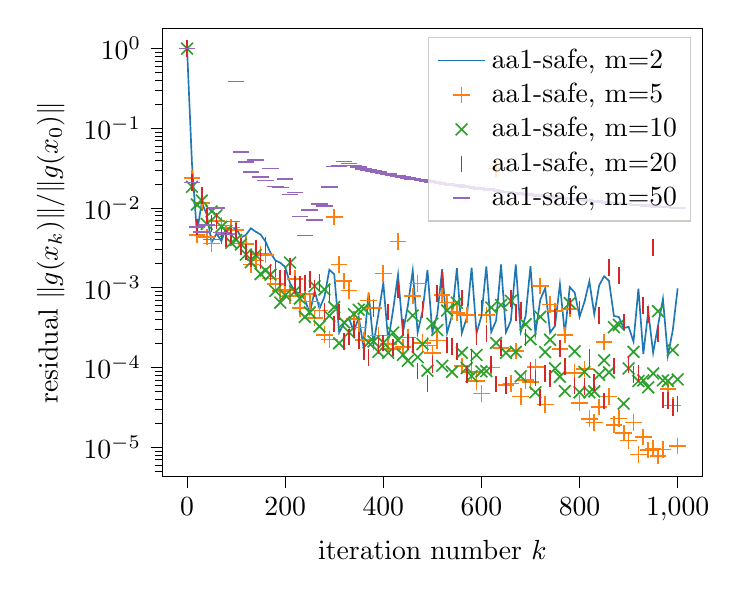
\begin{tikzpicture}

\definecolor{crimson2143940}{RGB}{214,39,40}
\definecolor{darkgray176}{RGB}{176,176,176}
\definecolor{darkorange25512714}{RGB}{255,127,14}
\definecolor{forestgreen4416044}{RGB}{44,160,44}
\definecolor{lightgray204}{RGB}{204,204,204}
\definecolor{mediumpurple148103189}{RGB}{148,103,189}
\definecolor{steelblue31119180}{RGB}{31,119,180}

\begin{axis}[
legend cell align={left},
legend style={fill opacity=0.8, draw opacity=1, text opacity=1, draw=lightgray204},
log basis y={10},
tick align=outside,
tick pos=left,
x grid style={darkgray176},
xlabel={iteration number \(\displaystyle k\)},
xmin=-50, xmax=1050,
xtick style={color=black},
y grid style={darkgray176},
ylabel={residual \(\displaystyle \norm{g(x_k)}/\norm{g(x_0)}\)},
ymin=4.27896517835089e-06, ymax=1.80156748743033,
ymode=log,
ytick style={color=black}
]
\addplot [semithick, steelblue31119180]
table {%
0 1
10 0.0359581514474822
20 0.00490599325465319
30 0.0117132837899294
40 0.0083498736036276
50 0.00370818777916238
60 0.00478731798166426
70 0.0038572532722462
80 0.00575903491221714
90 0.00520214098286327
100 0.00562623440702213
110 0.00428669115699809
120 0.00460288661823368
130 0.00557099029353831
140 0.00504456451363681
150 0.00464481631367055
160 0.00379192298723284
170 0.00273374953698956
180 0.00219965335632273
190 0.00205705396075004
200 0.00182564441461731
210 0.00113022197378547
220 0.000903707853232859
230 0.000843232077619485
240 0.000722003819230359
250 0.000475906965602033
260 0.000906277046897896
270 0.000548670341716041
280 0.000770209864021074
290 0.001678978154784
300 0.00147911952788934
310 0.000274591432668271
320 0.000358970720333932
330 0.000413044824696666
340 0.000283463626939296
350 0.000424309723138647
360 0.000176054944352072
370 0.000865566023415442
380 0.000193867648704285
390 0.000466872210538247
400 0.00114938833791134
410 0.000215695878037652
420 0.000529158541517708
430 0.00145767690674849
440 0.000274671757384632
450 0.000593314856836278
460 0.00164345099117982
470 0.000274295514010727
480 0.000512460565613341
490 0.0016717798392118
500 0.000275613096123428
510 0.000461533414208506
520 0.00171312026295822
530 0.000272039965580504
540 0.000448582517440047
550 0.00175877595790329
560 0.000270432806145712
570 0.000416372174959049
580 0.00178048608432772
590 0.000268909801704364
600 0.000439801846358164
610 0.00185583083580983
620 0.000278034005430263
630 0.000389031373256148
640 0.00196036927136551
650 0.000276775078254935
660 0.000385208466480644
670 0.0019546770850725
680 0.000278675972399789
690 0.000439292845636451
700 0.00186369682419338
710 0.000266990605870281
720 0.000707863875676191
730 0.000989605123365064
740 0.000273663907284589
750 0.000332629820231998
760 0.00110617890360696
770 0.000265673522389174
780 0.00102004312756697
790 0.000873978351064514
800 0.000430033817645183
810 0.000664680978952692
820 0.0012039795168909
830 0.000465190201265007
840 0.00106993084481944
850 0.00139336433294582
860 0.00122281038436545
870 0.00044311353575593
880 0.000430122254453925
890 0.000311453047107158
900 0.000323817365454646
910 0.000210770790494511
920 0.000975263102211454
930 0.000147546981240948
940 0.000505825941809792
950 0.000153032878453597
960 0.000335549169946042
970 0.000723658178237627
980 0.000139841394788654
990 0.00029160123676167
1000 0.000984069558484858
};
\addlegendentry{aa1-safe, m=2}
\addplot [semithick, darkorange25512714, mark=+, mark size=3, mark options={solid}, only marks]
table {%
0 1
10 0.02381412800765
20 0.00458182498049258
30 0.0116387067610535
40 0.00432250884445797
50 0.00357822493184303
60 0.00685634293058232
70 0.00602268984553705
80 0.0047080368062844
90 0.00570283806424191
100 0.00529100422689627
110 0.00357631898992692
120 0.00350887993208848
130 0.00194844932947285
140 0.00219612275545681
150 0.0026531162741625
160 0.00258986575963718
170 0.00130665531167392
180 0.00112189020232379
190 0.000906006076858634
200 0.000942134429124834
210 0.000793594262308771
220 0.00129782121085144
230 0.000552013270056156
240 0.000827096898441207
250 0.000670661683911561
260 0.000419205417951118
270 0.000517276244398655
280 0.000257740513720036
290 0.000224375299469405
300 0.0076854927841064
310 0.0019658322799978
320 0.00121320624745044
330 0.00092307690429109
340 0.000404548793578178
350 0.00031765191023225
360 0.000218943063200042
370 0.000693325468767236
380 0.000560245192283879
390 0.000251630607680585
400 0.00151563674530328
410 0.000198514685400347
420 0.000170705092261221
430 0.00379029552336146
440 0.000180356918793849
450 0.000237127273586266
460 0.000784930989112464
470 0.00112665668413204
480 0.000203857335730646
490 0.000189415892136266
500 0.000152588348143362
510 0.000217778312019713
520 0.000814777164964906
530 0.000651939477563168
540 0.000505042886297141
550 0.000484947801425454
560 0.000104650505009825
570 0.000455626848397152
580 8.84360195899475e-05
590 6.71887342068171e-05
600 4.72429403784976e-05
610 0.000454509880141022
620 9.96940583023863e-05
630 0.0311757256010751
640 0.000176623111192254
650 6.04659728531808e-05
660 6.26317061900009e-05
670 0.000161623531117076
680 4.34085638405131e-05
690 6.91199775529007e-05
700 6.56218252814593e-05
710 0.00010131616754621
720 0.00105684981141654
730 3.41549322512326e-05
740 0.000616820303193297
750 0.000511786992008098
760 0.000170211826195241
770 0.000254912116148822
780 0.000539178534274692
790 8.59557018526164e-05
800 3.59092575947768e-05
810 9.60919536431045e-05
820 2.27749720970121e-05
830 2.03021031325005e-05
840 3.18792555328433e-05
850 0.000207922348231583
860 4.3345131410386e-05
870 1.9096843253962e-05
880 2.28524384918277e-05
890 1.50642208094433e-05
900 1.21140021200067e-05
910 2.03991201027515e-05
920 8.06458544822047e-06
930 1.33955403413657e-05
940 9.25897240467389e-06
950 9.55245619165966e-06
960 7.70884454516347e-06
970 9.30955431129851e-06
980 5.35812857427164e-05
990 3.33375081354141e-05
1000 1.03405521835321e-05
};
\addlegendentry{aa1-safe, m=5}
\addplot [semithick, forestgreen4416044, mark=x, mark size=3, mark options={solid}, only marks]
table {%
0 1
10 0.0184843254586538
20 0.0110657272448688
30 0.0123967493035527
40 0.0063178287134402
50 0.0090781919825208
60 0.00811055551662201
70 0.00582768017849951
80 0.00516985154559303
90 0.00366101679425527
100 0.00397889584510863
110 0.00350426647534136
120 0.00261135520251543
130 0.00209205001555948
140 0.0025750154358244
150 0.00148751676563925
160 0.00164738052605089
170 0.00146001082920356
180 0.000911726922474212
190 0.00065206051032292
200 0.000804652090046185
210 0.00206746040900768
220 0.00090501523310856
230 0.000734436413950999
240 0.000430156667089059
250 0.000490620120104
260 0.00104677830077691
270 0.000327654361251825
280 0.000951850293680241
290 0.000445012583495314
300 0.000571562870875353
310 0.000201194055381753
320 0.000367086682560831
330 0.000276494824856059
340 0.000466041796116249
350 0.000529973575456384
360 0.000545568245547276
370 0.000205443618543322
380 0.000212256095324215
390 0.000157089673300989
400 0.000204783405620524
410 0.000153010655251834
420 0.000273895234659562
430 0.000220217263728768
440 0.000144076345032027
450 0.000121494101571603
460 0.000448326799163634
470 0.000134739950958091
480 0.000196462346972369
490 9.12018479468151e-05
500 0.000354707758424602
510 0.000295104267712408
520 0.000104622626954737
530 0.000519267982048681
540 8.79380538127282e-05
550 0.000649314616169495
560 0.000152756720084119
570 9.84547550878383e-05
580 7.77112030686538e-05
590 0.000143492144010356
600 8.90733866783624e-05
610 9.00124077747461e-05
620 0.000565016634285008
630 0.000202885282824509
640 0.00060776187786231
650 0.000152545738027734
660 0.000685220304879158
670 0.000156768938665596
680 7.74353899472402e-05
690 0.000347749549356765
700 0.000226941834097443
710 4.87179086479704e-05
720 0.000431963292450909
730 0.000156047379843263
740 0.000223023036106829
750 9.72561865490738e-05
760 7.64645719306412e-05
770 5.05628877061932e-05
780 0.000642225728717369
790 0.000159420337110223
800 4.86948513648037e-05
810 8.77745321219987e-05
820 4.87556339105873e-05
830 5.00988717236994e-05
840 8.09284348307277e-05
850 0.000122998586372067
860 8.67474224083446e-05
870 0.000320417543786133
880 0.000342250999044419
890 3.51054857271005e-05
900 9.72735718106241e-05
910 0.000156881760552028
920 6.75367587396123e-05
930 6.88995261477724e-05
940 5.63135066652707e-05
950 8.40819725627157e-05
960 0.000508442981755185
970 6.88604250953205e-05
980 6.76153339884989e-05
990 0.000165509288677631
1000 7.08982144777333e-05
};
\addlegendentry{aa1-safe, m=10}
\addplot [semithick, crimson2143940, mark=|, mark size=3, mark options={solid}, only marks]
table {%
0 1
10 0.0209862655282678
20 0.00579349022670721
30 0.0143778027843466
40 0.00790033828353336
50 0.00640725942706778
60 0.00684360949278387
70 0.00443775416289423
80 0.00413729666894626
90 0.00448072590158321
100 0.00503756531202672
110 0.00327538956989758
120 0.00279620617408425
130 0.00229682211136882
140 0.00313856898273622
150 0.00218663729609237
160 0.0033601152132383
170 0.00158087176688089
180 0.00173241547601165
190 0.00132527661148477
200 0.00132482326340311
210 0.00185892053287856
220 0.00109358190152827
230 0.00110017655597349
240 0.001144253122672
250 0.00127660346771303
260 0.000984983411302617
270 0.00117000774703428
280 0.000499900223853747
290 0.00084917297788378
300 0.000351566611215353
310 0.000498264571297366
320 0.000213325722074866
330 0.000239869840732358
340 0.000301301985540801
350 0.00021620347424037
360 0.000158481139637925
370 0.00013328843455534
380 0.000538813464115524
390 0.00018678602705301
400 0.000202256379991936
410 0.000495670050919322
420 0.000178665522937916
430 0.00095471484162724
440 0.000318295886120692
450 0.000208968192034427
460 0.000191492346758098
470 9.00131133015807e-05
480 0.000534832022829528
490 6.3055366803588e-05
500 0.000108358989293957
510 0.000849022415185787
520 0.00126852833495003
530 0.000192100313195498
540 0.000182952977747086
550 0.000157271468505953
560 0.000745048303321221
570 8.19140301621851e-05
580 0.000135573947947755
590 0.000244887784270894
600 0.000545999047713394
610 0.000266085637169837
620 0.000108045306800302
630 6.22884607915699e-05
640 0.000176253663577504
650 5.96415984085952e-05
660 0.000735946112788795
670 0.000488814336994577
680 0.000517555377345514
690 0.000237533646065367
700 9.17972922094044e-05
710 7.40403028412048e-05
720 4.17290303316366e-05
730 8.42734383810614e-05
740 7.26820391796839e-05
750 0.000429986627767521
760 0.000173982529076902
770 0.000102885381598512
780 0.000587884366371407
790 5.97634868478665e-05
800 0.000530037825630383
810 5.72889185693993e-05
820 0.000133947969382978
830 6.53148117548317e-05
840 0.000451539343453668
850 3.80103376382456e-05
860 0.00180967380893254
870 0.000103949253429405
880 0.00142837712520827
890 0.000370396773117852
900 0.000109014142053345
910 8.16039514955187e-05
920 8.45648661253665e-05
930 0.000600557247928766
940 0.000459499633466046
950 0.00321921344656015
960 0.000268815843158248
970 3.91717687623208e-05
980 3.8693334564779e-05
990 3.17232692316176e-05
1000 3.48631673664024e-05
};
\addlegendentry{aa1-safe, m=20}
\addplot [semithick, mediumpurple148103189, mark=-, mark size=3, mark options={solid}, only marks]
table {%
0 1
10 0.0208682251767126
20 0.00577503518826177
30 0.00495768008010777
40 0.00610544271990579
50 0.00402569257144147
60 0.010055381691613
70 0.00492734999486939
80 0.00466013014149801
90 0.0067960111603734
100 0.385931011462733
110 0.0507447956822265
120 0.0377318049335778
130 0.0281563258068044
140 0.040402987882438
150 0.0245954235632223
160 0.0221393696111954
170 0.0312268967664232
180 0.0186919131029477
190 0.0181340188795359
200 0.0232839291531027
210 0.0148277409462713
220 0.015668558227421
230 0.00783436065282466
240 0.0045051532965403
250 0.00952114902501186
260 0.00706466766663377
270 0.0111848252226229
280 0.0105231144154727
290 0.0182573745099442
300 0.0333078430764005
310 0.0336377110351895
320 0.0383732011752162
330 0.0361714778340724
340 0.0342483143060593
350 0.0326725432965453
360 0.0311179814784717
370 0.0300858081481709
380 0.028933382574306
390 0.0281350545651761
400 0.0270918459072631
410 0.0264892618732419
420 0.0255447431736026
430 0.0250823177147743
440 0.0242879295461952
450 0.0238836672234444
460 0.0232243732263147
470 0.0228449189810321
480 0.0222623068384578
490 0.0218663852471069
500 0.0213137049191946
510 0.0209525086371107
520 0.0203883545357399
530 0.0200833632823163
540 0.0195375807139386
550 0.0192793935833139
560 0.0187476320825809
570 0.0185322085918634
580 0.0180153481976915
590 0.0178311985943129
600 0.0173598908399596
610 0.0171810435082293
620 0.0167682954167402
630 0.0165654006614197
640 0.016162605978119
650 0.015993042606204
660 0.0156007941076546
670 0.0154560108091234
680 0.015074477610194
690 0.0150904345265875
700 0.0146614469112959
710 0.0146074423221688
720 0.0141967001947728
730 0.0141535224611346
740 0.0137809153560222
750 0.0137270691573508
760 0.0133688480226062
770 0.01332510990585
780 0.0129812882330387
790 0.0129463302780143
800 0.0126166584837644
810 0.0125893648141338
820 0.0122738778061964
830 0.0122530714875606
840 0.0119513841869469
850 0.011936462606206
860 0.0116481774751846
870 0.0116465669234652
880 0.0113635747072956
890 0.0113668822500835
900 0.0110957492427951
910 0.0111036555337334
920 0.0108420311512114
930 0.0108572105337769
940 0.010606139580556
950 0.0106241173801502
960 0.0103849920865356
970 0.0104053749558078
980 0.0101839915365615
990 0.0101998903778141
1000 0.00999073656149706
};
\addlegendentry{aa1-safe, m=50}
\end{axis}

\end{tikzpicture}

		}
		\caption{Residual norms for the elastic net regression problem.}
	\end{figure}
\end{frame}

\section{Summary}

\begin{frame}
	\frametitle{Summary}
\end{frame}

\section{Sources}

\begin{frame}[allowframebreaks]
	\frametitle{Sources}
	\nocite{*}
%	\bibliographystyle{plain}
%	\bibliography{bibliography}
	\printbibliography
\end{frame}


\begin{frame}[plain]
	\begin{center}
		\Large{{Thank you for your attention.}}
	\end{center}
\end{frame}

\frame[plain]

\end{document}
